
\documentclass[oneside,a4paper]{book}
%\pagestyle{headings}

\input{preamble}

% A B S T R A C T
% % % % % % % % % % % % % % % % % % % % % % % % % % % % % % % % % %
\chapter*{\centering Abstract}
\begin{tcolorbox}[colframe=black, colback=white, boxrule=1pt, arc=4mm]
\noindent
This thesis explores the reconstruction of online handwriting signals (e.g., pen trajectories) from offline images using transformer-based architectures. The study addresses the challenge of modeling handwriting kinematics, focusing on trajectories and velocity, through a transformer architecture.\par 
The BRUSH and UNIPEN datasets, representing diverse handwriting styles, 
were pre-processed to generate paired offline images and online signals.\par
The model leverages vision transformers for feature extraction and tests the incorporation of LSTMs to guide trajectory predictions.\par
Key contributions include a robust pre-processing pipeline with the inclusion of spatio-temporal signal alignment, 
a novel combination of transformers and LSTMs, and the introduction of metrics to evaluate both trajectory fidelity and shape consistency.\par
Results demonstrate the efficacy of the model in generating lifelike handwriting trajectories, 
achieving very good accuracy in coordinate prediction specifically for small signals, 
and high structural similarity between generated and target signals.\par
Future directions include extending this approach to historical documents by exploring knowledge transfer to other handwriting styles and fine-tuning capabilities, changing absolute coordinates to 
relative speed vectors, and refining datasets for broader utilization of data.
\end{tcolorbox}

% Supervisors
\vspace{1em}
\noindent
\textbf{Under the co-supervision of}\\
Prof. Rolf Ingold, Emeritus Professor, Department of Informatics, University of Fribourg\\
Dr. Andreas Fischer, Lecturer and Professor, Department of Informatics, University of Fribourg\\

\textit{With the assistance of Ray, Assistant \& PHD candidate, Faculty of Philosophy and History
Department, University of Basel}

% C O N T E N T S 
% % % % % % % % % % % % % % % % % % % % % % % % % % % % % % % % % % % % % % % %
\tableofcontents

%%%%%%%%%%%%%%%%%%%%%%%%%%%%%%%%%%
%%%% NEW CHAPTER %%%%%%%%%%%%%%%%%%%%%
%%%%%%%%%%%%%%%%%%%%%%%%%%%%%%%%%%
\chapter{Introduction}
\label{cha:introduction}

The invention of writing marks the start of History with its consistent written records and places handwriting at the root of human development. Many languages have birthed and died since then, and many alphabets and writing methods with them. Handwriting is rich in information, as every stroke will vary between languages, cultures, alphabets, and to an extent, individuals. Going even deeper, personal handwriting evolves and will be consistent but not identical throughout the life of a person. \\

Modern equipment allows the observation of many characteristics of handwriting. Numerical writings using connected pens and tablets can measure and record speed, elevation, and a plethora of other varied metrics during the transcription by an author. However, historical records do not have this luxury and analyzing such documents must be done from the limited analog support that is left (paper, papyrus, tablets...) and is constrained to an image of the handwritten text. \\

When analyzing an element of handwriting, two signals are distinguished: on one hand, the offline signal describes the fixed image of the handwriting and is typically the data available from historical documents. On the other hand, the online signal can be described as a suit of contiguous values obtained from the signal during its writing and is long-lost from historical documents. Such components can be very basic, such as the (x, y) coordinates of the pen, or more complex, such as the angle of the pen to the paper or its elevation at all times. \\

\begin{figure}[H]
    \centering
    \begin{minipage}[t]{0.45\textwidth}
        \centering
        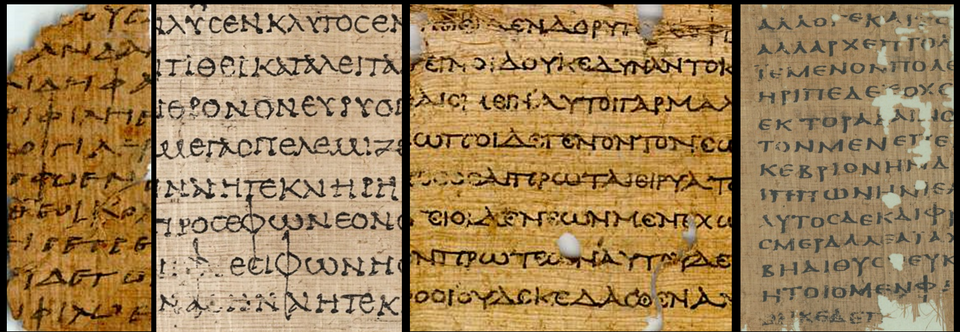
\includegraphics[width=\textwidth]{images/Intro/illiad.png}
        \caption{Iliad Papyrus from the EGRAPSA project collection}
        \label{fig:egrapsa_illiad}
    \end{minipage}
    \hfill
    \begin{minipage}[t]{0.45\textwidth}
        \centering
        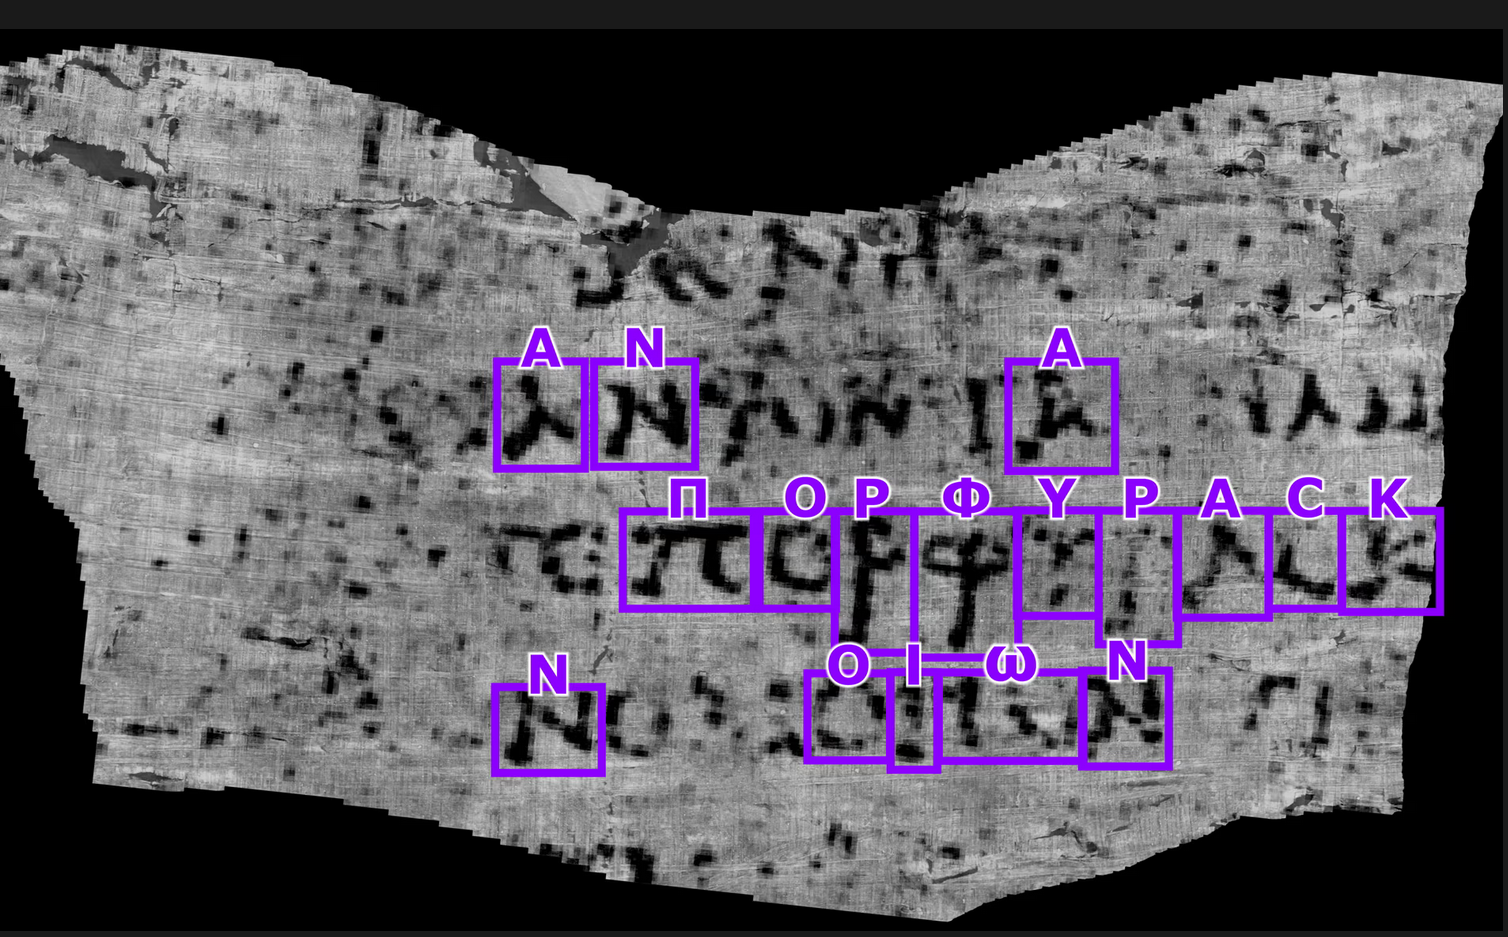
\includegraphics[width=\textwidth]{images/Intro/papyrus_vesuvius.png}
        \caption{Deciphered papyrus, Herculaneum collection, Vesuvius challenge}
        \label{fig:decyphered_vesuvius_papyrus}
    \end{minipage}
    \caption{Example of Papyrus as historical documents and the contribution from computer vision to the historical field}
    \label{fig:papyrus_examples}
\end{figure}

The present work is done as a collaboration with the university of Basel as part of the EGRAPSA project \cite{Egrapas}. The Department of Ancient Civilizations has a collection of original Greek papyrus, such as the Iliad (figure \ref{fig:egrapsa_illiad}), and coordinates its study. Computer vision has recently been the driving force of major breakthrough in the field of papyrus deciphering (Figure \ref{fig:decyphered_vesuvius_papyrus}), and we believe a study of the modeling of the handwriting of this collection can yield interesting archaeological value. For example, a good handwriting characterization could help in document dating, while individual handwriting descriptors could be used for authorship determination. Furthermore, such collections are finite and often limited whereas the recent computer vision models usually require large datasets for fine-tuning. The capacity to generate lifelike synthetic data could be very useful for that purpose.\\

Computer vision has been widely dominated by Convolutional Neural Networks (CNNs): deep learning models that use a set of predefined layers such as pooling or convolution used consecutively. They are tailored and have intrinsic bias toward two-dimensional visual data and prove themselves very good and efficient at extracting features from vision. However, the newest transformer-based architectures such as the encoder-decoders, used initially in large language models (LLMs), are becoming serious contenders in the computer vision field. Albeit very greedy for data compared to their historical counterpart due to their start from scratch, they are capable of extracting good features and work for a variety of classical vision problems. \\

This project aims to explore the capacity of a transformer-based architecture to produce a simple online signal of modern handwriting from its offline image. In order to prove this capacity, the concrete goal is to train a model to extract a vector of (x, y) coordinates using the image from a handwritten text. The resulting coordinate vector is assumed to be uniformly sampled as in the training data, introducing the notion of speed with each subsequent coordinate, making the model more than a simple skeletonization tool and forcing it to understand curvatures, accelerations, etc. to produce consistent trajectories. Furthermore, an additional goal is to know whether an analytical model's output could guide the transformer using a recurrent network in the loop as a proof of concept.

\chapter {Related Work}
Handwriting as a signal is hard to model. It is therefore difficult to reproduce or analyze an online data series from a two-dimensional image. Analytical models have proposed solutions to obtain mathematical descriptions of such signals, but this endeavor is very complex and requires a lot of computational efforts, which drives us to explore alternate solutions. \\

\begin{wrapfigure}{r}{6.0cm}
    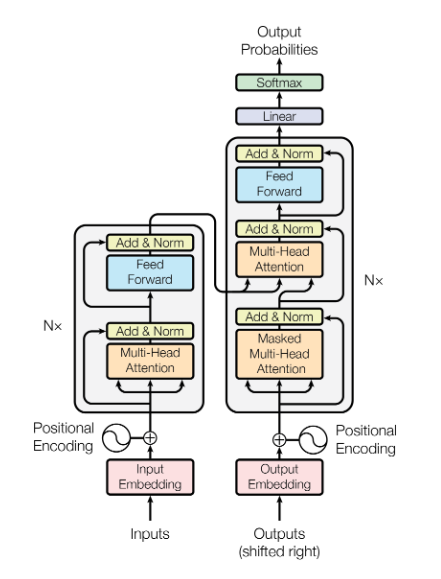
\includegraphics[width=6.0cm]{images/Related_works/attention_is_all.png}
    \label{fig:design_overview_attention_is_all}
    \caption{Design overview of the Transformer}
\end{wrapfigure}

Attention Is All You need \cite{DBLP:journals/corr/VaswaniSPUJGKP17} iterates over the work of Recurrent Neural Network (RNNs) based models for language-related tasks such as translation to introduce a staple of modern artificial intelligence: The transformer model. Whereas its predecessors were based on hidden states sequentially generated and passed along during training, the transformer proposes an innovative approach based entirely on \emph{Attention Mechanism} with parallelization at its core. This allowed the transformer to quickly out-perform its start-of-the-art counterparts and impose an efficient design that paved the ground for modern Large Language Models (LLMs). \\

The attention mechanism is the core operation of a transformer. The standard signal-processing models usually rely on Convolutional Neural Networks (CNNs), based on convolutions, to extract features from data. A CNN typically learns to adapt its convolutional kernel to analyze the data of a signal. Attention, on the other hand, focuses on the signal itself and the correlation between its elements. Attention Heads are based around scaled Dot-Product Attention. This operation has three inputs, A Query, A Key and a Value vector - or Q, K, V; with the Query and the Key sharing a dimension. The Query and Keys undergo a scaled multiplication; the result of which is passed through a softmax layer to obtain attention digits that are then transposed upon the Values vector. This computation is not often done on the whole signal at once: Rather, each element of the signal is subdivided into smaller sub-elements of equal dimensions that each undergo the attention mechanism. Each Attention processing unit is called a Head, and each Head attends to elements of dimensions \(D_{hidden}/N_{Heads}\).\par
Self-Attention refers to the utilization of an attention layer where Q, K and V are the same vector. Usually, self-attention is done on the signal itself. The outcome is an attention map that emphasizes the most important parts of the signal. \\

The Transformer model uses auto-regression to generate signals. The Inputs go through the encoder and a first token is fed through the decoder. Then, each generated token is added to the current output vector, shifted right, and fed again through the decoder until the end. For language-focused tasks, the fixed input can be a sentence to translate or a question to answer - The model then generates each word of the response until it is satisfied. The design overview of the figure \ref{fig:design_overview_attention_is_all} shows that the encoder passes the input through a self-attention layer meanwhile the decoder passes the target through a self-attention layer. These two Attention Maps are passed through a cross-Attention layer in the decoder, a feed-forward network, and a final softmax to obtain the next prediction. \par
In the decoder, the notion of masking (or causal masking) prevents each token to look into the future and only allows previous tokens to be attended to. The training data can be cut into independent subsignals where each "mini-output" is formed from the ground truth. The model is continuously asked to predict the next token from these mini-outputs as if it was generated by itself. This method is often referred to as teacher forcing and makes the model learn to predict on allegedly good tokens, helping convergence and making parallelization of the whole training possible. Not using the model's predictions during the training loop allows it to be free of the costly iterative constraint of autoregression.\par
For reference, the model described in Attention Is All You Need has 6 layers in the encoder and the decoder, a hidden dimension of 512, and 8 attention heads. \\

In 2021, the work of \emph{An image is Worth 16x16 Words} \cite{DBLP:journals/corr/abs-2010-11929} shows that although CNNs are still the de-facto state-of-the art for vision tasks, transformer-based architectures relying solely on Self-attention are able to achieve comparable performance. However, training with the same scale of datasets as CNNs results in poorer performance - an observation that can be reversed given enough data for the transformer. Their hypothesis is that the transformers lacks the inductive bias of the CNNs and therefore requires more examples for good generalization. To obtain good results on these tasks, ViT trained with 300M images. Further work on image transformers, such as studies on distillation (DeiT - \textit{Training data-efficient image transformers \& distillation through attention} \cite{DBLP:journals/corr/abs-2012-12877}), make the same observation and try to reduce the memory footprint and training dataset requirements of transformers through teacher-student distillation token intending to transmit a large ConvNet teacher's knowledge to a smaller transformer student. \\

\begin{figure}[H]
    \centering
    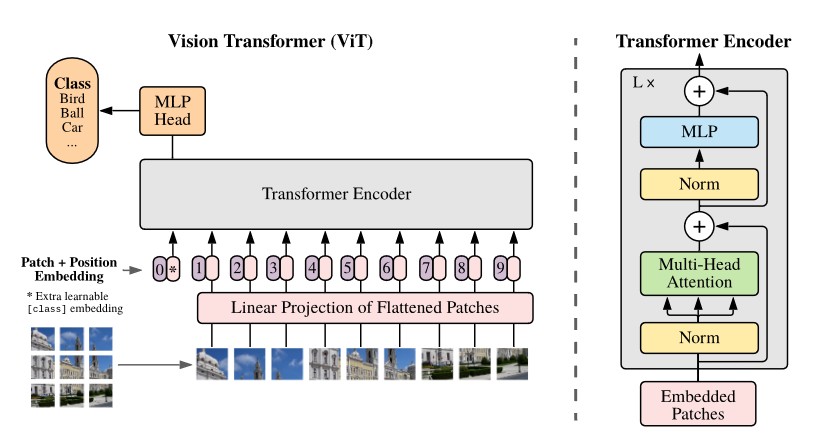
\includegraphics[scale=0.65]{images/Related_works/ViT.png}
    \caption{Design overview Vision Transformers (ViT)}
    \label{fig:vit_design}
\end{figure}

This transformer-based architecture, called Vision Transformer (ViT), addresses a significant challenge to achieve efficiency. By definition, the self-attention layer multiplies the signal by itself to compute its attention weights. However, quadratic complexity is infeasible when applied at the scale of images. Therefore, pixel-wise application of attention is not possible. \par
As shown in Figure \ref{fig:vit_design}, ViT makes images digestible for transformers by applying patchification followed by linear embedding. Assuming a square image of size \( n \times n \), a patch dimension of \( D_{\text{patches}} \), and a hidden dimension of \( Dim_{\text{hidden}} \) obtained by the linear embedding, the resulting complexity goes from quadratic with respect to the number of pixels — \( \mathcal{O}((n \times n)^2) \) — to quadratic with respect to the number of patches - \( \mathcal{O}((n_{\text{patch}} \times n_{\text{patch}})^2) = \mathcal{O}\left( \left( \frac{n}{D_{\text{patches}}} \times \frac{n}{D_{\text{patches}}} \right)^2 \right) \), as \( D_{hidden} \) is only relevant for the dot-product computation. In this context, the patch dimension \( D_{\text{patches}} \) must be large enough to reduce the number of tokens to acceptable dimensions for the self-attention, while still fitting within the hidden dimension \( D_{hidden} \) that will hold the information of a single patch.\\

\clearpage

\begin{wrapfigure}{r}{3.5cm}
    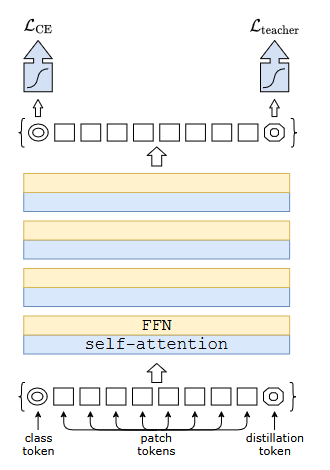
\includegraphics[width=3.5cm]{images/Related_works/deit_distill_token.png}
    \caption{Distillation token added to the DeiT model}
    \label{fig:deit_distill_token}
\end{wrapfigure}

Interestingly, ViT and DeiT share a similar architecture feature in the form of an additional token that holds different purposes.\par
For the former, the additional token is called a Classification token. The number of input tokens going into VIT's encoder is fixed and is equal to the number of patches in an image. With that in mind, there is no further reduction of dimensionality in the attention layers. However, the output of a classification task is usually obtained in the form of a last softmax layer with the dimension of the number of classes to predict. Rather than applying the softmax over the whole \(n_{patches}\) tokens, an additional token of \( D_{hidden} \) dimension is prepended to the sequence and is the input for the last prediction layer. This learnable token is attended to by all the other tokens (no causal mask) during the attention layers, and essentially becomes the output vector descriptor of the input image.\par
For the latter, the figure \ref{fig:deit_distill_token} shows that the distillation token is appended at the end of the input sequence in addition to a classification token that is also prepended at the start of said input. The last layer of DeiT Also ignores the 'working' tokens, focusing on the classification token and the distillation tokens to compute its losses. \\

One of the main work at the origin of this master project is the SET, SORT! doctoral thesis \cite{mohamedmoussa:tel-04583082}. SET, SORT ! and its associated paper \cite{10.1007/978-3-031-41676-7_5} presents a novel sub-stroke level Transformers for offline handwriting to online conversion. It shares a very similar purpose as the present project as it uses a transformer architecture to do offline-to-online signal conversion. The main difference is the format of the target online signal. \par
A handwriting signal such as a sentence or character is usually a composition of strokes, where a stroke is defined as a motion with the pen touching the paper at all times. In many handwriting databases, strokes are separated by a "Pen Up" signal indicating the start of a new stroke. Set, Sort! defines the level of sub-strokes, where a stroke can be further dissected amongst its conjunction points so that the signal is cut when it touches itself. Whereas a stroke can have ambiguous intersections where the line goes to many different directions, a substroke only ever goes from its start to its end point without loops. \par
The goal of their work is to transform a handwriting signal into a set of unique sub-strokes, and having the set ordered naturally. The results show that the simple act of correctly ordering a handwriting signal is already a challenge in itself - especially when considering not only the regular alphabet but additional symbols such as mathematical expressions - but also proves that transformers are able to perform such tasks. This ordering already requires the transformer to understand part of the ductus of the signal: it makes sense to look at speeds, trajectories, and relative positions to anticipate the next stroke, whether it is contiguous (end-to-start) or not (in case of PenUP, the next starting point can be anywhere). Our project differentiates itself by taking a deep dive into understanding the signal's shapes and speeds as our goal is to produce the generator coordinate vector of the offline image. \\

\clearpage

\begin{wrapfigure}{l}{6.8cm}
    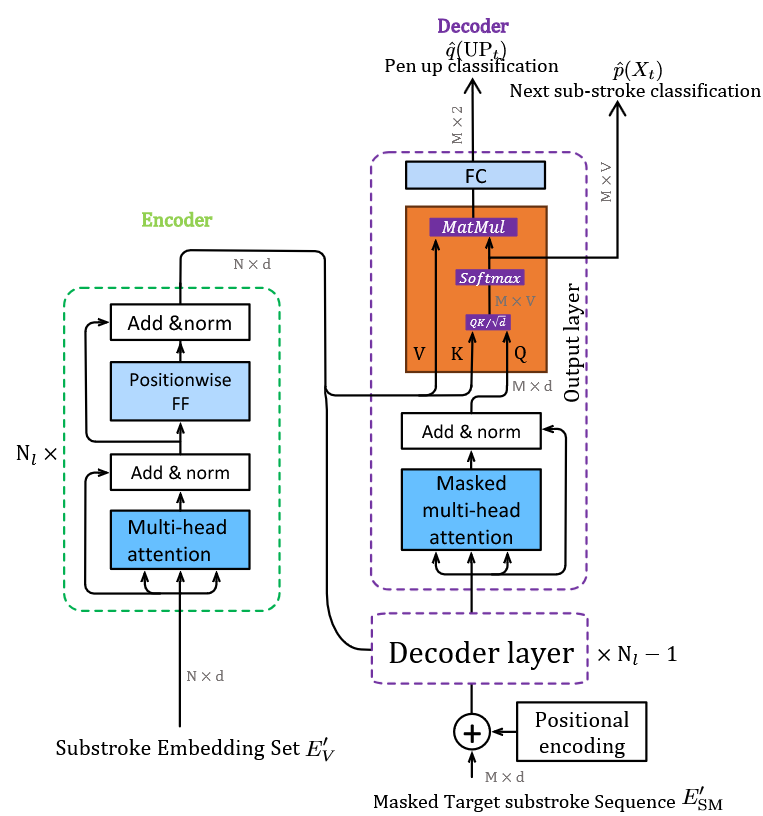
\includegraphics[width=6.8cm]{images/Related_works/set_sort architecture.png}
    \caption{Overview of the Set, Sort! architecture}
    \label{fig:set_sort_architecture}
\end{wrapfigure}

The architecture is based on a pair of transformers. The first one, SET, is very similar to a Vision transformer as it consists of an encoder taking coordinates as input and outputting descriptor vectors, acting as the eyes of the duo. The second, Sort, takes all the set's embeddings as well as the partial ordered set to generate the next index in the set, with the auto-regression continuing until the set is fully indexed. As shown in the figure \ref{fig:set_sort_architecture}, the Sort transformer is very traditional in its architecture, with the cross-attention being performed with the output of the target self-attention and the output of the decoder's embeddings. \\


Amongst RNNs, Long Short-Term Memory units (LSTMs) are a very popular choice for data series. Multiple work have studied the utilization of LSTMs with tangent objectives. \emph{Visual Representation of Online Handwriting Time Series for Deep Learning Parkinson’s Disease Detection} \cite{8893041} successfully uses a combination of Bidirectional LSTMs (BLSTM) and CNNs to ingest the online handwriting signal of patients to support diagnosis of Parkinson disease. \emph{Swin Transformer: Hierarchical Vision Transformer using Shifted Windows} \cite{liu2021swintransformerhierarchicalvision} proposes an iteration of the vision transformer using shifted windows as a general-purpose computer vision backend, and \emph{SwinLSTM: Improving Spatiotemporal Prediction Accuracy using Swin Transformer and LSTM} \cite{tang2023swinlstmimprovingspatiotemporalpredictionaccuracy} iterates over this design by adding LSTM units cells, transposing the prevalent design of CNNs and LSTMs combined to treat spatio-temporal data to a transformer-based environment. Our work intends to use a LSTM in the loop as a proof-of-concept "guiding unit" for the decoder, which could be transposed to other kind of units, such as more traditional analytical models.

\chapter {Proposed Solution}
This section lays out the proposed solution by offering an analysis of the training datasets and detailing the chosen architecture.

\section{Data}
Multiple datasets are available for use in handwriting research. As this project aims to investigate the capacities of a transformer model to extract a coordinate vector out of an offline image, the ideal dataset must contain recordings of the [x,y] coordinates for the pen. But what separates this model from a simple skeleton extractor tool, which are well studied and very accurate, is the additional focus put on the handwriting trajectories as well as speed: The resulting coordinate vector is interpreted as a single stroke of a pen, therefore, is must be ordered and within the same velocity.\par
The speed between two points could be added via a third dimension along the x,y coordinates. This would be equivalent to asking for the duration of the sub-stroke between points A and B, as the distance is contained within the two coordinates. To make this even simpler, the duration can be fixed to a constant number, making the third dimension obsolete as it is intrinsically contained in the signal itself. This means that shorter point-to-point pixel distances will result in slower strokes meanwhile high point-to-point pixel distances result in faster strokes. Regardless of the method used to convey speed (additional dimension for velocity, for time, or fixed sample rate), the training data must contain a notion of duration or speed: A signal can always be resampled as long as the initial sample rate is known or uniform between all data. \\

With these requirements in mind, four dataset names retained our attention: CHROME \cite{Mouchere2016CROHME}, A dataset from the eponymous competition available for mathematical handwritten expression recognition, containing a wide range of mathematical symbols; IAM \cite{791885}, an English handwriting database containing pages of scanned and labeled text from the university of Bern; UNIPEN \cite{IAM_UNIPEN_1999}, A large and public handwritten database made by a consortium of universities and entities across the world, and BRUSH \cite{kotani2020generating}, the Brown University Stylus handwriting dataset. \\

UNIPEN and Brush are perfect matches for this training as they both contain handwritten online signals in the form of coordinate signals with fixed sample rate (BRUSH, 10ms) or defined sample rate for each signal (UNIPEN).\par
Being made by a single entity, BRUSH has the advantage of uniformity which can reduce the risk for non-reducible errors due to difference of format or standardized material / acquisition process. On the other hand, this gives the advantage of diversity for UNIPEN, which includes more languages, more cultures, and therefore more ductus, meaning it could contain more overall information about generalized human handwriting. Ideally, as transformers are very data-hungry, the two datasets can be aligned on the same sample rate and mixed to form a large dataset and a sizable effort has been made at the start of the project to obtain aligned signals of both BRUSH and UNIPEN. Unfortunately, as the physical resources allotted to this master project are very limited with a single GPU machine, it is practically infeasible to train on a combined dataset as a single one is already out of acceptable training times. For this reason, Brush is the only dataset during experiments as its uniformity allows a simple random sampling from its data to produce consistent training signals for the model to learn meanwhile a random sampling of UNIPEN, which is bigger and more diverse, could produce inconsistent signals. In this case, bad results from the experiments would be very inconclusive as it would be very hard to identify the reason of the failure and discriminate between a design flaw or a bad dataset sampling preventing proper training. \\

\subsection{Datasets}
This section details the content of the two datasets used in the project, BRUSH and UNIPEN, as well as the processing that is done to obtain formatted training data. \par
In preamble, it is important to state that a transformer always expect the same number of input token in its encoder. For vision transformers, this translates as requiring a fixed image size. For this project, we have selected (96,96) pixels as our standard: The 96 value for the height is based on the average vertical length required by the datasets to represent a single line of handwriting and the shape is assigned by symmetry as square images are a simpler to manage compared to rectangular ones. \par
Both the BRUSH and UNIPEN datasets contain recordings of handwriting composed of the coordinates of the pen and the PenUp signal with a known sample rate. However, they do not contain the associated offline image that is one of the core of the training and objective of the transformer. As this project is a proof-of-concept of the transformer's capacities to learn such a concept, it is acceptable to work with "perfect images" generated by the coordinates. These perfect images reduce the chance of hardware or recording errors and the need for pre-processing as the lines are created at one pixel width. The conditions are simpler than that of real images as they do not contain any noise or perturbation, and thus the results of this report should be considered as experimental. Additional work  is required to translate these results to papyrus - for example, with the addition of pre-skeletonization of the images.

\begin{figure}[H]
    \centering
    
\includegraphics[scale=0.65]{images/Data/BRUSH/brush_example.png}
    \label{fig:brush_example}
    \caption{Example of two signals from the original BRUSH dataset. Left: Point-by-Point, Right: Line}
\end{figure}

The BRUSH dataset is composed of 170 writers providing around 160 drawings each. The drawings are all in English, and are a mix of cursive and manuscript characters with some additional symbols such as parenthesis, quotes or brackets. A drawing is represented as a coordinate signal of three dimensions with each element being (x, y, PenUp). Each writing represents a sentence and each datapoint is labeled by its character, which is not used yet but could prove very useful for further refinement of the training data. The figure \ref{fig:brush_example} shows two examples of BRUSH original sentences: The first row represents the drawing 5 of the writer 1 and the second row represents the drawing 5 of writer 5. The left section shows the coordinate vectors as points in a \(100 \times 700\) canvas (Height, Width). On the right side, an image is drawn by linking the coordinates with a one-pixel width line and lifting the pen when there is a PenUp signal.\\

\begin{table}[h]
    \centering
    \resizebox{\textwidth}{!}{%
    \begin{tabular}{lccp{2cm}p{2cm}p{2cm}p{2cm}p{2cm}}
    \toprule
        \textbf{Dataset} & \textbf{\# Signals} & \textbf{\# Datapoints} & \textbf{Avg. Image Shape} & \textbf{Max Image Shape} & \textbf{Avg. Signal Length} & \textbf{Signal Length Std} & \textbf{Min / Max Sig. Length} \\
    \midrule
        Original Brush         & 29,774   & 7.6M       & \(67 \times 408\) & \(184 \times 756\) & 257 & 98 & 2 / 1403 \\
        Strokes Brush          & 532,795  & 7.5M       & \(28 \times 22\)  & \(152 \times 368\) & 14  & 13 & 1 / 438  \\
        Limited Strokes Brush  & 537,431  & 7.5M       & \(28 \times 22\)  & \(96 \times 96\)   & 14  & 11 & 1 / 321  \\
    \bottomrule
    \end{tabular}%
    }
    \caption{BRUSH Dataset Statistics}
    \label{tab:brush_dataset_statistics}
\end{table}

The table \ref{tab:brush_dataset_statistics} lays out some statistical descriptions of the BRUSH dataset. The first row is the original data being read from the dataset - as in, complete sentences in handwriting. The second row represents the exact same data with each stroke being separated, meaning that each signal is cut along its "PenUp" instructions. Lastly, the third row represents the dataset with strokes limited to our maximum image shape, \(96 \times 96\). The exact cut process is explained in the next section. \\

The dataset originally contains around 30'000 sentences - or signals - spread amongst the 170 writers. This translates to ~500'000 strokes, as BRUSH is mainly composed of full sentences with multiple PenUp. It is interesting to remark that manuscript usually require more strokes than cursive and will therefore be cut in smaller atomic strokes. \par
The number of datapoints is also important as a signal is not equal to another in terms of information: A complete sentence contains more latent training data than a single character. BRUSH is composed of ~7.5M coordinates that the model can learn to predict. Logically, separating the strokes does not change that amount by a lot, although creating a new signal slightly decreases the number of datapoints that the model can predict as the first starting coordinate is always fed to the model.\par
Brush's average image shape is \(67 \times 408\) \((height \times width\)). This is clearly shown in the example signal with sentences being longer than they are tall. Extracting the strokes drastically reduces the average image shape to \(28 \times 22\), which is expected as many sub-character signals (the bar on the T, the dot in the i, etc) are essentially very small strokes.\par
The maximum image shape goes from \(184 \times 756\)  for the original signal to \(152 \times 368\)  when cut by strokes. For the limited strokes, the maximum shape is the one given by our requirement of \(96 \times 96\).\par
The original dataset has a mean signal length - as in, the amount of coordinates contained within a signal - of 257 with a std of 98. This is because the sentences contain a lot of characters, and thus, a lot of datapoints. When cut by strokes, this amount drastically decreases to an average of 14 datapoints per signal, with a std of 13. Again, this follows with many small strokes decreasing the general average. With a mean of 14 and a std of 13, the only affected images that are outside the scope with a shape above \(96 \times 96\) are outliers, and cutting them do not have a great impact on the mean length of signals.\par
Lastly, the signal length amplitude goes from [2;1403] for the original to [1; 438] for the strokes with the cuts on the PenUp and decreases again to [1;321] for the limited strokes.
 
\begin{figure}[H]
    \centering
    \begin{minipage}[t]{0.45\textwidth}
        \centering
        
\includegraphics[width=\textwidth]{images/Data/BRUSH/hist_brush_signals.png}
        \caption{Histograms of the original BRUSH dataset}
    \end{minipage}
    \hfill
    \begin{minipage}[t]{0.45\textwidth}
        \centering
        
\includegraphics[width=\textwidth]{images/Data/BRUSH/hist_brush_strokes.png}
        \caption{Histograms of the BRUSH dataset cut by strokes}
    \end{minipage}
    \caption{Histograms of the BRUSH dataset}
    \label{fig:brush_histograms}
\end{figure}

Looking at the histograms of the signal length before and after the stroke cut in the figure \ref{fig:brush_histograms} shows that the original signals are fairly evenly distributed around the mode at length ~300, meanwhile the strokes-separated dataset hit a very high spike and are densely compacted before length 50 with a significant drop in signal length.\\

Overall, the BRUSH dataset is very uniform. As it is captured by a single entity, it is easy to obtain a workable dataset of coordinate vectors with significant learning value.

\begin{figure}[H]
    \centering
    \begin{minipage}[t]{0.45\textwidth}
        \centering
        \includegraphics[width=\textwidth]{images/Data/Unipen/Unipen_ex1_diverse.png}
        \caption{Example of diverse data from UNIPEN}
        \label{fig:UNIPEN_diverse}
    \end{minipage}
    \hfill
    \begin{minipage}[t]{0.45\textwidth}
        \centering
        
\includegraphics[width=\textwidth]{images/Data/Unipen/overlapping.png}
        \caption{Example of overlapping signals}
        \label{fig:UNIPEN_overlapping}
    \end{minipage}
    \caption{Example of signals from the UNIPEN dataset}
    \label{fig:UNIPEN_examples}
\end{figure}

UNIPEN is a much larger dataset that is centered around entities each providing signals. In the following report, these entities will be called the UNIPEN providers. Signals are encoded in a text format defined by commands (X, Y, Penup, etc). Each entity has a configuration file (or configuration in the commands file) defining some characteristics of the recording, such as canvas size, sample rate, or quantization. \\

Having many providers is a double-edged sword: On one hand, this brings an amount of data that is non-negligible and a diversity in symbols and Ductus that is enormous. This is reflected on the figure \ref{fig:UNIPEN_diverse} that shows three samples from the same provider with respectively a list of symbols, digits, and letters. Usually, the configuration file contains the alphabet for the given signals, which could again be used to further refine the dataset. \par
On the other hand, having many providers means that the signals are non-homogeneous. This can bring difficulty in training as the Ductus might be incompatible. This also increases the amount of errors that are latent to having many experimental protocols for the recordings as well as many formats for the storage of the data. With our best efforts deployed on the parsing of the dataset, there still exist samples such as the figure \ref{fig:UNIPEN_overlapping} containing overlapping signals that were probably not recorded as is, with the leftmost image having a mix of a cursive 'a' and 'b'. Nevertheless, as this model focuses on strokes, this would not impact the final quality of data as each of these strokes would be separated. However, this indicates that further format-related problems can lie buried in the dataset. \par
In order to make UNIPEN's data compatible between providers and with BRUSH, an alignment of the coordinates is made on the time and spatial axis. Firstly, the sampling size (time domain) and the quantization (spatial domain) of the provider is retrieved in its config files. The sampling size is often given in points per second (PPS) or milliseconds, meanwhile the quantization represents the physical distance that a pixel represent, in pixel per inch (ppi) or pixel per millimeter (PPmm).\par
As we are operating on coordinates and not images, the change of quantization is straight forward: All quantization are converted to pixel per millimeter, and a ratio is computed between the provider's PPmm and the target PPmm. The full coordinate vector is then multiplied by this ratio to have the same physical measure for the same amount of pixels.\par
The re-sampling is computed by a simple interpolation of the data points between the current and target sampling rate via a function available under LGPL \cite{StackOverflowResampling}. For further security, the integrity of the signal could be checked after the re-sampling by verifying that the new sample rate does not violate the Nyquist–Shannon theorem and avoid distortions. In practicality, it can be assumed that the sampling rates are generally close enough to ignore this problem. The UNIPEN signals are aligned to 14PPmm and 100PPS as these values mix well with BRUSH and form our baseline.\\

\begin{table}[h]
    \centering
    \resizebox{\textwidth}{!}{%
    \begin{tabular}{lccp{2cm}p{2cm}p{2cm}p{2cm}p{2cm}}
    \toprule
        \textbf{Dataset} & \textbf{\# Signals} & \textbf{\# Datapoints} & \textbf{Avg. Image Shape} & \textbf{Max Image Shape} & \textbf{Avg. Signal Length} & \textbf{Signal Length Std} & \textbf{Min / Max Sig. Length} \\
    \midrule
        Original UNIPEN         & 314,428   & 69.9M       & \(146 \times 242\) & \(2482 \times 4431\) & 146 & 247 & 1 / 21,796 \\
        Strokes UNIPEN          & 770,039   & 69.4M       & \(85 \times 100\)  & \(2482 \times 3874\) & 85  & 159 & 1 / 21,796 \\
        Limited Strokes UNIPEN  & 2,514,172 & 69.4M       & \(49 \times 44\)   & \(96 \times 96\)     & 49  & 24  & 1 / 21,796 \\
    \bottomrule
    \end{tabular}%
    }
    \caption{UNIPEN Dataset Statistics}
    \label{tab:UNIPEN_dataset_statistics}
\end{table}

The table \ref{tab:UNIPEN_dataset_statistics} shows the statistics of the UNIPEN datasets. With all its providers combined, it is ten times larger than Brush, with 69.9M datapoints compared to the 7.6M of BRUSH. The UNIPEN images are in general much larger, with a maximum of \(2482 \times 4431\) pixels for the original images and \(2482 \times 3874\) pixels as strokes. This maximum image shape, along with the maximum signal length of \(21796\), hint at bad signals amongst the data as such lengths and shapes can hardly be attained in a single stroke. \par
The bigger average image shapes of \(146 \times 242\), or \(85 \times 100\) with strokes and \(49 \times 44\) for limited strokes can be a sign of longer and/or more rich data to train on. The general signal lengths are also much larger with an average of 49 datapoints per signal with limited strokes, although the massive outlier signals can be skewing the average up compared to healthy signals. \par

\begin{figure}[H]
    \centering
    \begin{minipage}[t]{0.45\textwidth}
        \centering
        \includegraphics[width=\textwidth]{images/Data/Unipen/Unipen_hist_original.png}
        \caption{Histograms of the original UNIPEN dataset}
    \end{minipage}
    \hfill
    \begin{minipage}[t]{0.45\textwidth}
        \centering
        \includegraphics[width=\textwidth]{images/Data/Unipen/Unipen_hist_original_strokes.png}
        \caption{Histograms of the UNIPEN dataset cut by strokes}
    \end{minipage}
    \caption{Histograms of the UNIPEN dataset}
    \label{fig:UNIPEN_histograms}
\end{figure}

The UNIPEN histograms in the figure \ref{fig:UNIPEN_histograms} paint a similar picture as the BRUSH histograms, with a large density of data in the low signal length and a lower trailing tail on the larger lengths. Most of the data are contained within the 0-200 range, with a mode slightly before 100. \\

As a conclusion, BRUSH is much easier to work with as a homogeneous dataset with a limited amount of signals (7M data points) but a rather good consistency and quality. It only allows training on the English language, more specifically cursive and manuscript with a few symbols, which would produce specialized models but give them a good chance to learn this ductus. On the other hands, UNIPEN is richer and more diverse as a non-homogeneous dataset in terms of alphabet and Ductus, but has more challenges related to formatting and the source of data being spread amongst many entities. \par
Ideally, both datasets could be used, bringing the total number of signals available for this project within the bounds of acceptable for the training of a transformer model - we would have a total of 80M datapoints, where ViT uses 300M images for image classification. \\

\subsection{Data Processing}
This section describes step-by-step the pre-processing pipeline executed on the dataset to go from raw data to coordinate data to training-ready data.

\begin{figure}[H]
    \centering
    
\includegraphics[scale=0.5]{images/Data/PreProcess/preprocess_pipeline.png}
    \caption{Overview of the Pre-processing Pipeline}
    \label{fig:preprocess_pipeline}
\end{figure}

The overview of the pre-processing pipeline in the figure \ref{fig:preprocess_pipeline} shows two out of the three major transformation applied to the raw signals.\par
Firstly, the leftmost part shows the two data sources being read - BRUSH and UNIPEN, each with its native formats. As explained in the previous section, the data sources are responsible for aligning the signals in a standardized format of vector coordinates of (x, y) with a constant sampling rate and pixel quantization in order to allow the model to have a point of reference to infer speeds and trajectories. \par
Secondly, the rightmost part shows the common pre-processing applied to all the data sources. The coordinate vectors obtained from reading the raw data sources are not yet usable as they are abstract handwriting signals with a content tailored by their separate recording protocols - for example, BRUSH signals will contain a full sentence per image whereas the UNIPEN data vary from provider to provider, and can contain from one character to an entire multi-lines page of text. \par
Thirdly, these signals are separated into atomic training signals in order to obtain a parallelized training dataset.\\

The Pre-Processing aims to obtain a single stroke per signal and has to limit the images to a shape of \(96\times96\) pixels. Additionally, it tries to correct recording / format / parsing errors to obtain healthier data, as such errors will induce irreducible errors for the model and risk disrupting its training. Ultimately, this pipeline runs in seven sequential steps.\par
The following section follows the steps of a signal from BRUSH being pre-processed.

\begin{enumerate}
  \item[0.] Original Signal
\end{enumerate}

\begin{figure}[H]
    \centering
    
\includegraphics[scale=0.3]{images/Data/PreProcess/1_original_signal.png}
    \caption{BRUSH signal at step 0: Original signal}
    \label{fig:0_original}
\end{figure}

The signal shown in the figure \ref{fig:0_original} is an out-of-the-box BRUSH signal and is typically a full sentence written in cursive. It is composed of two words - Qualms Politics - followed by some symbol - ; ] - and an A. \\

\begin{enumerate}
  \item[1.] Stroke Separation
\end{enumerate}
The signal is separated along its PenUp instructions.

\begin{figure}[H]
    \centering
    
\includegraphics[scale=0.3]{images/Data/PreProcess/2_signal_strokes.png}
    \caption{BRUSH signal after step 1: Strokes Separation}
    \label{fig:1_strokes}
\end{figure}

In the figure \ref{fig:1_strokes}, the signal has been cut into 10 separate strokes. Each signal in these images can be written without getting the PenUp once, meaning the model will be able to predict it from start to end. Each signal is iteratively added to a growing black part - this is because the coordinates are absolute and each signal is represented at its location in the original image. Some signals - such as the single points on the 'i', become insignificant and hold very little information for the training once separated from their context.

\begin{enumerate}
  \item[2.] False Start Removal
\end{enumerate}
Some signals take some time to start with the starting coordinate or (0,0) being repeated for a large amount of time at the beginning of the coordinate vector. The most probable cause is an early start to their recording with the first few instants capturing an immobile pen. This has two major impacts on the data health: it creates artificially longer signals that do not contain information; and worse, it can teach the model to wait for a period of time before starting a signal. The False start removal step analyzes the start of the signal and removes eventual copies of the starting coordinate. This step is inherently not visual.

\begin{enumerate}
  \item[3.] Windows Cut
\end{enumerate}
This step has been deprecated and was an initial way to cut the signals every \textit{|window|} datapoint to reduce image sizes. However, the amount of data points is a rather bad predictor of image length and has been deprecated in favor of step 5 - outlier cut. \\

\begin{enumerate}
  \item[4.] Re-alignement
\end{enumerate}

The signals are re-aligned to the origin \([0,0]\) position. 

\begin{figure}[H]
    \centering
    
\includegraphics[scale=0.3]{images/Data/PreProcess/3_signals_aligned.png}
    \caption{BRUSH signal after step 4: Aligned signals}
    \label{fig:2_alignement}
\end{figure}

Each \([x_i, y_i]\) coordinate in the signals in the figure \ref{fig:2_alignement} goes through the following transformation:
\[ x_i' = x_i - (\min(x) - P) \]
\[ y_i' = y_i - (\min(y) - P) \]
This aligns every signal to the image origins at \([0, 0]\) given a safety padding value \(P\) of three pixels. Similarly, the creation of images automatically adjusts the canvas size to fit the exact signal, meaning the right and bottom parts of the images always fit the signal's bounding boxes except for a similar padding of three pixels. \\

\begin{enumerate}
  \item[5.] Suspicious Pen-Up removal
\end{enumerate}

In an effort to reduce the amount of erroneous signals in UNIPEN, an investigation into the suspiciously long signals has revealed that some datapoints are separated by a very long distance and are typically line returns on the physical support of the handwriting. This is very indicative of a missing PenUp command that should be separating these strokes. In order to resolve the issue, signals are scanned and the distance between each data point is computed. As the signal represent the kinematic of a pen in a real hand and because teleportation and time travel are unfortunately under-studied and very rarely observed, it is impossible for the pen to travel such high distances in the given time between points. The distance between two samples can be seen as bounded by a distance. From that bounding circle, we define a threshold of acceptable distance and artificially separate the signal in two as if a PenUp command was present upon detection. \\

\begin{enumerate}
  \item[6.] Outliers removal
\end{enumerate}

All images generated by the signals must fit within the maximum image size of the transformer's input. This step is responsible for downsizing every image with a shape above the selected one.\par
It is called Outliers Removal as an initial implementation of this step was to compute the mean and standard deviation of the image shapes and resize every image above \(mean + 2 \times std\) to the mean. This method has been deprecated as explained in section \ref{rejected_features}.\par
The outlier removal step is implemented in a much simpler process: Every signal generating an image with a shape above the threshold is cut in two at its middle point until the generated image shapes all fit the given threshold. \\

\begin{figure}[H]
    \centering
    
\includegraphics[scale=0.3]{images/Data/PreProcess/4_outliers_removed.png}
    \caption{BRUSH signal after step 6: Outlier removal}
    \label{fig:3_outlier_removal}
\end{figure}

The ten images of the BRUSH signal are spread into 14 sub-signals displayed in the figure \ref{fig:3_outlier_removal}. The two cursive strokes "Qualms" and "Politics" were generating images above the threshold and have been cut each into three sub-signals fitting the transformer bounds.\par
It is evident that the generated sub-signals are less than perfect: On one hand, the signals after the first lack the inertia of the previous sub-signals and are thus adding an irreducible noise to the data as the model cannot guess that the signal does not truly start there; on the other hand, some of the sub-signals being generated can be illegible as cutting a character into multiple parts might never be done by a regular handwriting, which is often the case for cursive. A promising axis of enhancement of the dataset is by generating better sub-signals - for example, by identifying potential cut points that have low impact on the signal integrity. For BRUSH, this can be done via using the point-to-character labialization built within the raw data. For UNIPEN or other datasets, this will likely require analyze and heuristics.\\

\begin{enumerate}
  \item[7.] Re-alignement
\end{enumerate}
Lastly, the signal is re-aligned in order to get rid of the offsets caused by the previous outlier cuts. \par

\begin{figure}[H]
    \centering
    
\includegraphics[scale=0.3]{images/Data/PreProcess/5_signals_aligned.png}
    \caption{BRUSH signal after step 7: Final Signal Alignment}
    \label{fig:4_alignement}
\end{figure}

The 14 re-aligned sub-signals in the figure \ref{fig:4_alignement} are the final data generated from the original Qualms Politics ;[A sentence, composed of individual strokes generating images of maximum \(96 \times 96\) pixels aligned to the origin.\\

The final sub-signals are almost ready for the model. To make the training parallelizable, they undergo a final transformation into atomic training items.

\begin{figure}[H]
    \centering
    
\includegraphics[scale=0.7]{images/Data/PreProcess/diagrams-batchification.drawio.png}
    \caption{Overview of the process from vectors to parallelized sub-signals}
    \label{fig:batchification}
\end{figure}

Considering each signal as a 'sequence' of \(n\) coordinates in Grey in the figure \ref{fig:batchification}, the same amount of training sub-sequences can be extracted by generating an independent training sample per predictable datapoint. A training sub-sequence is defined as a sequence of coordinates in red with a predictable coordinate, the label, in blue.\par 
By design, the model's goal is not to determine the start of sequences and the starting coordinate is never predicted. Thus, a training sub-sequence always has at least one coordinate. However, an End Of Sequence (EOS) token is added to each sequence in order to give the capacity and teach the model to stop generating signals when no further pixels are to be drawn. This EOS has to be unattainable by a signal in order to remain unambiguous, but close enough to valid data as the model could likely learn a validity domain from the datasets. As such, the \([-1;-1]\) coordinates are selected as negative coordinates are never valid considering an image shape.\par
The image computed on the whole complete signal is assigned to each sub-signal as the model has access to the whole offline data at every point during the inference. Finally, each image, sequence and subsequence is saved to disk. This has two upsides: it allows the transfer of datasets between systems for reproducibility purposes and removes any constraint on memory as the datasets are very large. This remains a trade-off as the data has to be read from files during each batch which is a costly operation. To reduce this impact, each sequence is saved to individual files in order to be quickly retrievable on demand via its unique ID.

\subsection{Data Augmentation}
The model always works with the partial subsequences during training in the prediction of the next coordinate. As the images are generated from said coordinates, they form a perfect match that the model can rely on. But during inference with auto-regression, the coordinates generated by the model can diverge from the image's skeleton and the model can quickly lose track of the trajectory being made. This typically ends up with the generated signal looping over itself, keeping a consistent trajectory and speed, but being completely dissociated from the offline image and unable to correct itself. Preventing the model to always expect the coordinates to line up with the skeleton can improve its auto-regression efficiency and help it generalize its understanding of the coordinate-to-image relationship, making it more robust to noise in the process.

\begin{figure}[H]
    \centering
    \begin{minipage}[t]{0.45\textwidth}
        \centering
        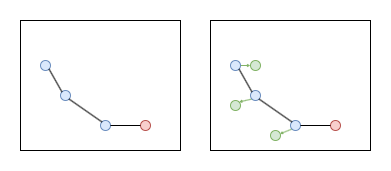
\includegraphics[width=\textwidth]{images/Experiments/Augmentations/diagram_Gaussian_noise.png}
        \caption{Sketch representation of adding Gaussian noise to coordinates}
        \label{fig:Gaussian_noise_to_coordinates}
    \end{minipage}%
    \hfill
    \begin{minipage}[t]{0.45\textwidth}
        \centering
        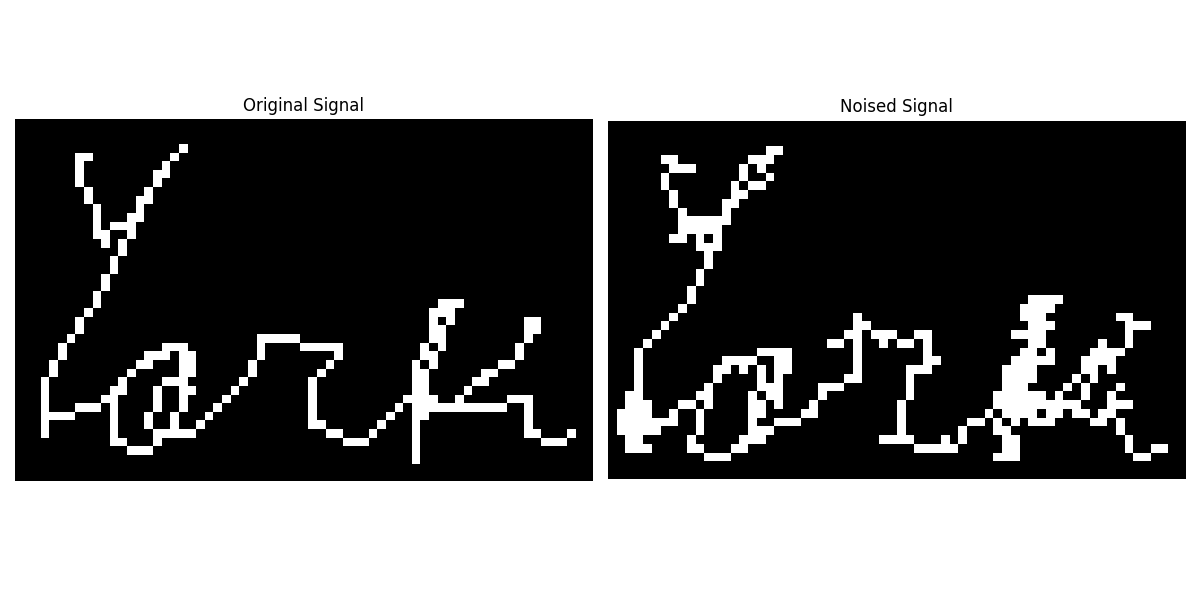
\includegraphics[width=\textwidth]{images/Experiments/Augmentations/Gaussian_noise_ex_2.png}
        \caption{Example of a signal pre- and post-augmentation}
        \label{fig:gaussian_noise_pre_post}
    \end{minipage}
    \caption{Addition of Gaussian Noise to the coordinate vectors}
    \label{fig:Gaussian_noise_explaination}
\end{figure}

Adding a Gaussian noise to the coordinates makes every data point close to but not exactly on the skeleton as represented in the figure \ref{fig:Gaussian_noise_to_coordinates}. This intends to force the model to account for inaccuracies of measurements and general noise in the data. In the figure \ref{fig:gaussian_noise_pre_post}, the left image represents the original image generated by the signal that is being sent to the vision encoder of the transformer, while the right part shows a representation of the noised coordinates that are sent to the decoder as the sequence of previous coordinates. The Gaussian noise is fixed to a mean of 0 and an STD of 1, making the points' offsets centered on the original point while being displaced a few pixels in each direction to keep the signal somehow consistent with the image. The coordinates to predict are never noised: making the model predict a point disjointed from the skeleton would be counter-productive.

\section{Design overview}
This section details the design of the proposed solution by reviewing the architecture of the model, discussing multiple details such as the LSTM utilization, padding, layer normalization and causal mask, the losses and metrics used for training and evaluating models, and finishes by detailing some features that did not make the final cut as they were judged non-beneficial in the long term.

\subsection{Architecture}
The architecture draws significant inspiration from three foundational works on transformers detailed in Chapter 2: Related Works — Attention Is All You Need, Vision Transformers, and SET, SORT!. These influential studies provide the groundwork for our design choices, and their ideas are reflected throughout the final architecture.

\begin{figure}[H]
    \centering
    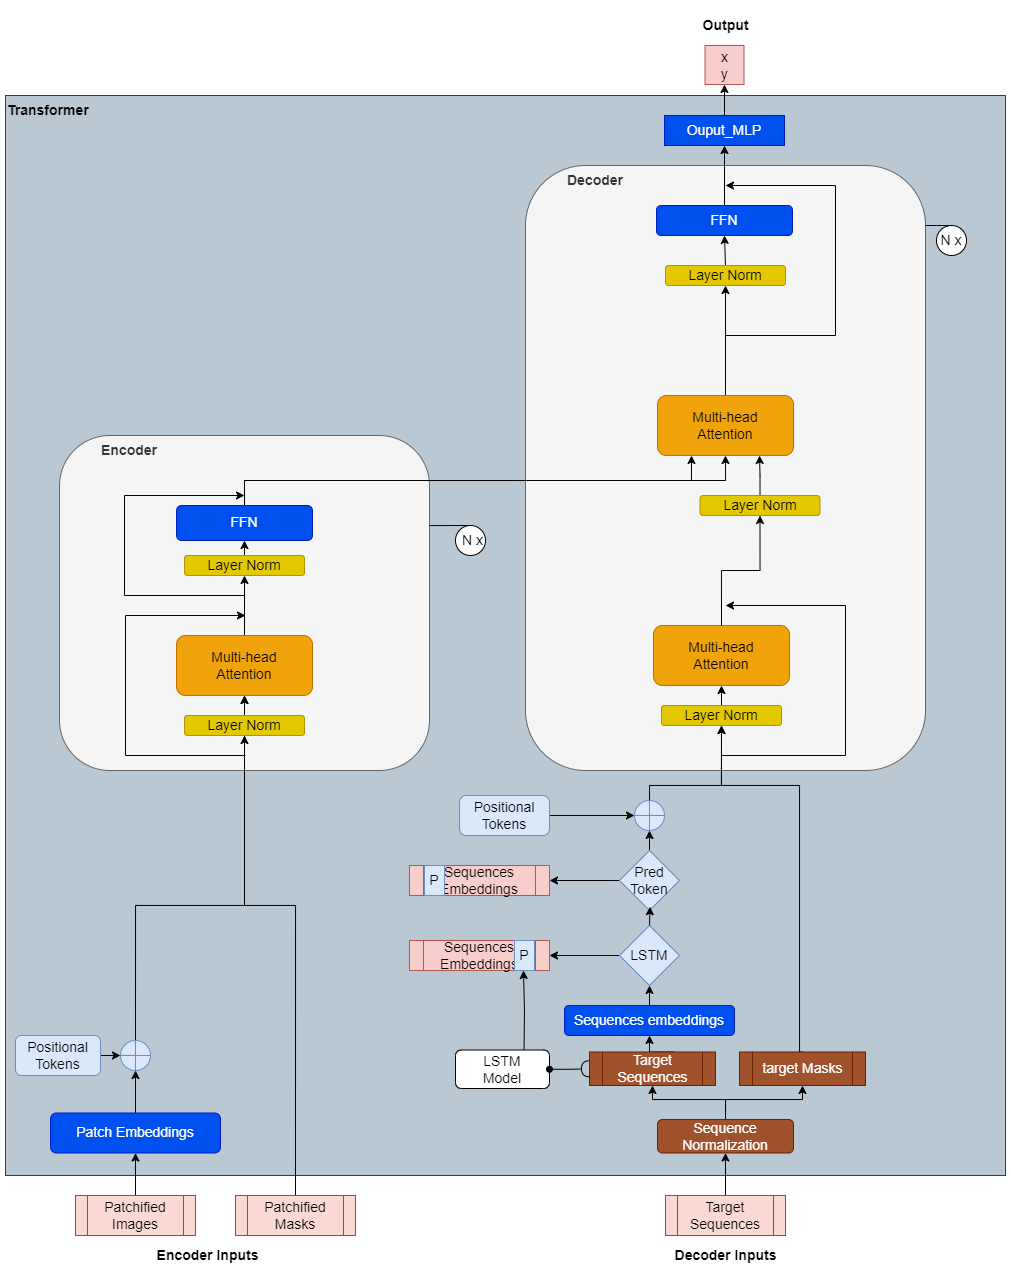
\includegraphics[scale=0.4]{images/Design/architecture.png}
    \caption{Architecture Overview of the proposed model}
    \label{fig:architecture_overview}
\end{figure}

The Final architecture is entirely laid out in the figure \ref{fig:architecture_overview}. The model is a transformer composed of two parts: A vision encoder based on the ViT architecture and a decoder mixing the target sequences with the output of the vision encoder. In total, it has three inputs and one output.\\

The first pair of inputs goes into the vision encoder: It is the offline image that the model looks to predict the coordinates. Specifically, we follow ViT's architecture: The images are cut into patches, with the vector of patches called the "Patchified images". The patchification process creates a Padding mask that is also ingested by the encoder as explained in the next section. The flattened patches go through a linear embedding layer to obtain a patch embedding for each patch of dimension \(D_{hidden}\). In order to avoid a reduction of dimensionality, we fix the image size at \(96 \times 96\) with a patch size of \(16 \times 16\) and a hidden dimension of \(256\). This means the patchified images are split into \(Size_{image}/Size_{patch} = 96/16 = 6\) patches along each dimension for a total of \(6 \times 6 = 36\) patches. Each patch contains \(16 \times 16 = 256\) pixels and is projected onto a vector of size 256, facilitating the work of the initial embedding layer.\par
A positional token is added to each patch embedding. The positional token is a standard Cosine/Sine-based positional generator function.\par
These embeddings and masks are passed through a Multi-Head self-attention (MHSA) with a pre-layer normalization. The MHSA in the encoder is tasked with finding the important part of the images to look through - intuitively, the encoder should find and focus on the handwriting signal contained within the image. The accompanying patchified masks is used to reduce useless computation in the first MHSA by setting the attention of padded masks to \(-\inf\).\par
The output of the first MHSA with the addition of a residual connection from the input is passed to a Feed-Forward Network (FFN). The FFN is composed of three parts - A fully connected linear layer that dilates the signal to \(n \times D_{hidden}\), an activation function, and a second fully connected linear layer that shrinks the dimension back to \(D_{hidden}\). The expansion ratio and the activation are typically hyperparameters of the transformer.\par
The result of this FFN with the addition of a residual connection from the previous layer goes directly to the decoder for further processing. The encoder layer is repeated \(n\) times.\\

The third input is the target sequences going into the decoder. The target sequence is a sequence of coordinates of unbounded length that represents the current sequence of coordinates form which the next coordinate is predicted.\par
Similarly to the encoder's images that are bounded to shapes of \(96 \times 96\) pixels as the MHSA expects fixed-size inputs, the decoder has an expectation of size for the target sequences. However, there is no intrinsic limit to the length of a handwriting signal, although an average length of strokes can be computed form the datasets and can generally be expected. Whereas the encoder's limitation limits the size of input images, the decoder's limitation is on the number of coordinates that the model is able to see before predicting the next. This is very close to the notion of context length or horizon in LLMs where this limitation impacts the length of the sentence that the model can 'store' and look through when thinking about the next word. The model has an auto regression sequence length of \(100\) coordinates as a trade-off between having more context that could be used for better prediction at the cost of memory and computational complexity wasted on token that may rarely be used. Every sequence that is smaller than this sequence length is padded with a similar notion of masking meanwhile every sequence that is larger than this sequence length is clipped to the sequence length. The fist (leftmost) tokens are discarded to always keep the more current coordinates.\par
Each input coordinate is passed through a similar linear layer as the encoder to obtain Sequence embeddings of the same size \(D_{hidden}\). This means each two-dimensional coordinate is projected into a 256-wide embedding. This is essential: the tokens dimensions must be aligned between the encoder and the decoder for the second cross multi-head attention. Furthermore, projecting the coordinates into higher dimensions has no risk of loss of information compared to reduced dimensionality. \par
Taking inspiration from ViT's classification tokens and DeiT's distillation tokens, we propose two additional tokens for the model. The first one allows an LSTM to guide the generation of the next prediction token by proposing the next most likely coordinates based on the current sequence of coordinates. Although the LSTM has no access to the image and thus cannot be expected to correctly predict a full handwriting online signal based on an image, it could help to generate better trajectories and avoid unlikely changes of direction as further explained in the section \ref{Usage_of_lstm}. Secondly, A Prediction token can be prepended to the sequence. The prediction token is identical in usage to the classification token: A learnable token of dimension \(D_{hidden}\) is prepended to the sequence and will be present at every step of the subsequent MHA layers. The final MLP layer usually uses the full sequence of output to generate the next prediction token. When prediction token is present, it only uses it to compute the \([x, y]\) coordinates.\par
As in the encoder, the sequence embeddings are added to positional tokens. Positional tokens are generated from the same Sine-Cosine based function. Positional tokens are used to uniquely identify each token in the sequence in the MHA layers. In both cases, the positional tokens can either stay at their fixed value or can be made learnable, in which case the model is allowed to find better positional tokens. The initial value of the tokens is always the sine-cosine function.\par
The attention output of this sequence MHSA is mixed with the output of the encoder in the second multi-head attention layer of the decoder. This is where offline and online signals are mixed, with the query and key being the vision output and the values being the sequences output.\par
The result of the cross-attention is passed through a FFN layer. The transformer has a last MLP layer that computes the predicted coordinates, going from token(s) of dimension \(D_{hidden}\) to 2. This last MLP's input is either the Prediction token alone or the full sequence of attention tokens previously generated.\\

From this architecture, we define three 'structural' (hyper-)parameters in light blue that fundamentally impact the flow of the transformer: The Positional tokens being learnable, the presence-absence of an LSTM unit, and the utilization of the Prediction Token. We define them as structural as a distinction from standard hyperparameters that usually refer to parameters which value can be slightly tuned such as learning rate, number of layers, or activation functions.

\subsection{Utilization of LSTMs} \label{Usage_of_lstm}
As discussed in the related works, LSTMs are RNNs that are very efficient when working on data series information and they have been tested and are successful when working with online handwriting signals. At first glance, as offline images are not sequential data, the LSTMs appear unadapted to the task. However, the transformer's goal is to predict a consistent coordinate vector with respect to general expected handwriting trajectories and speed. For such task, a lightweight LSTM model may be able to help guide the decoder.

\begin{figure}[H]
    \centering
    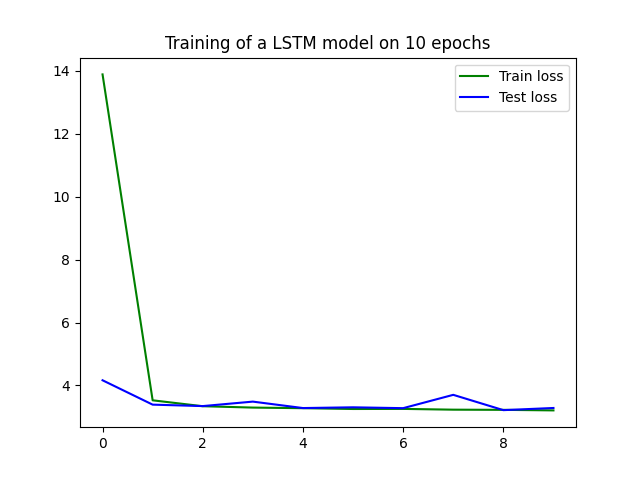
\includegraphics[scale=0.3]{images/Design/lstm_train_test_losses.png}
\caption{Training of a LSTM model on 10 epochs}
\label{fig:lstm_training}
\end{figure}

The formatted data extracted for the transformer's training task is perfectly adapted to the LSTM training as it contains sub-sequences of signal of length \(j\) with the label being the next token to predict at index \(j+1\). With the same datasets, we train an LSTM model to predict tokens based on previous sequences of coordinates. The figure \ref{fig:lstm_training} shows the training of a bidirectional LSTM model on ten epochs. The training appears to have a very fast convergence rate, and is hitting a loss plateau of ~3 pixels. The loss value is the average Euclidean distance between the predicted and expected signals, meaning the LSTM model is able to consistently predict the next coordinate with less than 3 pixels of its target based on the current trajectory alone. As the model has no access to the handwriting offline image, it cannot perfectly predict next coordinates and is rather tasked with generating a 'likely' coordinate taking into account inertia, curves, etc. \par
We fix the hidden size of the LSTM at the same \(D_{hidden}\) of the transformer. During pre-training, an MLP layer predicts two-dimensional \([x,y]\) coordinates from the last hidden state of the LSTM. For the integration into the transformer, the MLP layer is discarded and the last hidden state of the LSTM layer has the perfect dimensionality to be added as a token of the sequence. The LSTM is pre-trained with this protocol and its weights are frozen when being incorporated as a module of the transformer for training and inference.\par
The LSTM model trains on the unaugmented dataset: The goal of the Gaussian Noise augmentation is to prevent the transformer model that has access to the offline image to expect a perfect match of the target sequences coordinates on the skeleton. As the LSTM has no access to the image, there is no point in adding an artificial noise to the coordinates. \\

\subsection{Image Padding and Masking}

All images generated by the signals are cut at a shape of maximum \(96 \times 96\) pixels. From the dataset statistics, BRUSH and UNIPEN have an average image shape of respectively \(29 \times 22\) and \(49 \times 44\) pixels. This means that in most cases, images will be smaller than the expected shape. In such cases, the image has to be extended in order to fit the exact expected image shape and produce the right number of patches for the encoder.\par
\begin{wrapfigure}{r}{5.0cm}
    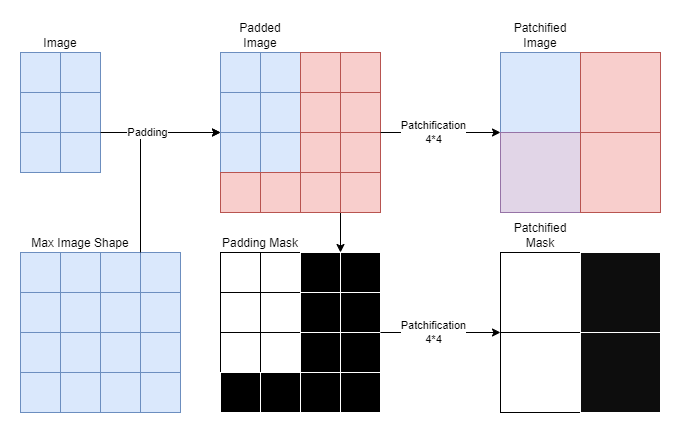
\includegraphics[width=5.0cm]{images/Design/Padding_Masking.png}
    \label{fig:padding_masking}
    \caption{Visualization of the Patching and Padding mechanisms}
\end{wrapfigure}
When an image is too small for the decoder, it is padded to be exactly \(96 \times 96\) pixels wide. When applying the padding, the image is copied into an empty array. This array has the value 1 for every pixel of the original image and 0 for every pixel of padding (respectively black and white in the figure \ref{fig:padding_masking}).\par
The creation of this mask allows the same patching transformation to be applied on both images. The image's patches will be transformed into embedding into the first transformer layer, whereas the padding image's goal is to apply a mask to the patches embedding into the first attention layer. The patches of pixel masks are reduced to a single boolean value to transform the pixel masking to a patch masking as the MHSA has no notion of pixels. The reduction aims to not lose any information from the image; as such, patches that contain at least a single pixel of original image are considered unmasked, and only the patches full of padding pixels will be masked. Such ambiguous patches are shown in the figure \ref{fig:padding_masking} where the bottom left patch is composed of two padding and two image pixels - in such case, the whole patch is unmasked.

\subsection{Layer normalization}
One difference from this implementation compared to the likes of ViT and Attention is All You Need is the location of the normalization layers. 

\begin{wrapfigure}{r}{5.0cm}
    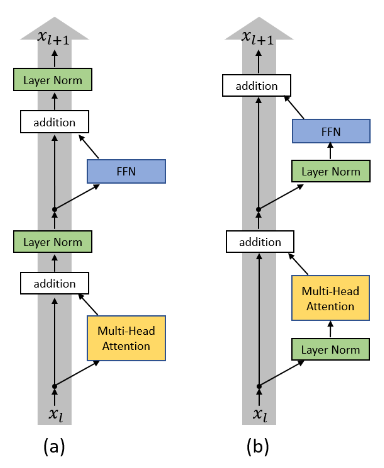
\includegraphics[width=5.0cm]{images/Design/pre-norm_layers.png}
    \label{fig:pre-layer_norm}
    \caption{Comparison of the Post and Pre-Layer normalization}
\end{wrapfigure}

On these models, the normalization layers happen after each major residual layer: MHSA and FFN. Early implementations of our architecture with the normalization layers after the main layers suffered from vanishing gradients in the latest layers. Works on normalization such as \textit{layer normalization in the transformer architecture} \cite{xiong2020layernormalizationtransformerarchitecture} hint at the post-normalization being subject to instability due to the large gradients of the previous layers and proposes a simple architecture tweak that reduce the impact on the training, especially in the early phases: pre-normalization layers.\par
Our architecture apply pre-normalization - meaning that the inputs to each major layer is passed through an initial LayerNorm as is demonstrated in the figure \ref{fig:pre-layer_norm}. The residual connection is added to the result of said layer, meaning that it does not go through the LayerNorm and allows for an easier flow of gradient through the model. This empirically helps stability, especially when multiple layers are serially chained. \\

\subsection{Causal mask}
Causal masking is used in the decoder to prevent the computation of a token's attention on future non-generated-yet tokens. This is important during training and inference, as the model shall not learn to use future tokens that are never available at inference time. The causal mask for sequence prediction is typically in the form of a triangle matrix with the upper part fully masked.\par

\begin{wrapfigure}{l}{5.0cm}
    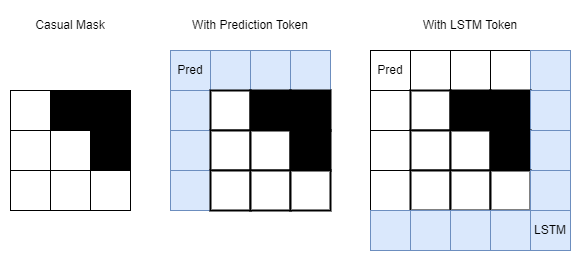
\includegraphics[width=5.0cm]{images/Design/causal_mask.png}
    \label{fig:causal_mask}
    \caption{Overview of the causal masks}
\end{wrapfigure}

Two of the structural parameters of our model use an additional token added to the target sequence. The figure \ref{fig:causal_mask} shows the three possible resulting causal mask in a sequence of length 3: In the first case without any additional tokens, the standard upper triangle matrix mask is used. In the second case when the prediction token is prepended to the sequence, a dimension is added to the matrix and the first vertical row is unmasked: this allows the token to attend to and be attended to by each token of the sequence. Similarly, the third matrix presents the case where an LSTM is added to the sequence. In this case, we unmask the last column and row of the matrix to allow the LSTM token to attend to and be attended by each token of the sequence.

\subsection{Losses and Metrics}
This section describes the losses and metrics used for the training and experiments. The objective of the loss is to quantize the error of the model in order to make better prediction over time whereas the metrics are used to evaluate the models on different objectives. \par
The model predicts the next coordinate to place at the end of a coordinate sequence. Ideally, the model should be able to estimate the direction and speed of the current curve described by the partial signal to output a likely next coordinate for the pen. In order to account for the need to respect speed and direction, the first loss used is the Euclidean loss. When a batch of predicted values is computed, the expected and predicted coordinates are matched in pairs and the loss is computed as the mean point-to-point Euclidean distance:
\begin{equation}
\mathcal{L}_{\text{Euclidean}} = \frac{1}{N} \sum_{i=1}^{N} \sqrt{\left( \text{pred}_{i,1} - \text{target}_{i,1} \right)^2 + \left( \text{pred}_{i,2} - \text{target}_{i,2} \right)^2}
\end{equation}
A mean reduction is used in order to keep the loss of a batch regularized regarding the size of said batch - meaning two experiments running on different batch sizes have comparable losses overall.\\

The second loss is focused on the shape of the generated signal in order to guide the model into keeping the generated handwriting image as close to possible as the original image it is looking at. We use the skeleton of both images to compute a loss value.

\begin{figure}[H]
    \centering
    \begin{minipage}[t]{0.45\textwidth}
        \centering
        
\includegraphics[width=\textwidth]{images/Design/Losses/skeleton_loss_build_1.png}
        \caption{Skeleton loss - All pixels mode}
        \label{fig:skel_loss_all_pix}
    \end{minipage}%
    \hfill
    \begin{minipage}[t]{0.45\textwidth}
        \centering
        
\includegraphics[width=\textwidth]{images/Design/Losses/skeleton_loss_lastpix_1.png}
        \caption{Skeleton loss - Last pixel mode}
        \label{fig:skel_loss_last_pix}
    \end{minipage}
    \caption{Overview of the Computation of the skeleton loss with both modes}
    \label{fig:skel_loss}
\end{figure}

Two alternative methods are designed and displayed in the figure \ref{fig:skel_loss}.\par
The first method on the left is called 'all pixels' as it considers every pixel of the generated skeleton. The pair of points composed of the last coordinate of the prediction sequence and the predicted coordinate is extracted in order to draw the newly generated line on the image. The original image is inverted to obtain a negative skeleton, from which we obtain a distance map where each pixel value is the closest distance to the skeleton. From there, this distance map is masked with the generated line to obtain an array containing the distances of the generated line to the skeleton. Lastly, in order to boost pixels that are closer to the skeleton and penalize pixels that are far from it, we reduce their distance values by applying a boost factor and raising the resulting value, making every pixel within the distance threshold to have its value reduced while having the opposite effect outside of the boosting range:
\begin{equation} \label{equation_loss_pix}
\mathcal{L}_{\text{skeleton}} = \left( \frac{\text{distances\_to\_skeleton}}{\text{boost\_factor}} \right)^2
\end{equation}
The second method on the right is called "Last pixel" as it considers only the pixel being currently generated. In this mode, the distance map is computed from the generated pixel and masked with the original skeleton. The closest distance on the resulting distance map represents the closest point of the generated pixel to the skeleton, and represents the loss function with the boosting shown in expression \ref{equation_loss_pix}. It is easier to obtain better loss in this mode by focusing the last pixel to always be on the original image skeleton, but it is more aligned with the Euclidean loss in terms of scale as the Euclidean distance of a single point on the image is considered.\par
The skeleton loss does not behave correctly when the model generates very far coordinates, as is typically the case during the warm-up stage. To reduce the prevalence of this loss value in the early stages of training, the expected coordinates are clamped to fit within the bound of \([0; 2 \times max\_image\_shape]\).\par
The End Of Signal token that all signals are appended with and that the model must generate in order to instruct the model to stop is in the form of the \([-1,-1]\) coordinates. This EOS token is recognized by the image generation and never added to the actual skeleton. Generating an EOS token would always lead to very bad skeleton loss with the creation of a line going to this EOS, preventing the model from learning to stop a signal. Therefore, if the next token to predict is an EOS token, the skeleton loss for that pixel is automatically excluded.\\
The total loss of the model is a weighted combination of both losses: 
\begin{equation}
\mathcal{L}_{\text{total}} = \frac{w_{\text{Euclidean}} \cdot \mathcal{L}_{\text{Euclidean}} + w_{\text{skeleton}} \cdot \mathcal{L}_{\text{skeleton}}}{w_{\text{Euclidean}} + w_{\text{skeleton}}}
\end{equation}
This allows different models with different weights to be comparable to an extent.\\

The problem of the losses is that they evaluate the capacity of the model to predict a coordinate from the "perfect subsequence" extracted from the ground truth online signal. The end goal of the model is to be able to entirely generate the online signal from the offline image without any external help. During auto-inference, the model is fed its own predictions to continue generating the sequence, which is harder than generating one datapoint on the signal. In order to reflect that and evaluate the model on the result of the auto-inference - especially to evaluate the impact of data augmentation aimed at helping the model produce more robust coordinates with imperfect data -, two additional metrics are created. Similarly as the losses, each one targets an aspect of the signal: Speed and shape.\par

\begin{figure}[H]
    \centering
    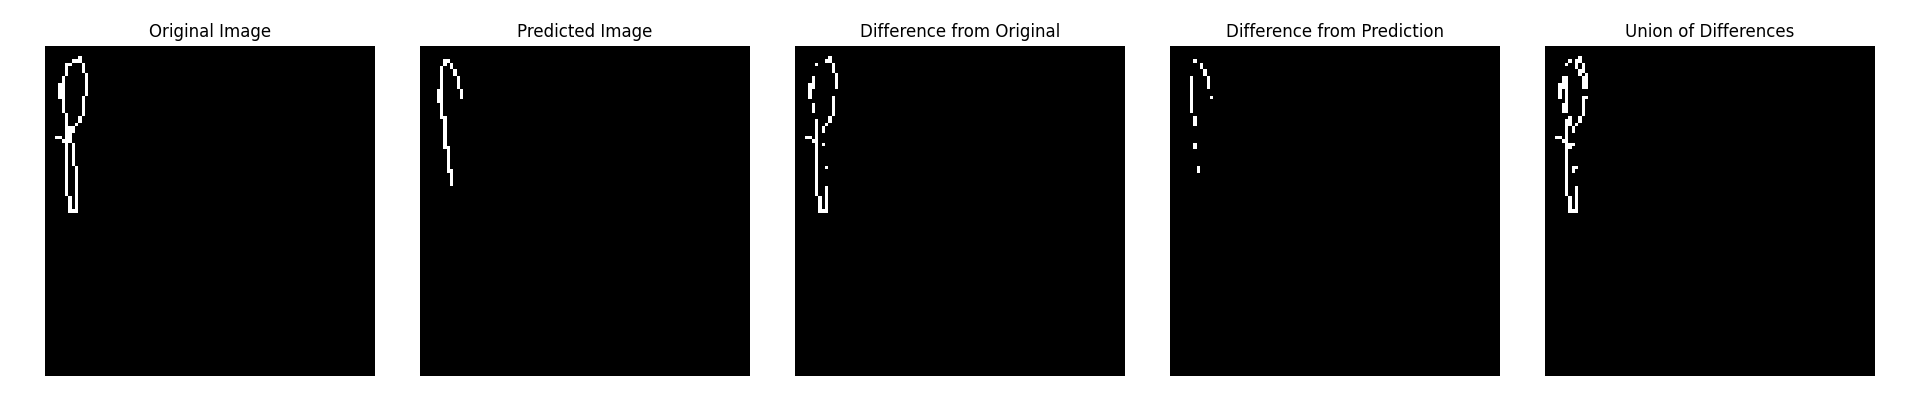
\includegraphics[scale=0.3]{images/Design/Metrics/ex_image_diff_1.png}
    \caption{Visualization of the construction of the Image difference metric}
    \label{fig:image_diff_metric}
\end{figure}

The first metrics, image diff, is focused on evaluating the produced shape by comparing the skeletons of the created and expected signals. A shown in the figure \ref{fig:image_diff_metric}, the two original and predicted images are compared. The following \(+\) and \(-\) operations are in the context of image arithmetic and are applied pixel-wise and have protection against underflow and overflow.\par
Firstly, the third image is computed by getting the difference between the original and predicted skeletons:
\begin{equation}
\text{diff\_orig\_pred}(x, y) = \max\big(0, \text{original\_image}(x, y) - \text{predicted\_image}(x, y)\big)
\end{equation}
This produces an image containing the pixels in the original image that are untouched by the generated skeleton. From that difference, we extract the following metric:
\begin{equation}
\text{diff\_orig} = 1 - \frac{\sum_{x, y} \text{diff\_orig\_pred}(x, y)}{\sum_{x, y} \text{original\_image}(x, y)}
\end{equation}
By summing the pixels of the difference and dividing them by the amount of pixels of the original image, the resulting value is a normalized 
coefficient in the range \([0;1]\) that represents the amount of pixels untouched by the predicted skeleton. This value is inverted to obtain the amount 
of pixels touched by the predicted skeletons.

Likewise, as shown on the image 4, the same operations are performed to compute the normalized difference between the predicted image and the original.
\begin{align}
\text{diff\_pred\_orig}(x, y) &= \max\big(0, \text{predicted\_image}(x, y) - \text{original\_image}(x, y)\big) \notag \\
\text{diff\_pred} &= 1 - \frac{\sum_{x, y} \text{diff\_pred\_orig}(x, y)}{\sum_{x, y} \text{predicted\_image}(x, y)}
\end{align}

This gives us the amount of pixels from the predicted image that are present on the original image.\par
One or the other value is not sufficient as they can be individually abused: 
in the first case, a limit model filling the whole image with points would touch every pixel from the original image whereas in the second case, 
a limit model that would only predict a single point in the skeleton would have all the predicted pixels touching the original image.\\

We compute a third coefficient that combines both by summing the union of the difference in a similar way:
\begin{align}
\text{diff\_union\_img}(x, y) = \text{diff\_orig\_pred}(x, y) + \text{diff\_pred\_orig}(x, y)
\notag \\
\text{diff\_union} = 1 - \frac{\sum_{x, y} \text{diff\_union\_img}(x, y)}{\sum_{x, y} \big(\text{original\_image}(x, y) + \text{predicted\_image}(x, y)\big)}
\end{align}
This union of difference value represents the sum of pixels that are in both signals. 
A model that predicts the perfect signal compared to the original has that value tending to \(1\). \\

The other goal of the model is to predict accurate trajectories, and especially speed of handwriting. In order to evaluate the coordinate as vectors, we choose two angles: First, we compute the point-to-point Euclidean distance between the ground truth and the predicted coordinates. The main problem is that the two vectors have no guarantee of having the same length. We restrict the signals' length to the length of the minimum signal, which is often the ground truth. Additionally, we compute the Dynamic Time Warping (DTW) that gives us the minimized Euclidean distance between the signals. The DTW gives us a better estimation of the overall difference between both signals as it takes into account all the data points of both vectors regardless of their size, however, it allows the signals to be warped and is thus slightly less informative about the respect of the speed of the predicted signal.\par

\section{Rejected features} \label{rejected_features}
Investigating for a good architecture involves a lot of exploration by trial-and-error. Despite our best efforts to find way to combine methods and create an efficient process, some of the features that were selected did not make the final cut as they were hampering the model too much or simply not justifying their addition to the model in terms of complexity. As failures are an important part of research, this section covers the rejected features.\\

Initially, the total loss was composed of a third loss: The EOS loss. The goal was to have a loss training each skill that we value for the model: The skeleton loss for the shapes, the Euclidean loss for the speeds, and the EOS loss for training to stop. We put a second MLP layer at the end of the transformer that output a single digit that represent the probability logit of stopping the signal. During the computation of a batch, the presence of EOS token was formatted into a vector, and we applied a binary Cross-Entropy loss (BCEWithLogitsLoss) between the logit and the expected presence of EOS. Instead of outputing the EOS coordinate \([-1;-1]\), the model would indicate through the logit the probability of stopping the signal. Because the EOS token was never predicted, the Euclidean loss was masked for EOS tokens - which is still done with the skeleton loss. This loss has been abandoned as most state-of-the-art transformers opt to make the model learn to output the EOS, and adding a second output layer and a third loss to answer an issue that can be side-stepped was considered inefficient.\\

In many Neural Networks and even Data science project as a whole, a regular step of pre-processing is the normalization of data. Some algorithms, such as K-NNs computing the distance between features, are very sensible to scale discrepancies within the input data. Normalizing the coordinate vectors can be done by dividing any coordinate (input and generated) by the maximum image shape: when the model learns to predict within the bound of the images, all coordinates are then between the \([0;1]\) range. An additional benefit of this normalization would be to pair it with a last sigmoid activation layer that return values in this exact range, making all prediction already within the bound of an image and potentially saving time during the training warm up.\par
In a non-normalized context, every coordinate is constrained within \([96,96]\) and the normalization layers within the model should take care of the coordinate normalization internally. The coordinates are even more constrained as a semi-pixel does not exist - the only valid positions are the discrete integer number within the \([0; 95]\) range.\par
During training, the model receives discrete values in the target sequence, but the predicted coordinates are decimal values. Although these represent invalid coordinates, they are still used to compute the Euclidean loss as the losses need to be smooth and give feedback to any change from the model. However, the discretization is applied before the skeleton computation and when ingesting the data again to ensure the model still has valid coordinates during auto-regression.\par
We did not notice any benefice during the training when comparing normalized to non-normalized coordinates at the cost of additional steps to make it work such adapting the image creation process or harder discretization during training and auto-inference. The addition of the last sigmoid layer on the coordinates have a terrible impact on the prediction as all coordinates are squashed to the extremes, making all coordinates a combination of \(0 \And 1\). The problem with having normalization and non-normalization cohabiting is that the scale of the loss is then different - from normalized to non-normalized loss - and are thus very hard to compare and would require the addition of a factor for normalized models. For these reasons, we opted to keep the architecture and process simple for this early proof-of-concept project and keep the coordinates non-normalized. \\

Lastly, during the initial analysis of data and creation of the data processing pipeline, another way of reducing outlier image with a shape above the maximum shape has been explored. \\

\begin{figure}[H]
    \centering
    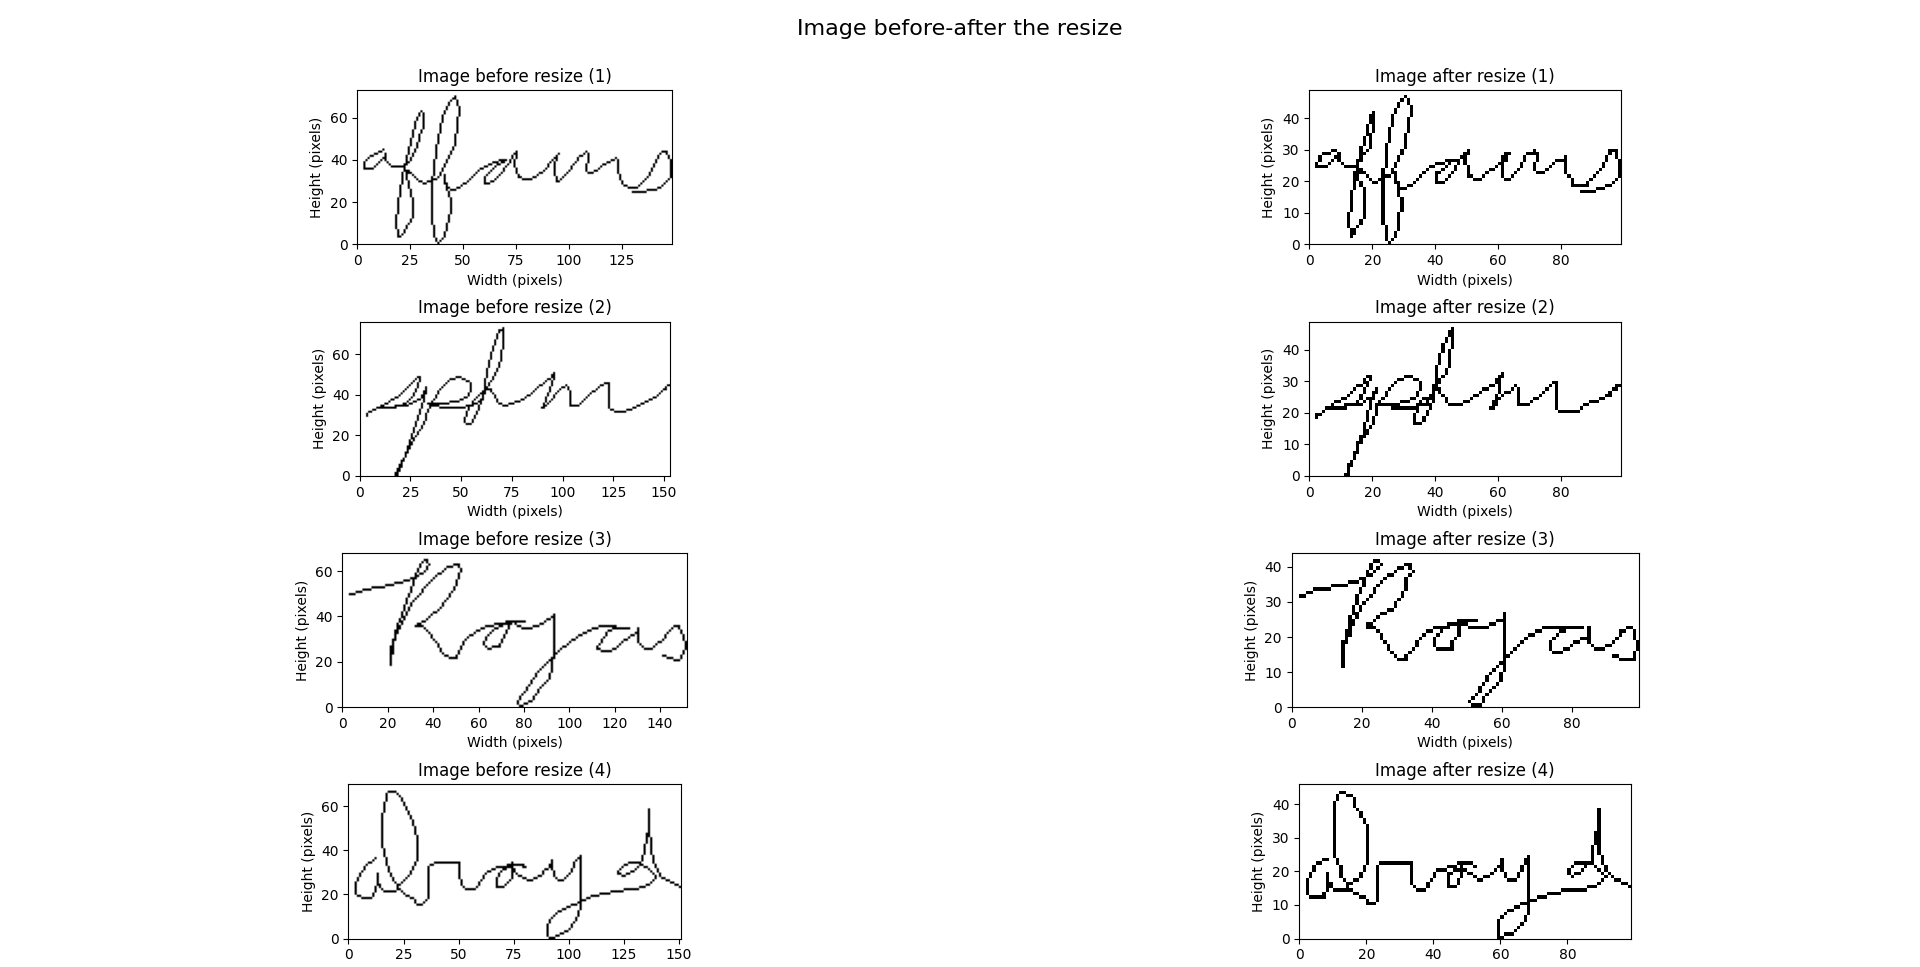
\includegraphics[scale=0.3]{images/Design/Rejected/brush_image_before_after_adapted_to_meanPlusStd.png}
    \caption{Overview of the rescaling of coordinate sequences to fit within the maximum image shape}
    \label{fig:resize}
\end{figure}

The current mechanism of image reduction cuts sequences in half until the generated images fit within the maximum image shape. The blind cuts risk creating detached sub-signals that do not have the necessary context to be correctly reproduced, making poor data for the model to learn. An alternative process for reducing the image sizes is possible via resizing: By computing a factor between the current shape of the generated image and the threshold, and keeping the width:height aspect ratio, it is possible to re-scale the coordinate vectors and obtain images that are perfectly aligned with the expectations.\par 
With this method, two thresholds coexist: The image shape threshold that is used to compute the re-scale factor, and another maximum shape threshold to exclude extreme outliers. If the rescale factor is too high, the signal can become illegible. The figure \ref{fig:resize} shows an example of four signals that are re-scaled, having final images that are about half their sizes and are still readable. But the signals are all aligned in the time and space axis to have a pixel represent the same amount of distance and two points represent the same duration in order to correctly encapsulate the speed. Resizing might respect the shape of the images, but ultimately distorts the distances and might completely prevent the model from learning acceptable speeds. Cutting the signals is considered preferable for the moment, as an imperfect but improvable method is better than loosing spatio-temporal consistency.

\chapter {Experiments}
With the design laid out, a series of experiments is conducted to analyze the trainability of the model. The first experiment verifies the impact of the structural features that were identified. Then, the second experiment focuses on the usefulness of adding data augmentation in the training dataset. The third experiment is a classical but limited hyperparameter search to identify the final best candidate for this problem. We then study the effect of training length on the model's training results, and finish by an ablation study of the LSTM module.\\

As the model is written in Pytorch, the RayTune library has been selected to run the experiments. RayTune allows for hyperparameter exploration at scale and offers a convenient way to define a search space amongst which the hyperparameter values will be sampled. Furthermore, it manages search optimization algorithms such as median pruning which reduces the number of total training to perform. For the following experiments, a training iteration is defined as a full epoch on the training dataset containing of a training and a testing loop. This yields two loss values: An average training loss and an average testing loss over the epoch. In order to avoid over-fitting and encourage generalization, the testing loss is used as the goal of the searches.\\

Running a parameter search is expensive in terms of computing power, with many training being done on suboptimal combinations. The ressources allotted to the thesis are limited with respect to the model's requirements, specifically because transformers are data-hungry by nature. To keep a reasonable trade-off between training time and relevance of the results, a single training dataset is crafted and used throughout the searches. In order to maintain consistency between the observed results and ensure reproducibility, the dataset is saved to disk, ensuring the strict separation of train/test/valid signals and guaranteeing that the same signals are used on the different trainings.\\

The training dataset is called \textit{brush\_96.96\_[train/test/valid]\_s} and is declined in three variations - un-augmented, augmented, and mix of both. This dataset is created from the BRUSH dataset, with each image kept to a 96*96 pixels format by reduction. As both datasets, BRUSH and UNIPEN, are very large, only a subset is used during these searches. The goal is to identify a relevant subset amongst the dataset in order to perform meaningful training. For the following experiment, the BRUSH signals are restricted to signals containing at least 15 coordinates after the pre-processing steps. This is done in order to avoid ingesting very small signals consisting of single / very low data point count, which lack information and are not as interesting for the model's training with regards to learning trajectories and coordinates-image correlation. 5\% of this subset's signals are taken at random, and are further separated in train/test datasets with a ratio of 0.8:0.2. Then, one thousand signals containing less than 50 datapoints and one thousand signals containing more than 50 datapoints are further sampled to constitute the validation dataset - signals that are neither in the train nor the test sets and that are used only on final model evaluation, mostly by obtaining whole predicted signals during inference, and have never been seen during training.\\

\section {Structural features}
Three structural features are defined and experimentally tested: The presence/absence of a prediction token, the utilization of a RNN in the form of a LSTM model in the decoder, and the trainability (respectively locked values) for the positional encoding added to the embedded input vectors. These experimental features aim to help the training process of the model, either by influencing its convergence speed or reaching better minimized losses. In order to test them, a full grid-search using RayTune is performed on the 8 possible combinations on 4 epochs at maximum. A median cut is used to preemptively prune poor performing combinations after a grace period of two epochs to account for eventual late start effects.\\

\begin{table}[h!]
\label{table-structural-features-results}
\caption{Results of the grid-search over structural features in terms of train and test losses}
\centering
    \begin{tabular}{ |c|c|c|c|c|c| }
        \hline
            \multicolumn{6}{|c|}{Results of the training} \\
        \hline
        \hline
            Pred. Token & LSTM & Trainable posit. & Final train loss & Final test loss & epochs\\
        \hline
        \hline
            True & False & False & 5.5195 & 4.47195 & 4\\
        \hline
            True & False & True & 5.5291 & 4.61901 & 4\\
        \hline
            True & True & True & 5.5493 & 4.63178 & 4\\
        \hline
            True & True & False & 5.5723 & 4.63778 & 4\\
        \hline
            False & True & False & 5.6019 & 4.79237 & 4\\
        \hline
            False & False & False & 5.7175 & 4.81547 & 2\\
        \hline
            False & False & True & 5.7361 & 4.94307 & 2\\
        \hline
            False & True & True & 600.0792 & 40.98933 \textit{[5.1343]} & 4\\
        \hline
    \end{tabular}
\end{table}

The table \ref{table-structural-features-results} shows the results of the grid-search over the structural hyperparameters. Each feature is represented in its on/off mode four times for a total of height experiments. Two combinations have been cut short by the median algorithm, both with no prediction token and no LSTM but with any trainable position value. This could indicate that LSTM and prediction Token being present help the convergence, as well as indicating a poor incidence of trainable position tokens. Furthermore, the last experiment has an exploding loss compared to every other. Before concluding on these data, a re-run of the exploding experiment has been tried to correct the final test loss. \\

\begin{figure}[H]
    \centering
    \begin{minipage}[t]{0.45\textwidth}
        \centering
        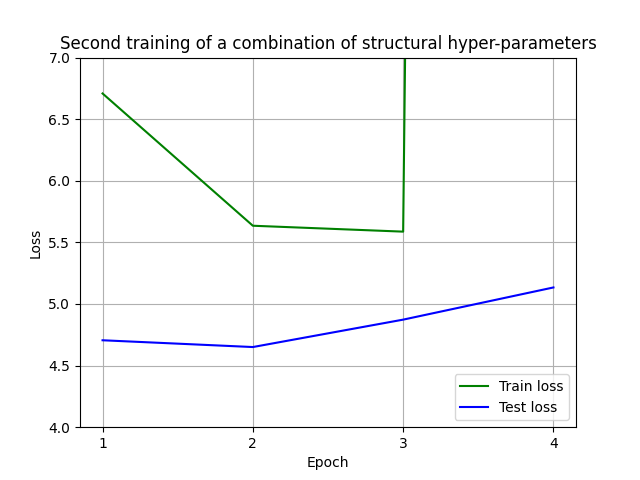
\includegraphics[width=\textwidth]{images/Experiments/structural/reworked_train_test_losses.png}
        \caption{Train-Test losses per epoch}
        \label{fig:rerun_train_test}
    \end{minipage}%
    \hfill
    \begin{minipage}[t]{0.45\textwidth}
        \centering
        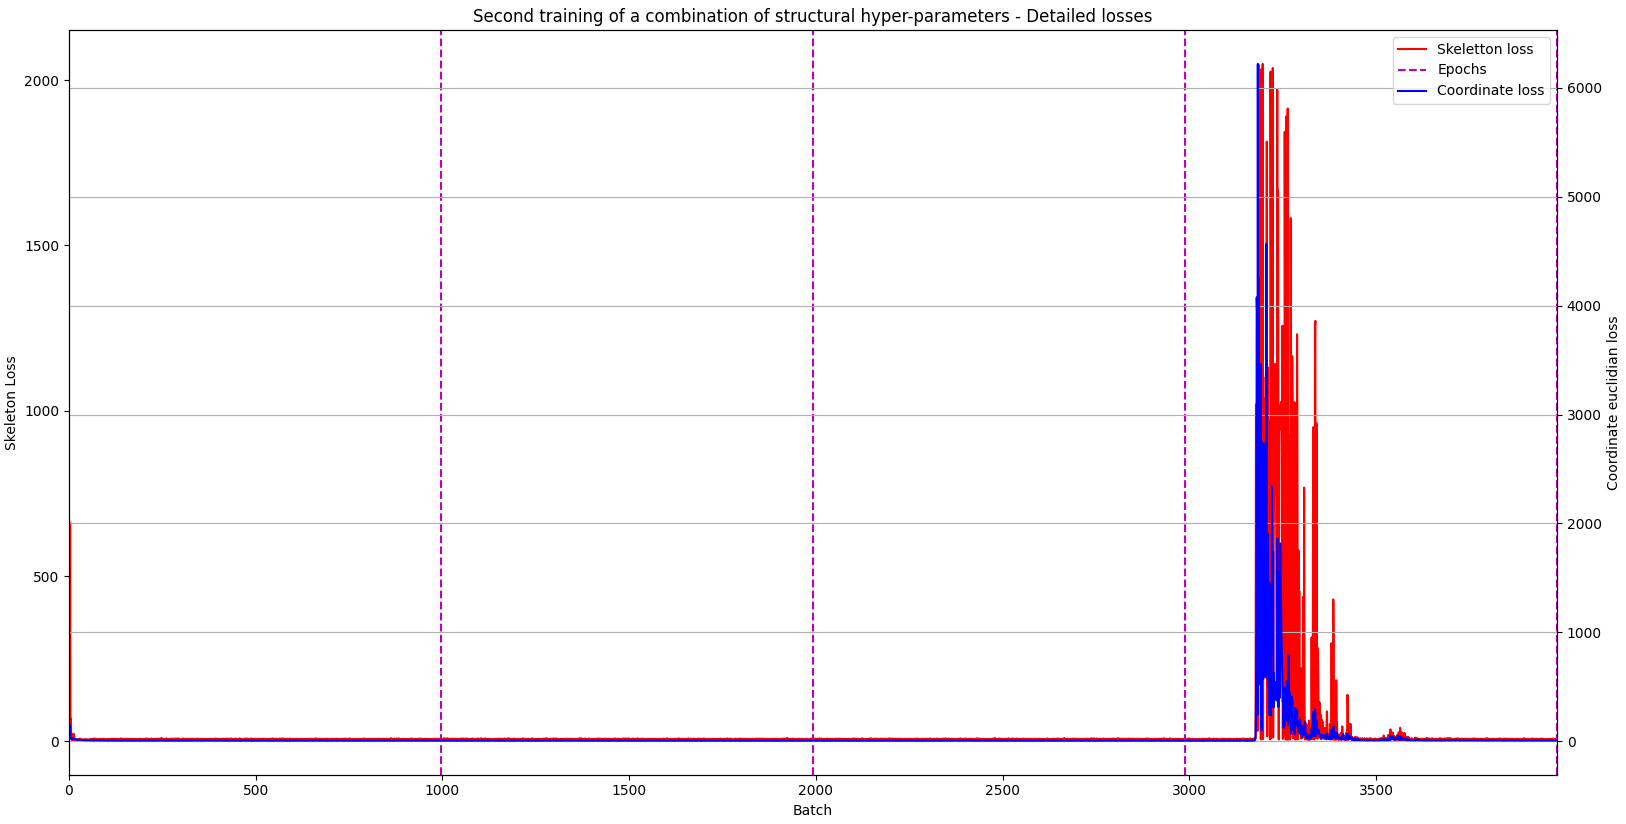
\includegraphics[width=\textwidth]{images/Experiments/structural/reworked_detailed_train_test_losses.png}
        \caption{Train-Test losses per batch}
        \label{fig:rerun_detailed_train_test}
    \end{minipage}
    \caption{Rerun of the exploding combination over four epochs}
    \label{fig:rerun_side_by_side}
\end{figure}

The results of the re-run of this combination are shown in the side-by-side graphs on the figure \ref{fig:rerun_side_by_side}. It is interesting to observe in the detailed train-test losses per batch in the figure \ref{fig:rerun_detailed_train_test} that the re-run suffered the same fate of exploding loss during the last epoch. This explosion altered the final average train loss to reach the scale of hundreds, similarly as during the initial grid-search. Although the model is capable of getting back on track after a sufficient number of batches, the test loss is still negatively impacted as shown in the figure \ref{fig:rerun_train_test}. This final test loss is added to the result table as an additional point of information, but the fact that two identical problems happened on the same combinations can be indicative of a bad mix. This might also hint at a problem of high learning rate for which reducing the value could be advised.\\

\begin{figure}[H]
    \centering
    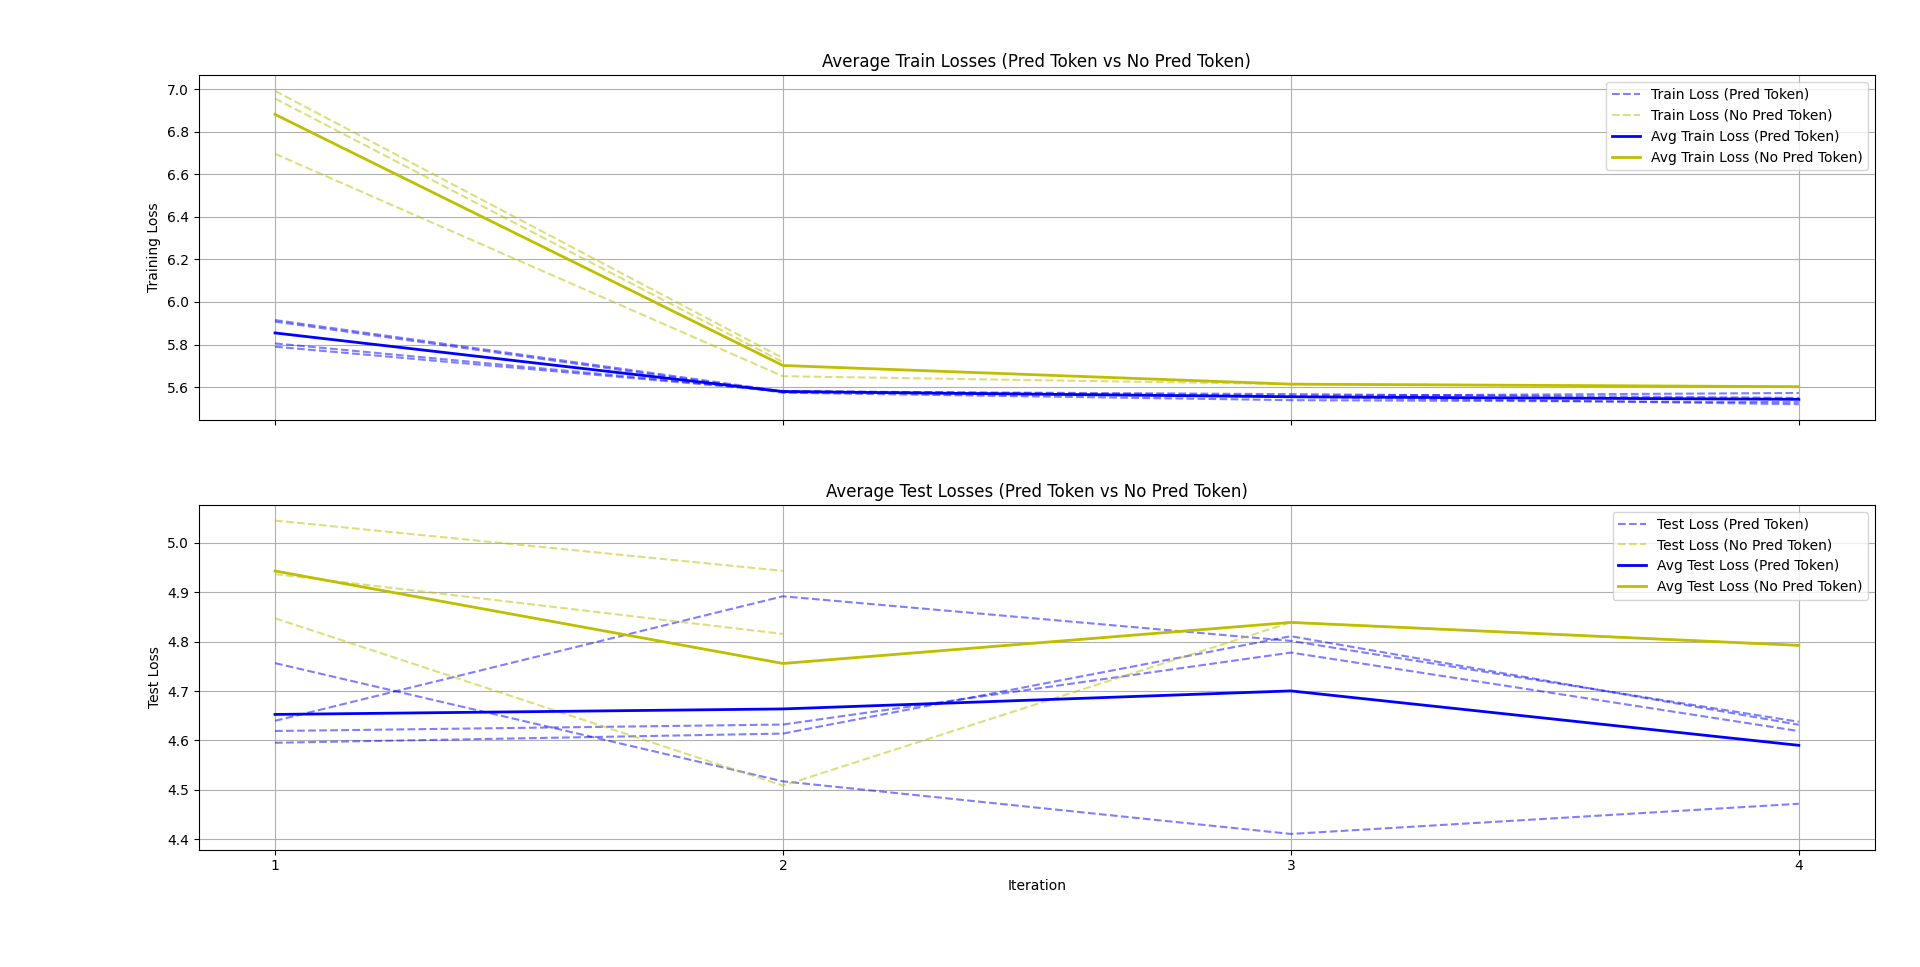
\includegraphics[scale=0.3]{images/Experiments/structural/train_test_losses_pred-token.png}
    \caption{Comparison of the model's results focused on the presence-absence of Prediction Token}
    \label{fig:results_structural_PredToken}
\end{figure}
The figure \ref{fig:results_structural_PredToken} display all the train-test losses over the four epochs with a focus on the prediction token. In yellow, the four dashed lines represent the four individual combinations with no prediction token in their structure, with the full line representing the average over the four. Meanwhile, the blue lines represent the models and their average with prediction token. \\

In the train and the test cases, it is interesting to see that the prediction token's presence seems to be a major indicator of good relative performance, as every individual model performs better than its counterpart. Additionally, two of the four remaining models without a prediction token are stopped at the first iteration as their performance was above the median of the models. The average curves also indicate a clear benefit of having prediction tokens in all cases.\\

\begin{figure}[H]
    \centering
    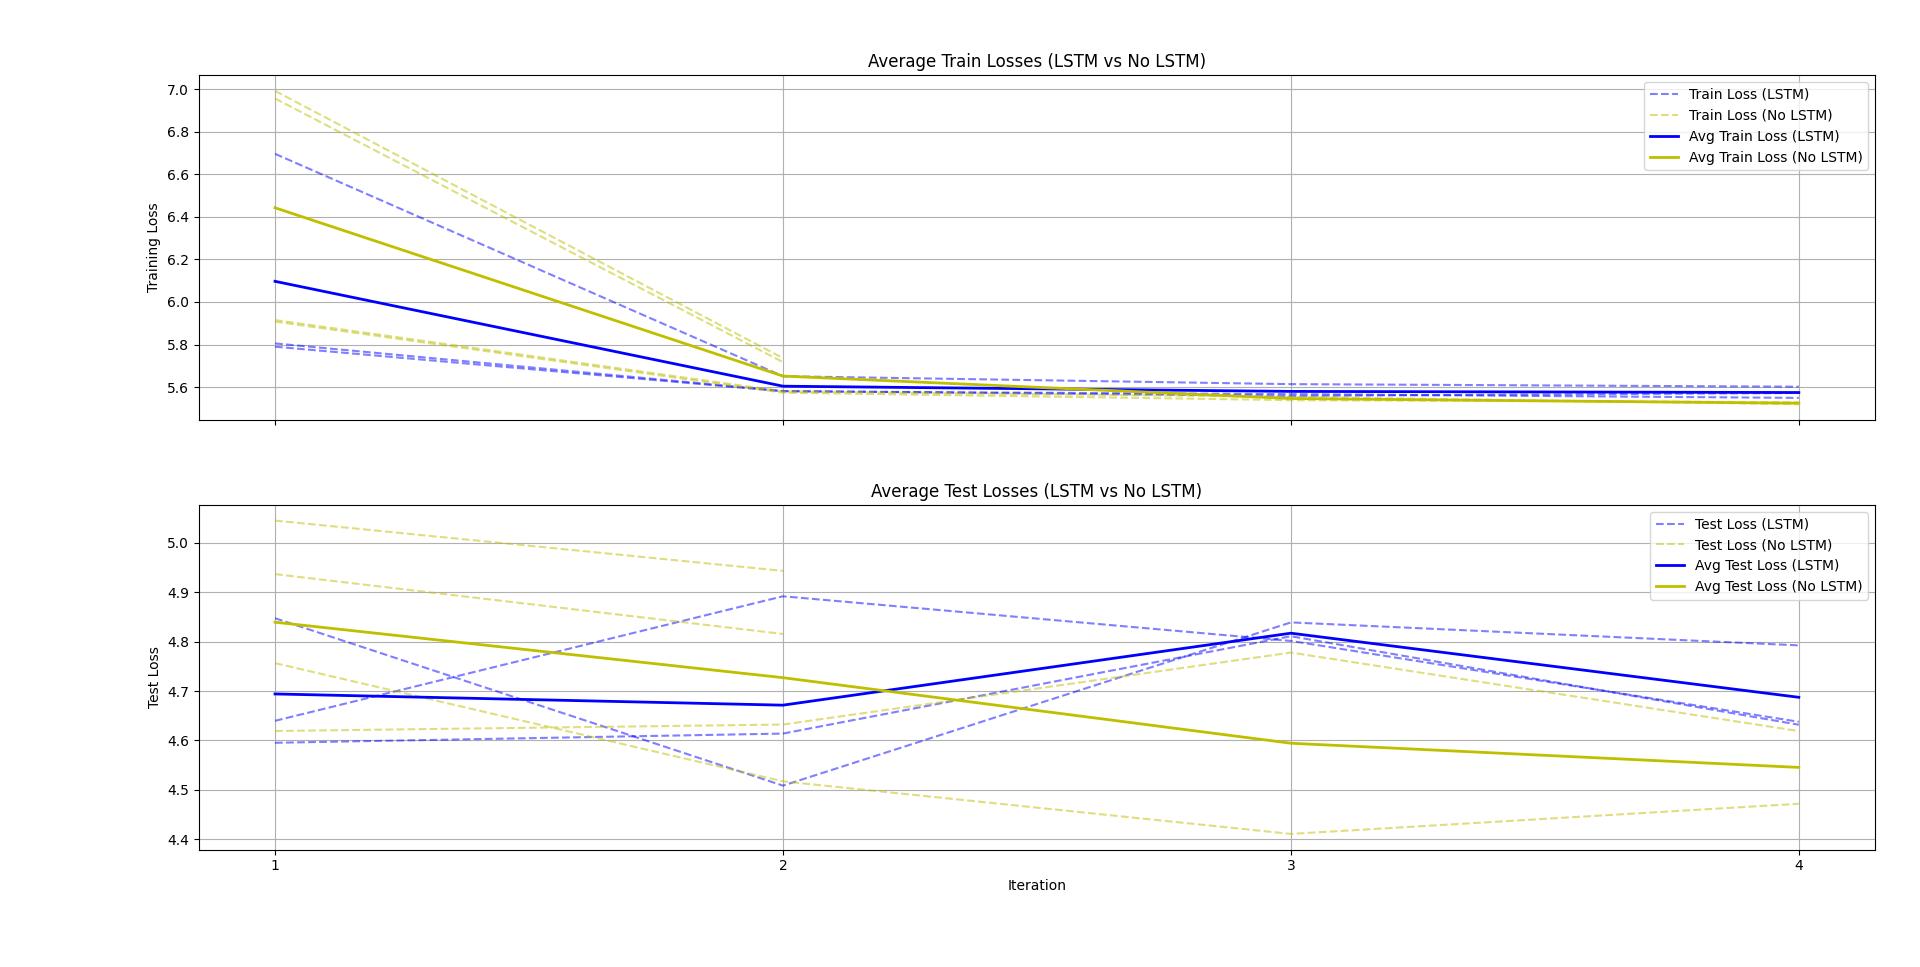
\includegraphics[scale=0.3]{images/Experiments/structural/train_test_losses_lstm.png}
\caption{Comparison of the model's results focused on the presence-absence of LSTM}
\label{fig:results_structural_LSTM}
\end{figure}

The second figure (\ref{fig:results_structural_LSTM}) presents the same presence-absence scenario focused on the LSTM. In the upper graph showing the train losses, the average with or without are very close. However, two out of the four models without LSTM are stopped at epoch two as poor relative performers. Furthermore, the bottom graph showing the test losses reveals that the LSTM models attain a faster convergence for the first two epochs while converging to the same average from the third on. However, the final loss is very close with or without the presence of LSTM. It is important to note though that with two poor performers eliminated, the average without LSTM is skewed toward its better performers. Overall, although the observations are not as overwhelming as for the presence of a prediction token, the presence of a LSTM token seems to help early convergence and produce slightly better models without being a ground-breaking innovation. \\

\begin{figure}[H]
    \centering
    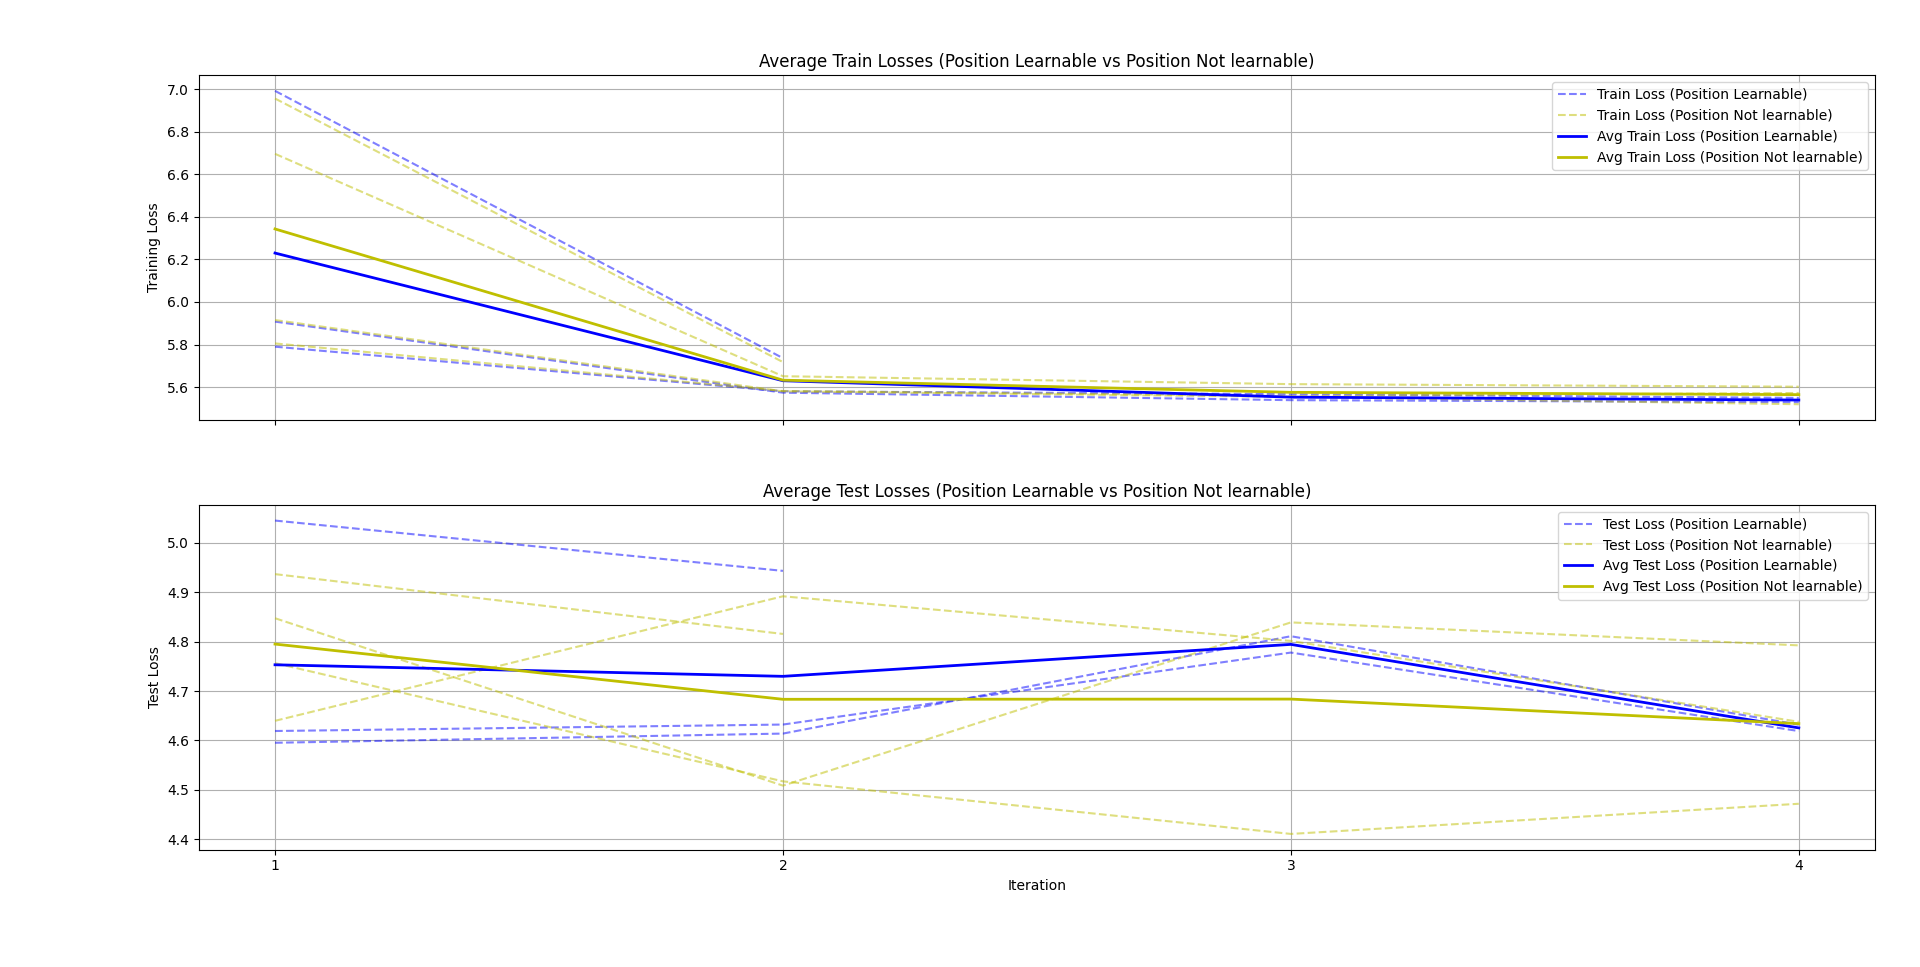
\includegraphics[scale=0.3]{images/Experiments/structural/train_test_losses_position-learnable.png}
\caption{Comparison of the model's results focused on the position tokens being learnable}
\label{fig:results_structural_posLearnable}
\end{figure}

Lastly, the figure \ref{fig:results_structural_posLearnable} shows the same experiment results focused on the positional tokens being trainable or fixed. In this case, both averages of the upper (train) and the lower (test) graphs show no strong sign of impact of the structural feature. This could indicate that having positional token learnable is neither helpful nor harmful to the model's training. However, the small nature of the dataset used (5\% of BRUSH) and the little amount of epochs could be too small to learn meaningful position tokens, whereas a longer training could reveal more usefulness of this feature. \\

The conclusion of this experiment is that prediction token shows strong signs of being beneficial to the model's training with overall better convergence over the training period. The conclusion is a bit more nuanced for the LSTM, which still shows good signs and can be investigated further. Lastly, the position token being learnable has little incidence on the training with these parameters, but it is hard to conclude on the root cause being the feature itself or the low amount of training resources during the grid search.
 
\section {Impact of augmentation}
The second experiment intends to test the addition of a data augmentation in the form of a Gaussian noise to help the model achieve better consistency of the generated signals during inference. The experimental protocol is as follows: Three models are trained. The first one only sees the original data, which predicts on the images generated by the coordinates, making a perfect match. The second model is given only noised data, meaning there is virtually little match between the coordinates and the images. Lastly, the third model is given the mix of augmented and unaugmented data.\par
The train and test losses of each model are not interesting comparison metrics as they only reflect the ability to predict the next label based on a perfect sequence. With that in mind, the unaugmented model will be favored by the perfect conditions of its training meanwhile the mixed model will be favored as it has twice the amount of data during training.\par
The comparison will be structured around the quality of the generated signals during inference on the same validation dataset containing \(2000\) signals, of which half are considered "small" and half are "large", with a respective length \(15 <= length <= 50\) and \(50 <= length\). The first point of comparison is the general length of the generated signal as the models tend to have a hard time stopping. The second point of comparison are the global evaluation metrics - DTW, Euclidean distances, and image differences - to compare the three models.

\begin{figure}[H]
    \centering
    
\includegraphics[scale=0.35]{images/Experiments/Augmentations/length_distribution.png}
    \caption{Length distribution of the expected and predicted signals with different augmentation during training}
    \label{fig:Distribution_expected_predicted_signals}
\end{figure}

The distribution of the generated signals in the figure \ref{fig:Distribution_expected_predicted_signals} shows the lengths' distribution of the 2000 signals of the ground truth and each of the three models: Unaugmented, Augmented, and Mixed. The ground truth in green appears three times as a reference: Once for the small signals, once for the large signals, and once for the complete validation dataset.\par
Following the ground truth, the next three distributions represent the generated signal with an artificial cut of the generation when the predicted signal reaches the length of the original signal and labeled "Early Stop". The following three distributions represent the generated signal with twice the threshold for the artificial cut, letting a chance to the model to stop the signal using the EOS token, and is labeled "Natural Stop". As it was observed that model stopping is a hard-learned feature, we add another artificial cut once a number of consecutive signals are identical as an indication that the model is not able to predict anymore. \par
In all cases, the 'Early stop' signals have the exact same distribution as the ground truth, indicating that the models are never stopping the generation of the signals themselves before the signal length is reached. However, the Natural stops have a bit more variation. For the small signals, all three models run for the same duration and the stop is not instructed. For the large signals, a significant difference is observed, with the augmented dataset stopping earlier than the unaugmented, and the mixed dataset having an even smaller distribution. The same observation applies to the analysis of the complete dataset where the predicted signals distributions are smaller across the augmented and mixed models.

\begin{figure}[H]
    \centering
    
\includegraphics[scale=0.35]{images/Experiments/Augmentations/distances_list_all_models_small_signals.png}
        \caption{Distance results (DTW, Euclidean) of the models on small signals}
        \label{fig:distances_small}
\end{figure}

The distance results on the small signals plotted on the figure \ref{fig:distances_small} shows the DTW distances on top and the point-to-point distances on the bottom.\par
The DTW distances have a similar observation on early or natural stop: The overall values of the DTW is larger for the unaugmented model and gets better with augmented and mixed models. Although the medians are very close, we observe an amelioration of the third quartile, indicating that there are fewer signals that are very far from the original skeleton.\par
As the Euclidean distances are computed point-to-point, the computation stops once the first EOS is reached. As a result, the early and natural stops distances are very similar. Overall, we notice no real distinction between the different augmentations.

\begin{figure}[H]
    \centering
    
\includegraphics[scale=0.35]{images/Experiments/Augmentations/distances_list_all_models_large_signals.png}
        \caption{Distance results (Euclidean, DTW) of the models on large signals}
        \label{fig:distances_large}
\end{figure}

The distances over the large signals are plotted on the figure \ref{fig:distances_large}. The large signals are longer and more complex to follow along, meaning there are more requirements on the models to obtain good signals from these images.\par
The addition of augmentation result in an increasing overall distance to the original large signals. 
Although the Q1 and Q2 are similar, the third quartile becomes larger, meaning we have a larger trail of signals of lower quality. \\

The distances are only one side of the coin as they inform us only of the capacity of the model to stick to the original signal, but different explanations could result in the slight loss of performance for augmented models. For example, different prediction speeds will induce a latent variation of the distances without impacting the shape of the image. We also observe that the augmentation of the point-to-point distance does not correlate with an augmentation of the DTW distance for the mixed model.

\begin{figure}[H]
    \centering
    
\includegraphics[scale=0.35]{images/Experiments/Augmentations/diff_list_all_models_small_signals.png}
        \caption{Difference on the skeletons of the models on small signals}
        \label{fig:image_diff_small}
\end{figure}

We plot the difference of the skeletons on the figure \ref{fig:image_diff_small}. 
This score represents the proportion of matching pixels from the original signals that have been predicted, the proportion of predicted pixels that exist in the original image, and lastly, the percentage of matching pixels over all the pixels of both.\par
The same observation can be done for all small signals: The unaugmented dataset has a lower matching of images over all metrics, followed by the augmented and the mixed, 
the latter having a close upper hand. For example, the matching pixels of the union image of the unaugmented model has a median below \(20\%\), 
which goes up by almost \(10\%\) for the augmented and mixed models. 
Overall, the mixed model performs slightly better than the augmented model and both have a better matching ratio than the unaugmented model.

\begin{figure}[H]
    \centering
    
\includegraphics[scale=0.35]{images/Experiments/Augmentations/diff_list_all_models_large_signals.png}
        \caption{Difference on the skeletons of the models on large signals}
        \label{fig:image_diff_large}
\end{figure}

Lastly, the ratios over large signals plotted on the figure \ref{fig:image_diff_large} reflect a little less variation, although on all but one case, the observation is the same: 
the augmentation performs slightly better than the unaugmented model, and the mix of both have a higher matching. The only exception is for the difference from the original image
where the mixed dataset has a slightly worse matching ratio and was unable to stick to the original skeleton. \\

The conclusion of the experiment is that the addition of the augmentation itself is beneficial, especially for the predicted image skeletons sticking better to the originals signals, although we observe better results when the model is able to train with both the "perfect" (unaugmented) and the noised signals. 
Although this doubles the size of the dataset, the results are better and the mix of both is consistently better than one or the other.

\section {Best candidate}
The third experiment aims to find the best candidate model by doing a hyperparameter exploration. As discussed in the design section, the architecture of the model has a lot of parameters
which can be adjusted.

\begin{table}[H]
    \centering
    \begin{tabular}{|p{3cm}p{4cm}p{8cm}|}
    \toprule
        \textbf{Hyperparameter} & \textbf{Type} & \textbf{Rationale}\\
    \hline
        \multicolumn{3}{|c|}{Structural hyperparameters} \\
    \hline
        Prediction Token & True - False & Addition of a prediction token in the decoder, modification of last layer MLP \\
        LSTM  & True - False & LSTM model guide the prediction by adding its last hidden layer computed on the target sequence \\
        Learnable tokens & True - False & Positional tokens are learnable instead of fixed \\ 
        \hline
            \multicolumn{3}{|c|}{hyperparameters} \\
        \hline
        Image Size & Shape \([w,h]\) & Sensible size for the maximum image shape \\ 
        Patch Size & Shape \([w,h]\) & Sensible size for the patches, ideally divides Image size, related to hidden dim \\
        Hidden Dimension & Unsigned Integer & Dimensionality of the tokens inside the transformer, ideally related to image / patch size \\
        Context length & Unsigned Integer & Number of datapoints of context given to the decoder from the target sequence \\
        LR & Usually \([1e-3; 1e-5]\) & Starting learning rate of the model \\
        Batch Size & Usually \(2^n\) & Number of images computed by batch, impact performances and results \\
        Heads & Unsigned Integer dividing \(D_{hidden}\) & Number of heads in the Encoder - Decoder \\
        Layers & Unsigned Integer & Number of layers for the Encoders-Decoders \\
        FFN activation functions & Activation Function (Relu, Sigm...) & Activation functions in the Encoder-Decoder FFNs \\
        FFN expansion ratio & Unsigned integer k\([1-N]\) & Expansion ratio in the FFNs of the Encoder-Decoder \\
    \hline
        \multicolumn{3}{|c|}{Data-related hyperparameters} \\
    \hline
        Loss weights & Pair \((W_{Eucl}, W_{Skel})\) & Weight given to each loss in the computation of the total loss \\
        Skeleton loss mode & LastPix or SumPix  & Sumpix considers all pixels generated, LastPix computes the distance of the last pixel \\
        Gauss. STD + Mean & Pair of decimal value & parametrization of the Gaussian Noise \\
    \bottomrule
    \end{tabular}
    \caption{Summary of all hyperparameters available for the model's architecture}
    \label{table:summary_all_hyper_parameters}
\end{table}

The full list of hyperparameters is detailed in the table \ref{table:summary_all_hyper_parameters}. They can be decomposed in three parts: The structural hyperparameters that are already 
tested and are excluded from this search, the regular hyperparameters, and the data-related parameters.\par
Excluding the three structural parameters, 13 hyperparameter with a varying degree of ranges can still impact the performance of the models. Unfortunately, this represents too many combinations.
Therefore, we apply a selection to restrict the number of trainings to test.\par
The Image size, Patch size and hidden dimensions are fixed to \(96 \times 96\), \(16 \times 16\) and \(D_{hidden}=256\). These represent consistent values where the image sizes are adapted to the data and 
the patch size and hidden dimension allow the information to be flowing without dimensionality reduction. Similarly, the context length is fixed to \(50\) prior coordinates per prediction.\par
The batch size is fixed to \(512\) as this represents the computational limit of the GPU used to run the search, maximizing its utilization.\par
The Skeleton mode is fixed to LastPix and the Gaussian noise is paramatrized to a mean and standard deviation of (0,1) as a baseline that has low chances of impacting the training negatively.
The FFN activation function and expansion ratios are excluded from the search and fixed to LeaKyRelu and \(4\) as standards.\par
The search is used to explore the Learning rate, the number of Heads, the number of layers, and the pair of weights as they are suspected of having a great effect on the final results.

\begin{table}[H]
    \centering   
    \caption{Repartition of the dimension per head}
    \begin{tabular}{ |c|c|c|c|c|c|c|c| }
        \hline
            \multicolumn{8}{|c|}{Repartition of dimensional subspace per head} \\
        \hline
        \hline
            Number of heads & 2 & 4 & 8 & 16 & 32 & 64 & 128 \\
            Dimension per head & 128 & 64 & 32 & 16 & 8 & 4 & 2 \\
        \hline
    \end{tabular}
    \label{fig:head_dimensions}
\end{table}

The number of Heads is selected as an important parameter as each attention token is subdivided equally between the number of heads. 
The table \ref{fig:head_dimensions} shows the dimension of the sub-token given per head. Attention Is All You Need has 8 heads for a \(D_{hidden}\) of \(512\), meaning each head
occupies a dimensional subspace of \(64\). In our case, with a \(D_{hidden}\) of \(256\), this would equal to 4 attention heads.\par

\begin{table}[H]
    \centering
    \caption{hyperparameter selected for the Search}
    \begin{tabular}{ c|c }
        \hline
            Hyperparameter & Values \\
        \midrule
            Learning Rate & \(1e-3, 1e-4, 1e-5\) \\
            Number of heads & 4, 8, 16 \\
            Number of layers & 6, 12 \\
            Losses Weights & \((0,1), (1,0), (1,1), (1,1), (1,3), (3,1)\)\\
        \hline
    \end{tabular}
    \label{table:head_dimensions}
\end{table}

The parameters selected for the search are listed in the table \ref{table:head_dimensions}.\par
The Learning rates are sampled amongst the usual range of learning rates, knowing that lower learning rates are usually preferred for transformers, specifically given the exploding losses
that can occur during the training.\par
The number of heads is expected to be the same on the encoder and the decoder, although that is not a strict requirement. We test three values starting from a baseline of 4.\par
To limit the number of tested combinations, two possible number of layers are selected, once again assuming a uniform number of layers across encoder and decoder: 6 for the low value, 12 for 
the high value. A higher number of layers could allow the model to extract more complex patterns from the data, but is not guaranteed and can cause harder propagation inside of the model.\par
Lastly, we test three configuration of the losses combinations: Two all-or-nothing, two equilibrium, and two that heavily favor one or the other. \par
The search is performed as a grid-search over all parameters making for a total of 108 combinations. \\ 

\begin{table}[h!]
    \centering
    \caption{Top 10 Results of Hyperparameter Search}
    \label{tab:top_results}
    \begin{tabular}{|c|c|c|c|c|c|}
        \hline
        Learning Rate & Weights & Heads & Layers & Train Loss & Test Loss \\
        \hline
        0.0001 & (1, 0) & 4 & 12 & 3.821 & 3.774 \\
        0.0001 & (1, 0) & 16 & 6 & 3.842 & 3.810 \\
        0.0001 & (1, 0) & 8 & 6 & 3.842 & 3.831 \\
        0.0001 & (1, 0) & 8 & 12 & 3.823 & 3.886 \\
        0.0001 & (1, 0) & 4 & 6 & 3.893 & 3.890 \\
        0.0001 & (3, 1) & 4 & 12 & 4.620 & 4.055 \\
        0.0001 & (1, 0) & 16 & 12 & 3.791 & 4.058 \\
        0.0001 & (3, 1) & 8 & 12 & 4.600 & 4.059 \\
        0.0001 & (3, 1) & 16 & 12 & 4.593 & 4.088 \\
        0.0001 & (3, 1) & 8 & 6 & 4.633 & 4.104 \\
        \hline
    \end{tabular}
\end{table}

\begin{figure}[H]
    \centering
    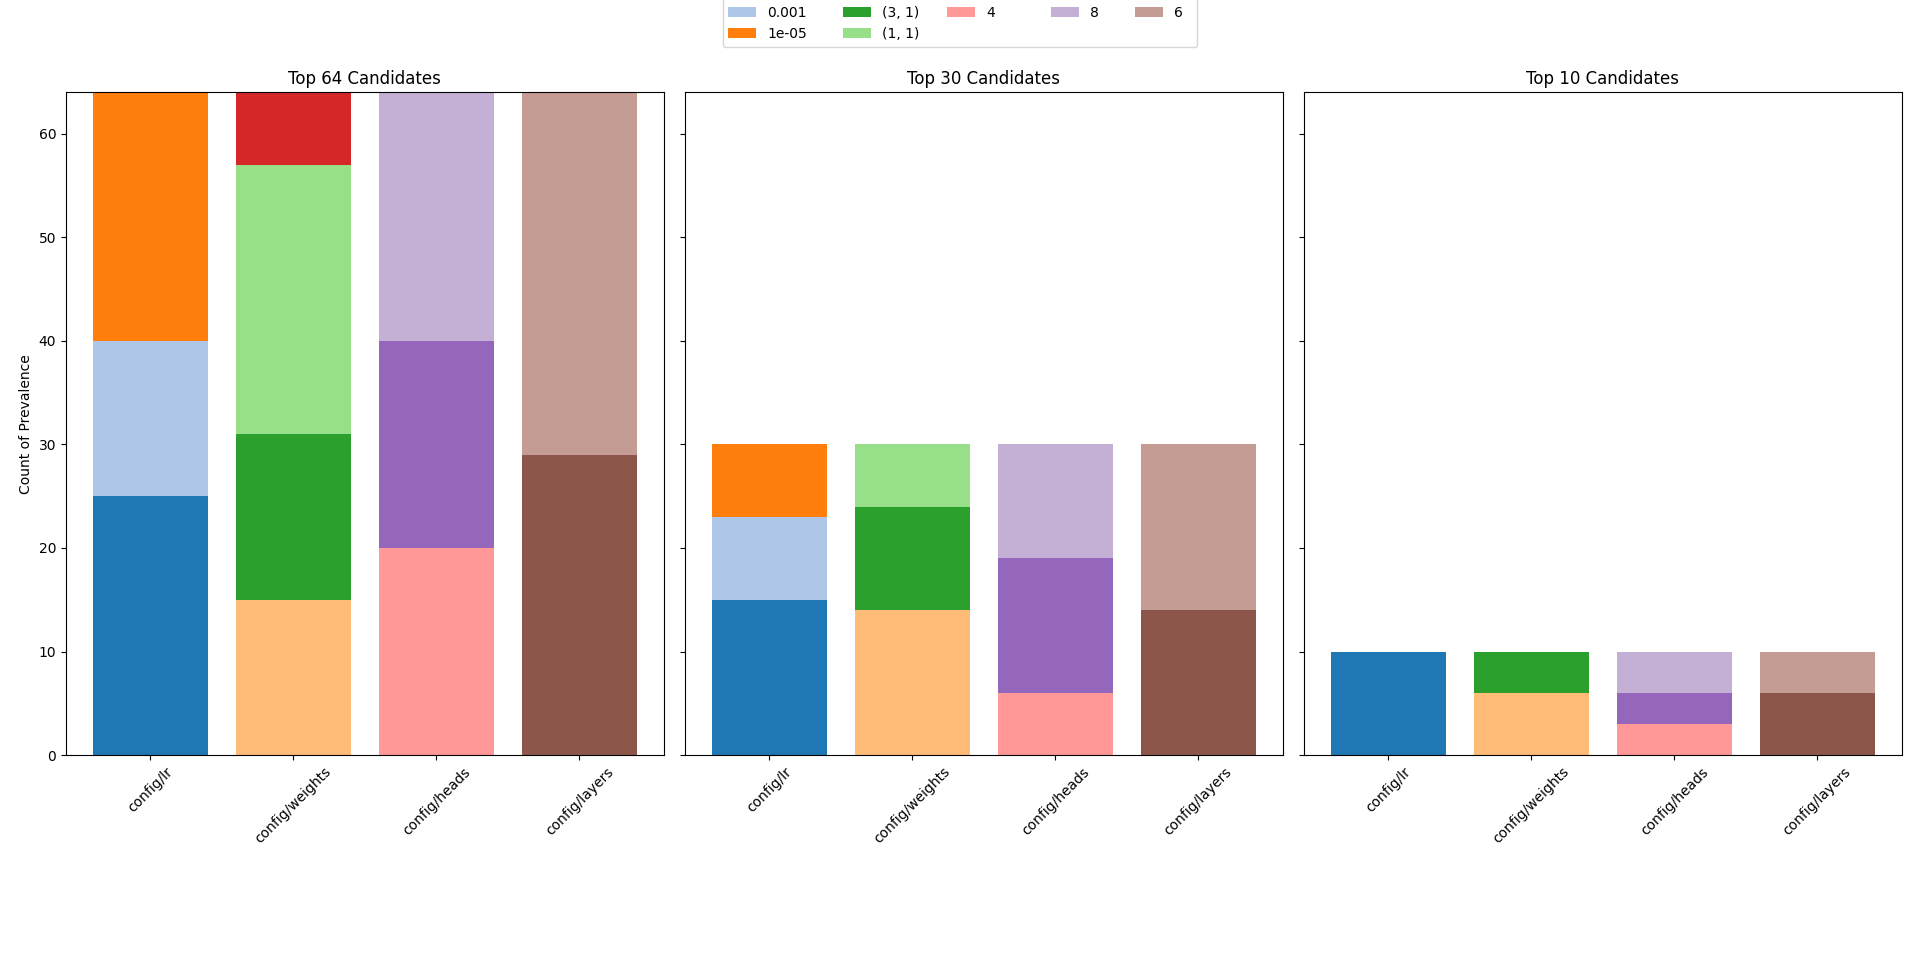
\includegraphics[scale=0.33]{images/Experiments/parameters/results_prevalence.png}
        \caption{Prevalence of hyperparameter values in the top 64, 30, 10 models}
        \label{fig:prevalence_tops}
\end{figure}

The results of the hyperparameter search are displayed in the table \ref{tab:top_results} for the top10 models, 
and in the figure \ref{fig:prevalence_tops} showing the Top 64 - 30 - 10 candidates.\par
In both cases, some parameters values seem to have a lot of impact. For example, the learning rate is majorly dominated by the value \(1e-4\) that overshadows
its alternatives. \par
The weight prevalence is very interesting as two combinations take most of the better models: \((1,0)\) and \((3,1)\) - the former being all Euclidean distance and no Skeleton and the latter being majorly Euclidean with a little skeleton loss. The Euclidean seems to favor good learning, although it is important to state that while both losses are
on the same scale, the fact that the test loss is the comparison metric can skew this result in favor of a loss that has a lower average value. Nevertheless, the presence
of mixes of \((1,1)\) and \((3,1)\) in the top64 proves that the scale of the losses alone might not be the issue that the presence of some skeleton loss is 
beneficial for training, with an optimal trade-off favoring the Euclidean distances.\par
The results are more mitigated for both the number of layers and head, with all the values still being present in the top10 and no strong indicator that either value
is better. In case of equal impact, the lower complexity can be favored as it saves on computations and reduces the risk of over-fitting.

\begin{table}[h!]
    \caption{Average ranks for each configuration, sorted by rank within each category.}
    \centering
    \begin{tabular}{cc}
    \toprule
    \textbf{Configuration} & \textbf{Average Rank} \\
    \midrule
    \multicolumn{2}{l}{\textbf{Learning Rate (lr)}} \\
    0.00010 & 43 \\
    0.00001 & 55 \\
    0.00100 & 65 \\
    \midrule
    \multicolumn{2}{l}{\textbf{Weights}} \\
    (1, 0) & 29 \\
    (3, 1) & 32 \\
    (1, 1) & 50 \\
    (1, 3) & 68 \\
    (0, 1) & 98 \\
    \midrule
    \multicolumn{2}{l}{\textbf{Heads}} \\
    16 & 52 \\
    8 & 53 \\
    4 & 58 \\
    \midrule
    \multicolumn{2}{l}{\textbf{Layers}} \\
    6 & 52 \\
    12 & 57 \\
    \bottomrule
    \end{tabular}
    \label{tab:average_ranks}
\end{table}

Finally, the table \ref{tab:average_ranks} regroups the hyperparameter by their average rank amongst the 108 combinations. A parameter above the median (54) 
can be judged beneficial while a parameter below is to be avoided.\par
The observations made in the previous analysis stand for learning rate and weights, with \(1e-4\) being at average rank 43 and the second parameter being at rank 55.
Similarly, the weight pairs ordered by rank show a clear focus on Euclidean loss. \par
All the values for Heads and Layers gravitate towards the median with \(52,53,58\) for the heads and \(52,57\) for the layers. The values of 
4 heads and 12 layers performs slightly below their contenders, meaning they can be excluded, as well as the 16 heads where the cost in complexity is 
not worth the very little gain.\\

Overall, we found a very high impact of learning rate and weight combination of the results of the models while the number of heads and layers had a lower impact.
The best candidate for this task is a model with a LR of \(1e-4\), a weight favoring the Euclidean loss, \(8\) attention heads and \(6\) layers.\par
More in-depth analysis could assess the impact of other hyperparameter as well as their combinations, such as FFN tuning, Gaussian noise, or skeleton loss mode.
Furthermore, it would be interesting to run such an analysis on more than four epochs as the limited training time can give an advantage to some values (lower number of layers, 
lower number of heads).

\section{Impact of Training size}
All models previously tested have been run on the small dataset on four epochs. The small dataset has a length of \(1'000'000\) datapoints divided
across \(250'000\) signals. As the signals are randomly sampled from BRUSH and represent \(5\%\) of the dataset without any stratification, it is possible
that some characters or writers remain unseen. Additionally, a loss plateau has never been hit and the models never showed a sign of decreased learning in 
the four epochs that they trained on. This experiment aims to train the best candidate determined in the previous one on more data to investigate
the capacity of this model to go beyond its current results.\par
Firstly, the model is trained on the small dataset for 30 epochs to investigate the learning capability of the model. Then, the model is trained on a 
medium BRUSH dataset composed of \(20\%\) of the dataset for 8 epochs to investigate the gain of seeing more different signals.\par
This medium dataset is composed of \(4'000'000\) datapoints divided amongst \(990'000\) signals. 
The 30 epochs on the small dataset represent a total of \(30M\) datapoints against \(32M\) datapoints for the 8 epochs of the medium dataset, representing
an almost equivalent training.

\begin{figure}[H]
    \centering
    \begin{minipage}[t]{0.45\textwidth}
        \centering
        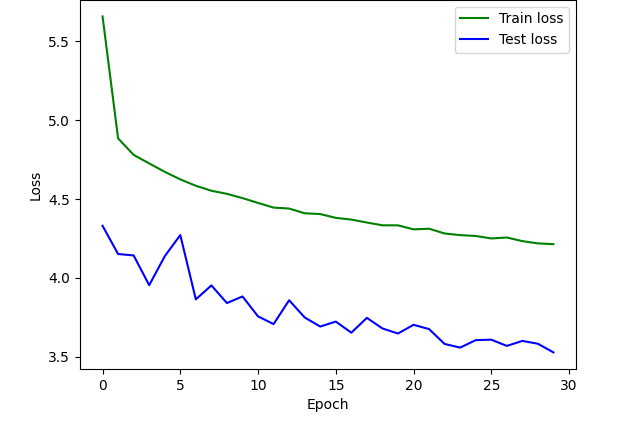
\includegraphics[width=\textwidth]{images/Experiments/training_size/train_test_losses_cropped.png}
        \caption{Train-Test losses of the selected "best candidate" transformer model on 30 epochs}
        \label{fig:train_best_30_epochs}
    \end{minipage}
    \hfill
    \begin{minipage}[t]{0.45\textwidth}
        \centering
        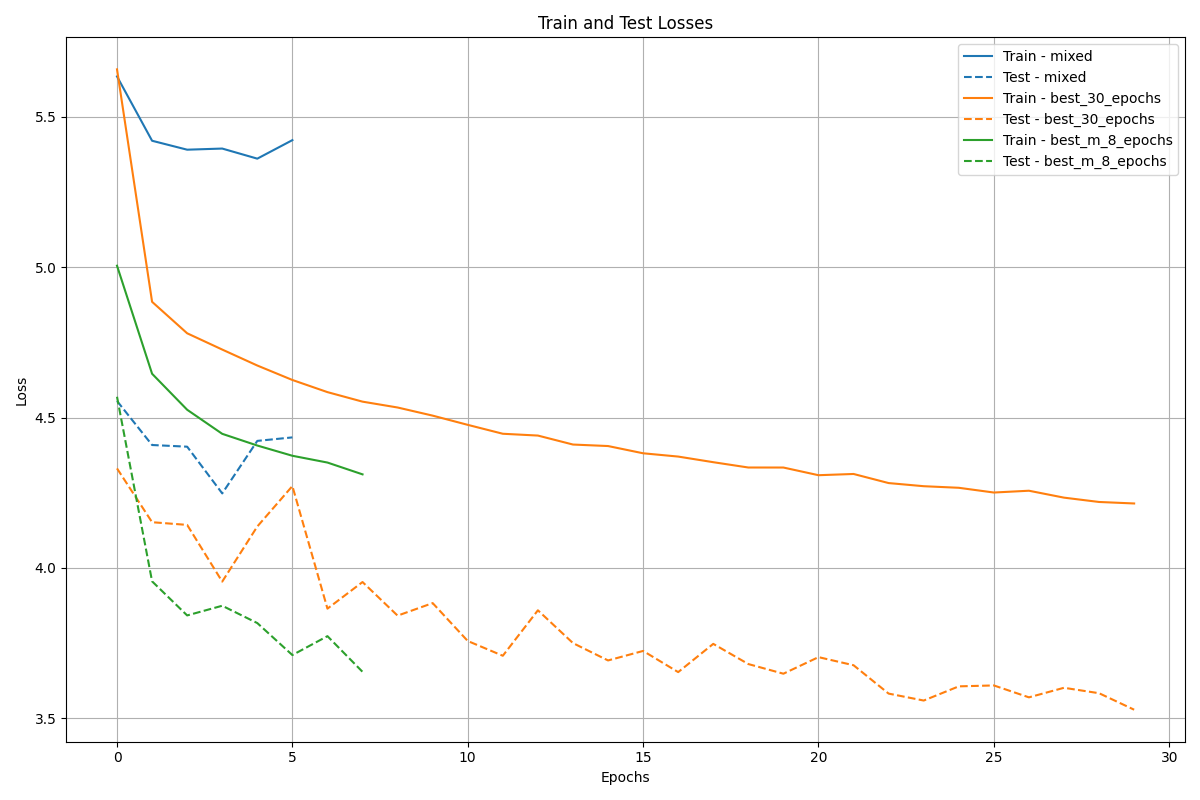
\includegraphics[width=\textwidth]{images/Experiments/training_size/train_test_losses_all_epochs.png}
        \caption{Comparison of the training results of the models on small and medium datasets}
        \label{fig:train_4_8_30_comaprison}
    \end{minipage}
    \label{fig:train_4_8_30_losses}
\end{figure}

The training on 30 epochs in the figure \ref{fig:train_best_30_epochs} shows no sign of plateau and a steady decrease of the training and testing losses.
Additionally, the cross-comparison in the figure \ref{fig:train_4_8_30_comaprison} shows that both the model training for 30 epochs on the small dataset and the model 
training for an equivalent of 8 epochs on a medium dataset show a steady learning curve. They both greatly outperform the model running on 4 epochs and
converge to a similar final training and test loss.

\begin{figure}[H]
    \centering
    
\includegraphics[scale=0.3]{images/Experiments/training_size/distances_list_all_models_all_signals.png}
    \caption{Comparison of the result in distances for the models on small and medium datasets}
    \label{fig:distance_signals_4_8_30}
\end{figure}

In terms of distances, both the small and medium dataset models outperform the model trained on 4 epochs as seen on the figure \ref{fig:distance_signals_4_8_30}.
The two long-training models yield very similar results on early stopping - meaning they have a very close distance to the signal considering a prediction limited 
to the original signal length-, with the model training on the small dataset having slightly better DTW distances meanwhile the medium dataset being slightly better 
on point-to-point distances.

\begin{figure}[H]
    \centering
    
\includegraphics[scale=0.3]{images/Experiments/training_size/diff_list_all_models_all_signals.png}
    \caption{Comparison of the result in image shapes for the models on small and medium datasets}
    \label{fig:diff_signals_4_8_30}
\end{figure}

Lastly, both longer training models once again outperform the baseline predictions. However, the 30 epochs model has a consistent better median than the 8 epochs model, 
hinting at shapes that are more sticky with regard to the original skeletons. \\ 

Training the model for longer has benefits: the losses have a consistent decrease over a larger longer of periods, and the resulting predictions are better in terms of distances and shapes. Additionally, there is little noticeable difference between training for a longer number of epochs or for a larger amount of data, although the validation dataset is randomly sampled and might thus not be diverse enough to test the generalization capabilities that training on different signals should bring.\par
The total number of passes of the data amounting to \(32M\) datapoints does not seem to reach the limit of the trainability of the models, and it might be possible to 
train further and obtain better results. This amount of data is reaching the levels that are recommended for transformers.

\section{LSTM Ablation study}
Finally, we proceed to an ablation study by having the best candidate over 30 epochs trained with and without an LSTM guiding unit in order to compare their performance.

\begin{figure}[H]
    \centering
    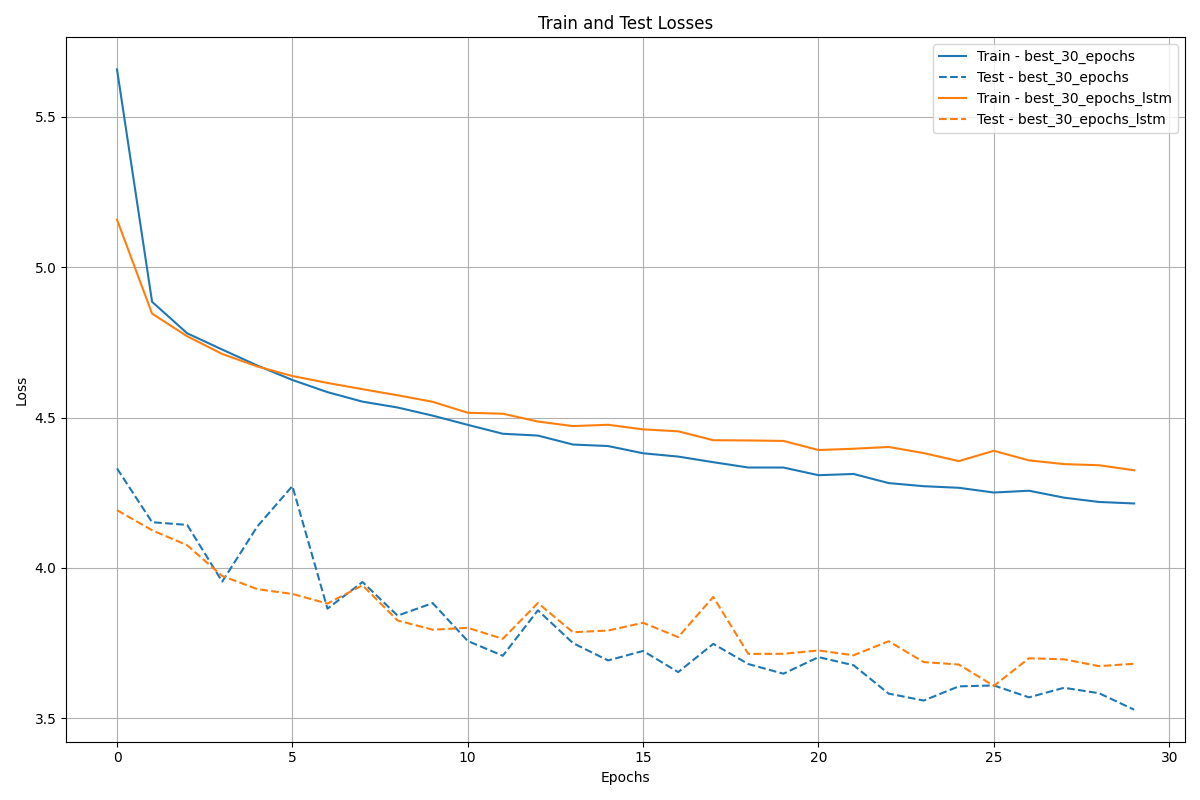
\includegraphics[scale=0.3]{images/Experiments/lstm_ablation/lstm_no_lstm.png}
    \caption{Comparison of the training of a model on 30 epochs with and without an LSTM unit}
    \label{fig:ablation_lstm_study}
\end{figure}

The performances of the model with and without the LSTM unit are plotted in the figure \ref{fig:ablation_lstm_study}. Some of the earlier observations
still stand as the LSTM model seems to be converging slightly faster with a noticeable difference over the first few epochs. Furthermore, the end results 
of the model have very little difference with the LSTM-guided model having a slightly lower convergence rate over the full epochs.\par
This observation is the same over the sequences length, distances and image differences as shown in the appendix \ref{section:appendix_lstm} on the figures
\ref{fig:a1}, \ref{fig:a2} and \ref{fig:a3}: neither of the model outperforms the other, meaning the LSTM unit has been mainly used very early in the training 
phase without impacting the latter stages.

\chapter {Conclusion and Future Work}
%In which we step back, have a critical look at the entire work, then conclude, and learn what lies beyond this thesis.
In this section, we summarize the results of the model and conclude on the strength, weaknesses, and future works of the present project.

\section{Results}
For this section, we use the predictions of the best candidate trained on 30 epochs on the small dataset to observe the quality of the signals produced and draw conclusions on its capacities.

\begin{figure}[H]
    \centering
    \begin{minipage}[t]{1\textwidth}
        \centering
        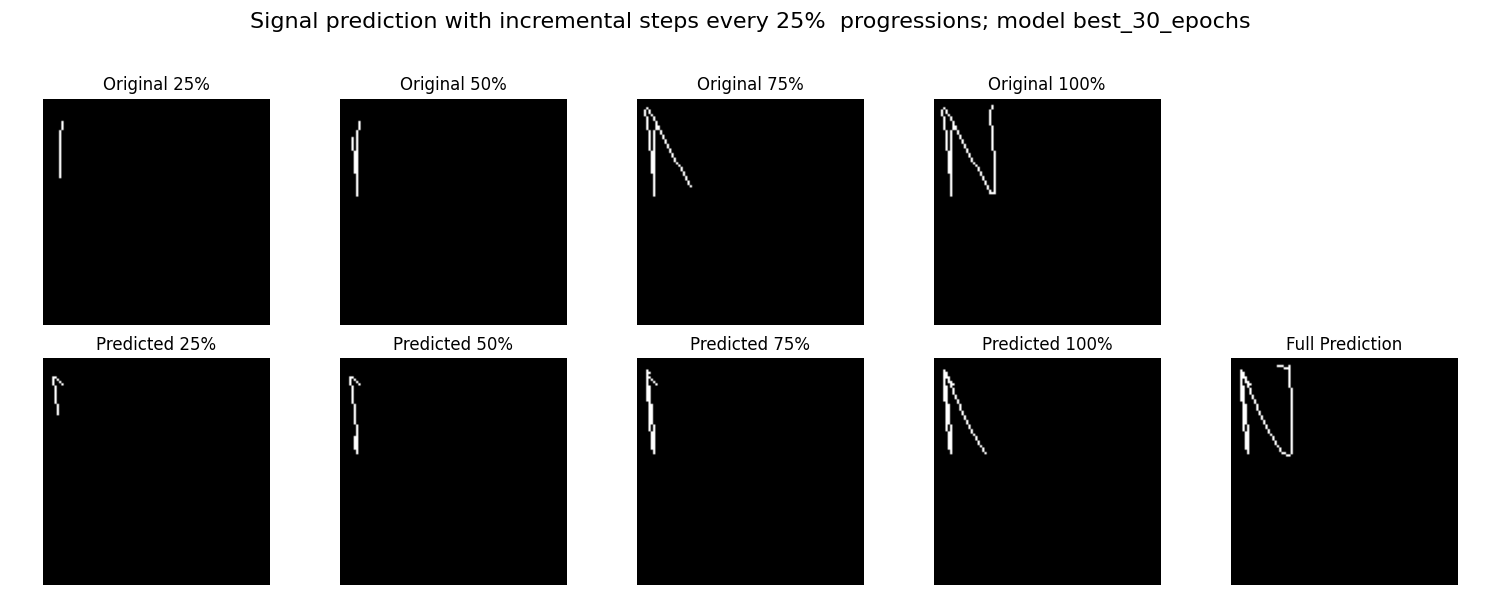
\includegraphics[scale=0.3]{images/Results/good_result_N.png}
    \end{minipage}
    \vspace{0.5cm} % Space between the two images
    \begin{minipage}[t]{1\textwidth}
        \centering
        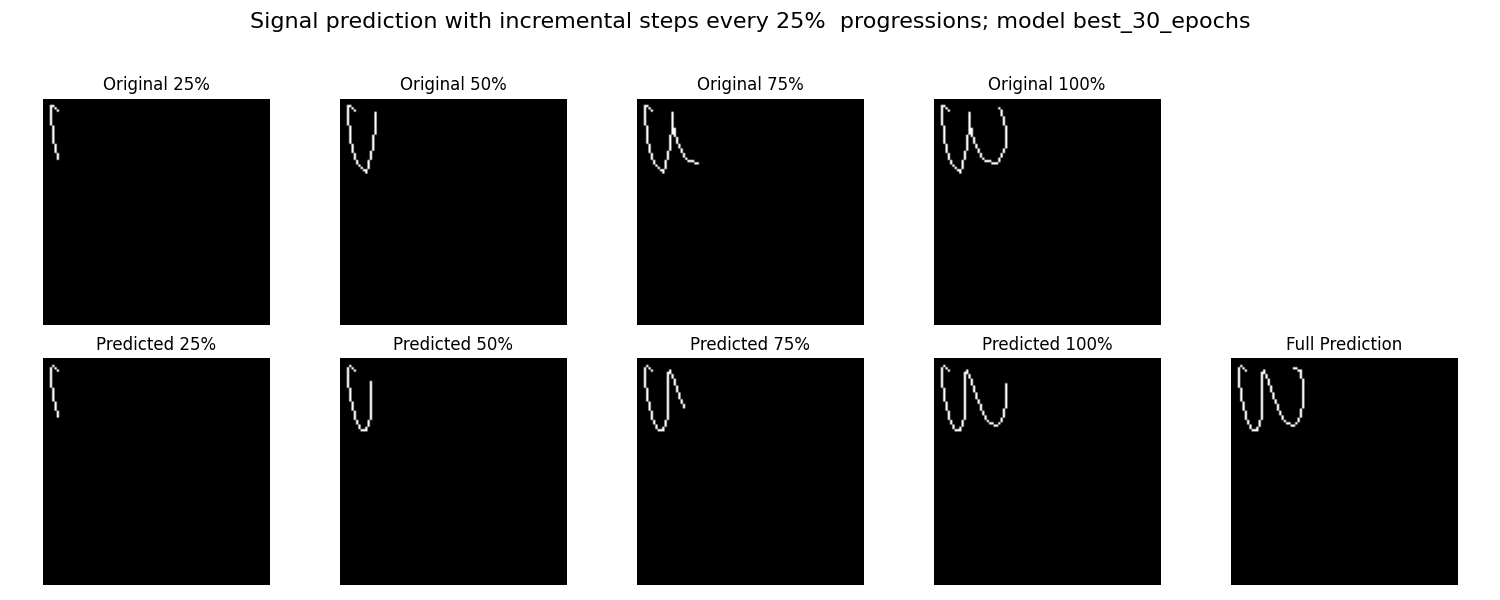
\includegraphics[scale=0.3]{images/Results/very_good_w.png}
    \end{minipage}
    \caption{Comparison of the original and predicted signals, good results on N and W.}
    \label{fig:good_results}
\end{figure}

On smalls signals, the model is able to perform very good prediction as shown in the figure \ref{fig:good_results}. On the top prediction, we can observe that the model
has learned a very good representation of the ductus of the English language for the letter "N", as it starts by going downward in the first vertical edge before going back 
in its track to finish the shape, albeit at a slower pace compared to the original writer. In the bottom prediction, the model writes an almost perfect 
cursive "w", with a very good speed relative to the original writer at each time step.\par
To give some perspective over the metrics used for comparison during the experiments, the above prediction scored \([52\%,48\%,50\%]\) on image matching and \([97, 149]\) on DTW and Point-to-Point Euclidean distance while the below prediction scored \([44\%,40\%,42\%]\) matching and \([167, 435]\) DTW and distance. These results are located between the average and the third quartile 
for the model, meaning they are good scorer but not outliers, whereas they could be considered as very good predictions.

\begin{figure}[H]
    \centering
    \begin{minipage}[t]{1\textwidth}
        \centering
        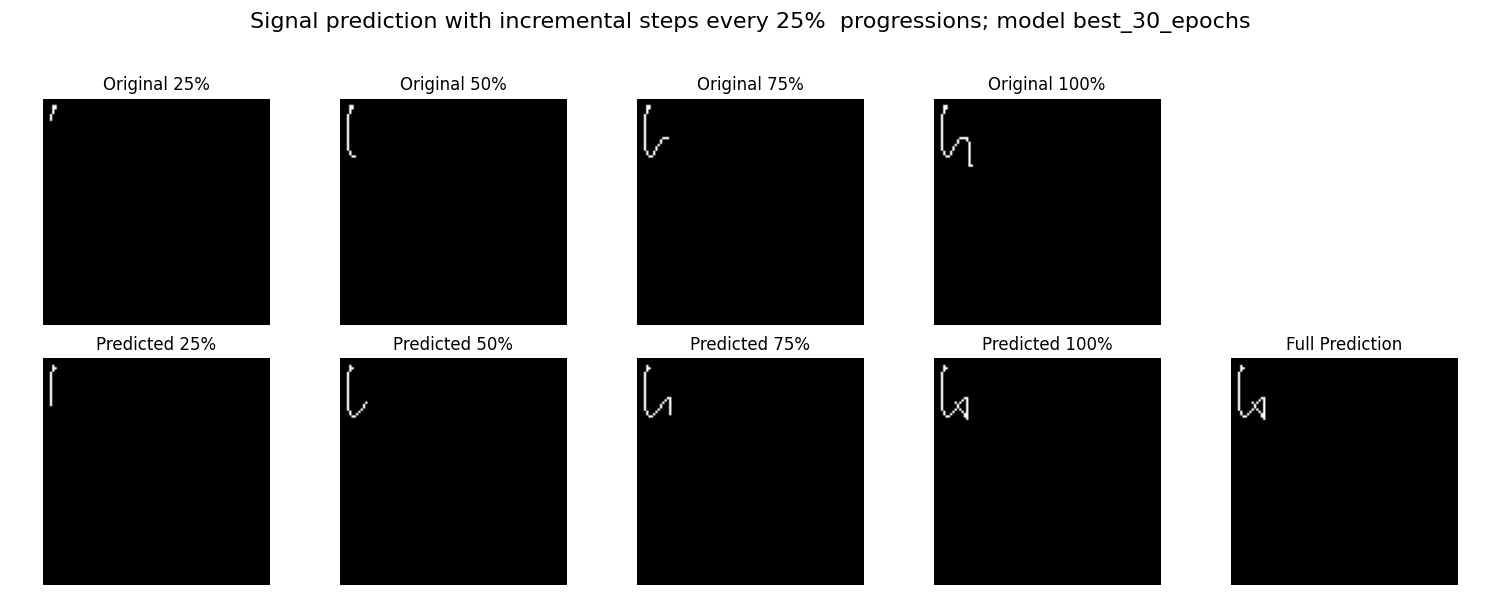
\includegraphics[scale=0.3]{images/Results/not_stopped_h.png}
    \end{minipage}
    \vspace{0.5cm}
    \begin{minipage}[t]{1\textwidth}
        \centering
        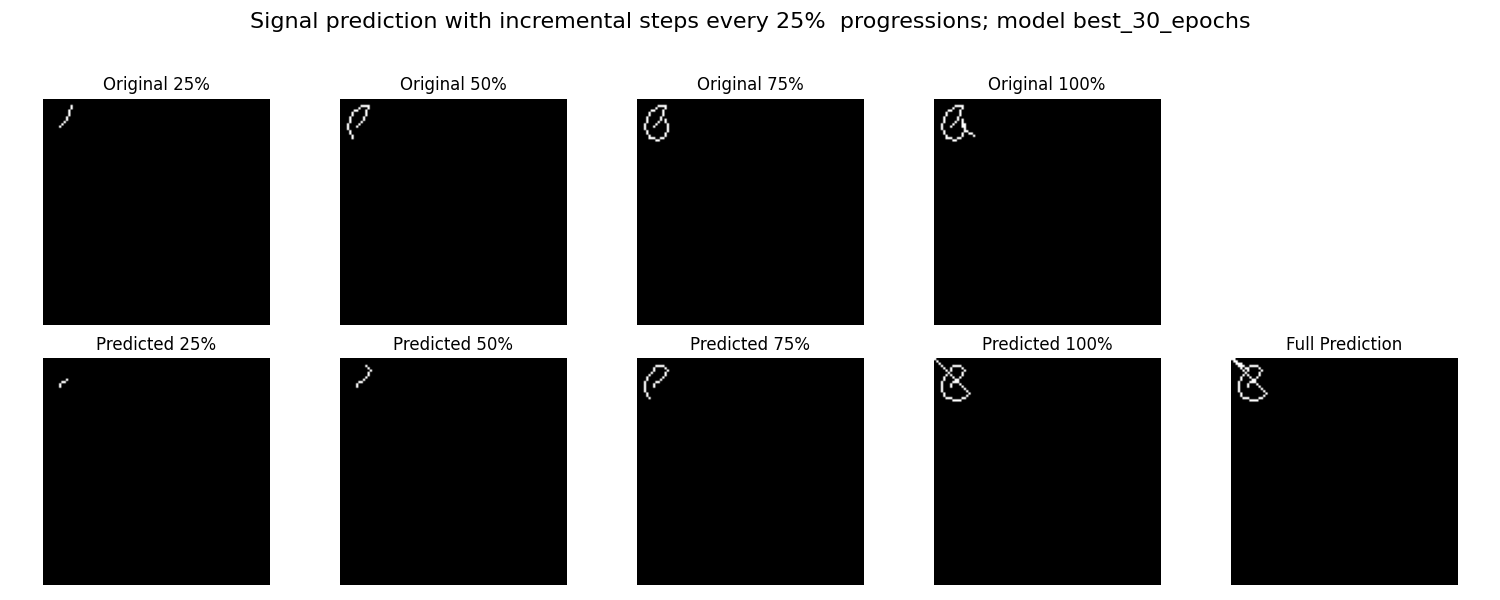
\includegraphics[scale=0.3]{images/Results/failure_to_stop.png}
    \end{minipage}
    \caption{Predictions with a failure to stop at the end of the generation}
    \label{fig:failure_to_stop}
\end{figure}

One of the sources of errors from the model comes from its failure to stop the prediction once it cannot generate further coordinates. The situation is greatly 
improved on models that train for a long time whereas the models trained on 4 epochs never predict an EOS token at all.\par
However, the figure \ref{fig:failure_to_stop} shows that even the long-training model still have lingering curves, 
even on very good predictions. The example on top shows a cursive "h" with the model still predicting a little line before stopping the prediction, adding the EOS slightly too late. The bottom example shows the same behavior with a slightly more extreme leftover line. This great line going to the source is a 
sign that the model tries to predict an EOS token located at the coordinates \([-1; -1]\) but doesn't quite reach it. In failing to do so and because the EOS 
token is very sensitive and reacts only to these exact coordinates, predicting any close location such as \([-0.5; -0.5]\) results in a line being drawn towards the source.
Often times, the model predicts this close coordinate to the EOS token followed by the EOS token, with this single prediction having a high impact on the results.\par
This badly influences every metric as the line adds a lot of wrong pixels for the skeleton loss during training and for the distances and image differences during evaluation 
whereas the predicted signal is overall very good.\par
This could be solved via heuristic solutions by manually checking the very last coordinates of the predicted signals and eliminating obvious near-EOS failures or by being more lenient on 
the definition of the EOS token (for example, by considering every negative coordinate as meaning EOS).
Another solution has been proposed and tested with some outputs with the notion of ink. In addition to letting the model stop the signal itself, the total distance
traveled by the pen can be considered as the ink used to write the signal. By limiting the ink of the generated signal to the ink of the original signal, such overdrawing 
can be limited.

\begin{figure}[H]
    \centering
    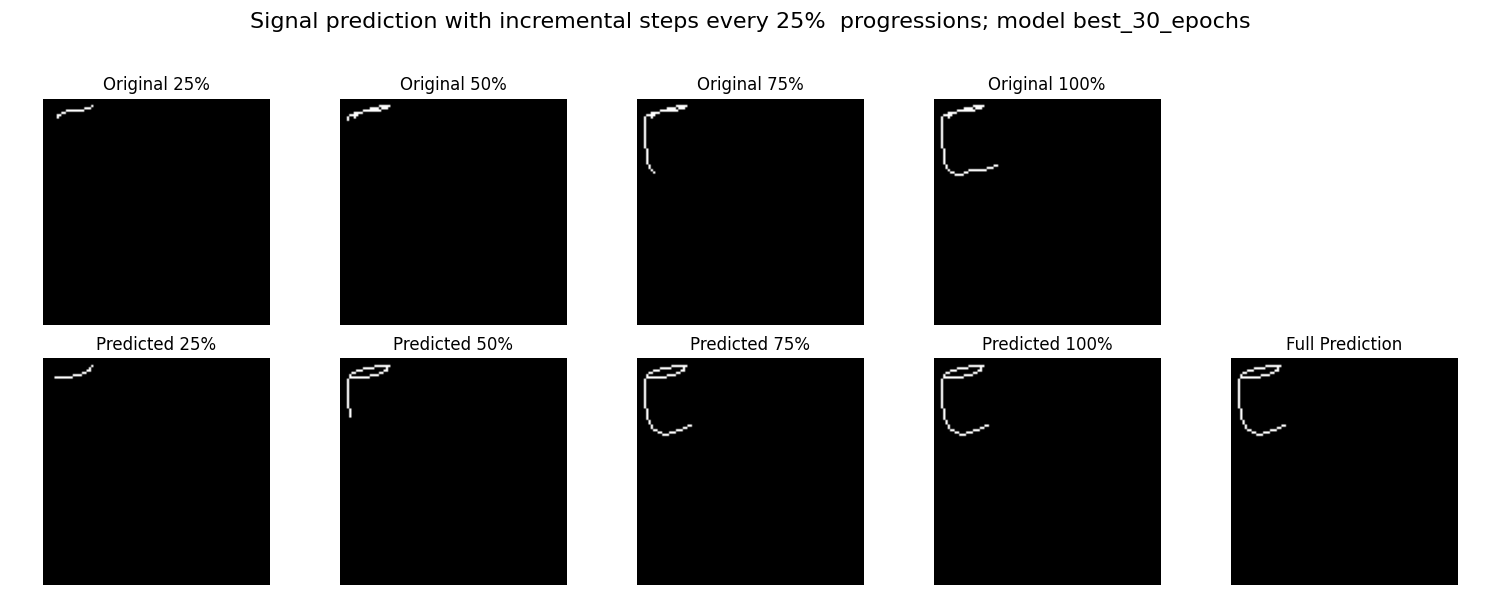
\includegraphics[scale=0.3]{images/Results/trying_to_write_e.png}
    \caption{Prediction with a recognition error leading to small noticeable changes}
    \label{fig:other_failures}
\end{figure}

The model has other sources of errors on the small signals. The figure \ref{fig:other_failures} shows a very interesting example of failure, although this 
does not represent an exhaustive list of all possible causes of bad predictions.\par
The original image represents an open square bracket whereas the model instinctively recognized it as the letter "e" and has therefore predicted 
this variation while still respecting the overall shape of the image. This can be due to an insufficient amount of examples of the square brackets in the training data: if the model has no example 
of ductus of a character, it is very hard to "invent" a way of writing it, and it might prefer to write a known letter. This means that the model 
has learned an alphabet of symbols that it is able to write and would probably have difficulty in doing zero-shot predictions. \\ 

\begin{figure}[H]
    \centering
    \begin{minipage}[t]{1\textwidth}
        \centering
        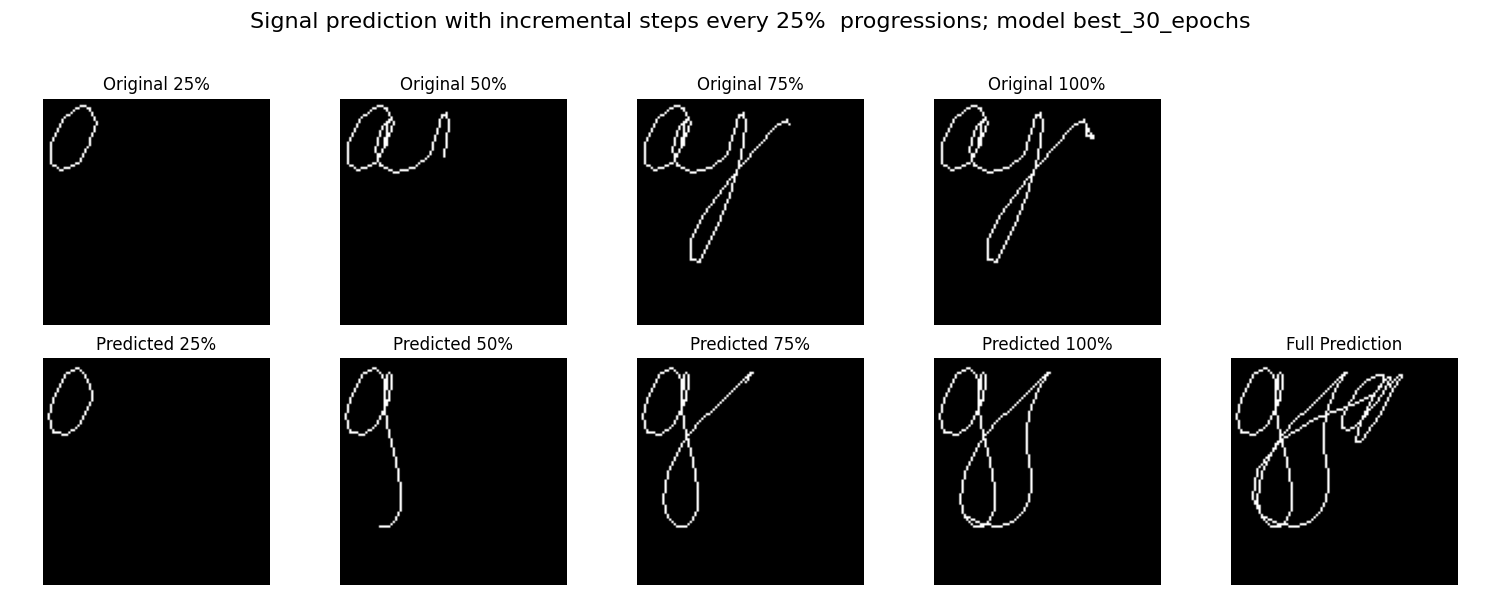
\includegraphics[scale=0.3]{images/Results/large/mistook_letter.png}
    \end{minipage}
    \vspace{0.5cm}
    \begin{minipage}[t]{1\textwidth}
        \centering
        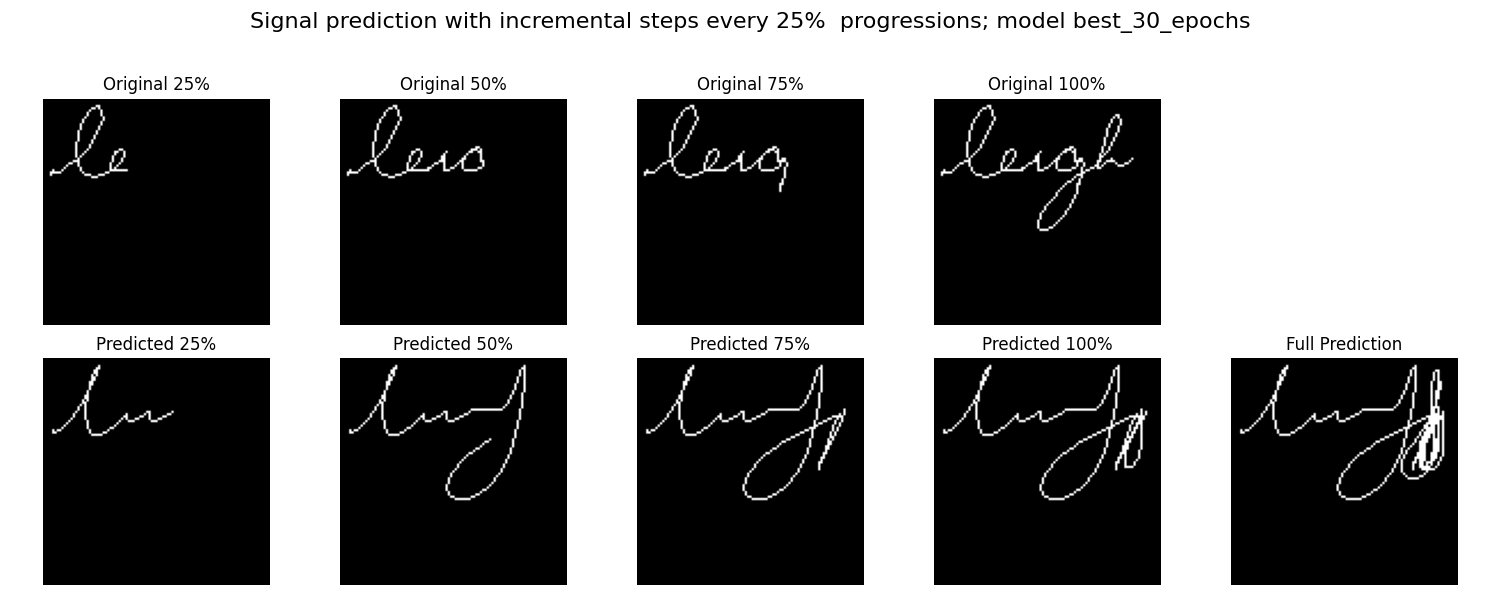
\includegraphics[scale=0.3]{images/Results/large/sketchy.png}
    \end{minipage}
    \caption{Predictions with a failure to stop at the end of the generation}
    \label{fig:failures_large_signals}
\end{figure}

Large signals are way harder to correctly predict for the model which is generally better at recognizing and copying individual characters. 
The two examples on the figure \ref{fig:failures_large_signals} show a tendency to generate sketches that have a correlation in the shapes of the 
characters, but do not stick correctly to the overall skeleton. The writings share some features, such as big curves for "L"s and "G"s, but the 
predictions are not legible without the original signals. The bounding boxes are well respected, which indicates that the model still paid attention 
to the overall signal, but the result is essentially a sketch or scribble looking like the original and less precise than individual characters.\par
The example on top shows the model generating a "g", attaching the first "a" to the bottom loop, and attaching another "j" to that same loop. Large 
signals go beyond the context limit that was set to 100 coordinates, and the loss of context could be a source of this loss of precision on large signals.

\begin{figure}[H]
    \centering
    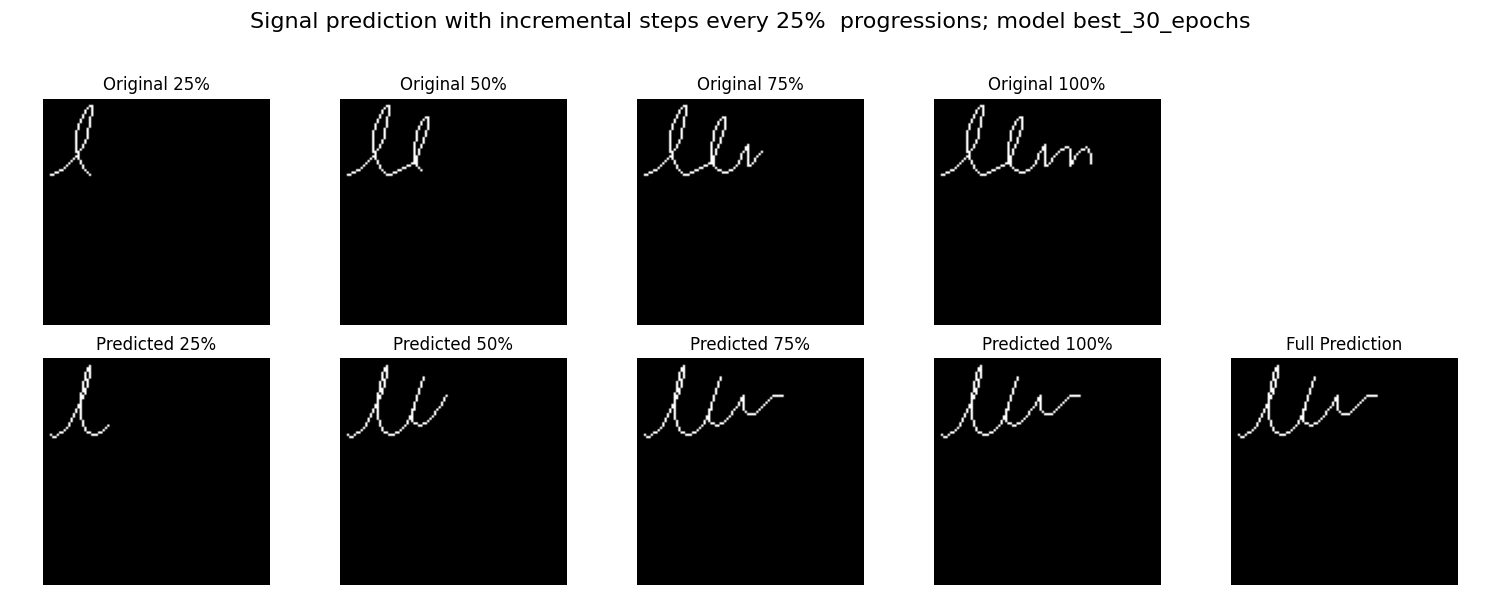
\includegraphics[scale=0.3]{images/Results/large/llm_almost.png}
    \caption{Prediction of the "LLM" word by the model}
    \label{fig:llm}
\end{figure}

Finally, we show that the model can almost write its cousin's title properly, 
paying homage to the Large Language Models that inspired its architecture, as seen in the Figure \ref{fig:llm}.\\

Our model is able to predict very precise coordinate signals on what's defined as "small signals" under 50 coordinates to predict, with very convincing shapes and speeds. It appears that it does so by learning an alphabet of characters form which the general ductus are learned. Multiple examples show that the model adapt the basis ductuses to the variations in shapes by the writer, and the generated signal show good respect for the location and bounding boxes of the images. One remaining issue on large signals is the EOS generation: making models learn for longer allowed them to learn to generate EOS to an extent, but we still observe some failures to do so. \par
The generation on large signals is more complex and the results are less convincing. The predictions are often scribbles with general shapes (big curves, loops, bounding boxes) respecting the original signal, but the predictions are hardly legible. The model is still able to react to very large letter and words, and seems capable of generating the start of the signal until the point where it gets lost and stops. Although the limitation to large signals is currently a large handicap to bear, we could imagine a mechanism of pre-division of the large signals into smaller sub-signals to ingest. To describe a full sentence from an offline image, the SET, SORT! transformer can be used to obtain the set of ordered sub-strokes composing the overall writing, and have each substroke processed by our model, resulting in the full 
coordinate vector of the image.
\par
The model seems able to generalize on individual learned characters but is not able to predict zero-shot samples: if a character is unseen, it will probably not 
be predicted correctly. This means that the training of the model must be adapted to the task it has to solve, and obtaining a model to work with the papyrus will require 
to find an adapted annotated dataset large enough to train on.\par

\section {Future works}
During the implementation of the project, multiple axes of explorations have been identified. 
This section lists propositions of future works that can enhance the results obtained in this report. \\

The model uses absolute coordinates in its training data and predictions. The skeleton losses and image differences are metrics that are focused on point-to-point, pixel-wise 
match of the shapes. This means that an almost-perfect shape that has a constant offset of 1px in either direction would be considered bad in terms of 
shape meanwhile it should be regarded as a good prediction.\par
By changing the coordinates from absolute to relative, the prediction could be more agnostic to these offsets. Instead of predicting a vector of \([x,y]\) coordinates,
each element of the signals can be switched to relative movement from one another. Each target token would be a speed vector over the frequency, and the signal 
would be re-constructed by following the path point-by-point. With this method, a curve exactly reproduced with an offset would have the exact same representation 
in the vector. This requires work on the context management as this method requires at least one absolute coordinate per sequence to locate the vector in the image, and the representation of the EOS 
token could not be the same as \([-1;-1]\) is an acceptable value in this domain. \\

With more hardware available, we recommend to search again for the best configuration on a wider set of hyperparameters. Additionally, 
we would have liked to use the BRUSH and UNIPEN datasets to their full extent. Adding more data will require more time to train but could offer a better model.\par
Additionally, the training data generated from the dataset can be upgraded. For example, by obtaining a better cut of the signals that respect the overall 
inertia and previous context of the signal, or by doing a stratification when extracting the train, test, validation datasets in order to have a balance 
of writers for BRUSH and providers for UNIPEN and overall characters between them. The question of whether all data is good to keep is also worth to be investigated.\\ 

The metrics used for the evaluation - matching images, DTW and distances - allow a comparison of the shapes of the generated signals, but are very sensible 
to offsets in the image. It is hard to find good evaluators and more exploration around this problematic would be helpful. For example, the image differences currently do a pixel count of the non-matching pixels meanwhile assigning further value to the pixels dependend on their distances to the skeleton, similarly as is done on the skeleton loss, would give a fairer and less binary evaluation of the shapes where being closer to the skeleton would be awarded.\\

The EOS signal issue and the overall low capacity of the models to stop the prediction, although alleviated when trained for a sufficient amount of time,
is still an issue to keep on the radar for enhancements. Some heuristic evaluations are currently in place to alleviate the issue, such as the ink stopping or the repeating coordinates detection, but the model should ideally call for the end of the signals itself.  \\ 

Lastly, in order to adapt this work for the papyrus collection's analysis, the question of transferable knowledge to other ductus could be interesting. There is 
very little online data to train on: online image is impossible to retrieve from original collections and can only be re-created as closely as possible with 
similar materials and supports. However, it will be a tedious task to recreate a dataset with the required amount of data, especially considering the hungriness 
of transformers that has been verified in the Experiments.\par
Very large vision and language models are usually pre-trained on large datasets aggregated from multiple sources and fine-tuned on smaller 
specific datasets for a given task. However, we observed some difficulty in out-of-distribution predictions and we do not know if 
the knowledge transfer can be done with a pre-training on a ductus and a fine-tuning on another (for example, from English to Greek).

\section{Conclusion}
In this work, we have introduced an architecture based on a combination of transformer-based models that is able to perform the challenging task of generating online signals from 
offline images. It generates very good predictions for small signals and respect overall shapes for large signals. The tentative of adding an LLM guiding unit to the model 
yields mitigated results as the predictions are almost identical.\\

We have identified a configuration that is able to produce good predictions on the limited system that was available for this thesis. We suggest that 
this architecture has not reached its ceiling and larger models with more layers, heads, and larger datasets could achieve even better results at the cost 
of more computational power. We have used \(5\ to\ 20\%\) of our smaller dataset, and we are excited to see the results of a model that would have access to the entire datasets,with the alignment work already integrated with our data pre-processing pipeline.\\

This work is not ready to be applied to for historical document analysis, but can hopefully help pave the way for future study that can test the model architecture on further tasks such as dating, authorship determination or synthetic images creation. We are particularly curious
about the adaptability of the model in generalizing its understanding to other characters, ductus, and general domain of application for the very specific world of Greek Papyrus. \\ 

The results are promising and respond to the question of this proof-of-concept: A transformer model is capable of predicting the pen kinematics from 
offline images \textit{on the English language, with a sufficient dataset and on a restricted alphabet of symbols}.\\

\appendix
\chapter{Appendix}

\section{Training Experiment Additional Results} \label{section_appendix_train}

\begin{table}[h!]
    \centering
    \begin{tabular}{|l|p{7cm}|p{7cm}|}
        \hline
        \textbf{Model} & \textbf{Train Loss (per epoch)} & \textbf{Test Loss (per epoch)} \\ \hline
        Mixed & 
        \texttt{[5.6347, 5.4208, 5.3910, 5.3948, 5.3612, 5.4228]} & 
        \texttt{[4.5552, 4.4087, 4.4032, 4.2478, 4.4224, 4.4341]} \\ \hline
        Best 30 Epochs & 
        \texttt{[5.6583, 4.8850, 4.7804, 4.7262, 4.6731, 4.6251, 4.5847, 4.5530, 4.5335, 4.5065, 4.4758, 4.4462, 4.4402, 4.4103, 4.4053, 4.3812, 4.3703, 4.3516, 4.3339, 4.3338, 4.3083, 4.3124, 4.2821, 4.2717, 4.2665, 4.2507, 4.2567, 4.2337, 4.2193, 4.2143]} & 
        \texttt{[4.3309, 4.1519, 4.1430, 3.9544, 4.1377, 4.2722, 3.8645, 3.9530, 3.8412, 3.8829, 3.7568, 3.7077, 3.8590, 3.7499, 3.6921, 3.7238, 3.6533, 3.7473, 3.6801, 3.6480, 3.7032, 3.6762, 3.5819, 3.5588, 3.6060, 3.6090, 3.5694, 3.6012, 3.5831, 3.5283]} \\ \hline
        Best M-8 Epochs & 
        \texttt{[5.0051, 4.6457, 4.5260, 4.4459, 4.4070, 4.3730, 4.3504, 4.3111]} & 
        \texttt{[4.5692, 3.9553, 3.8419, 3.8741, 3.8165, 3.7101, 3.7730, 3.6543]} \\ \hline
        \end{tabular}
        \caption{Train and Test Losses per epoch for Mixed, Best 30 Epochs, and Best M-8 Epochs Models}
    \label{tab:losses}
\end{table}

\section{LSTM Additional results} \label{section:appendix_lstm}

\begin{figure}[h!]
    \centering
    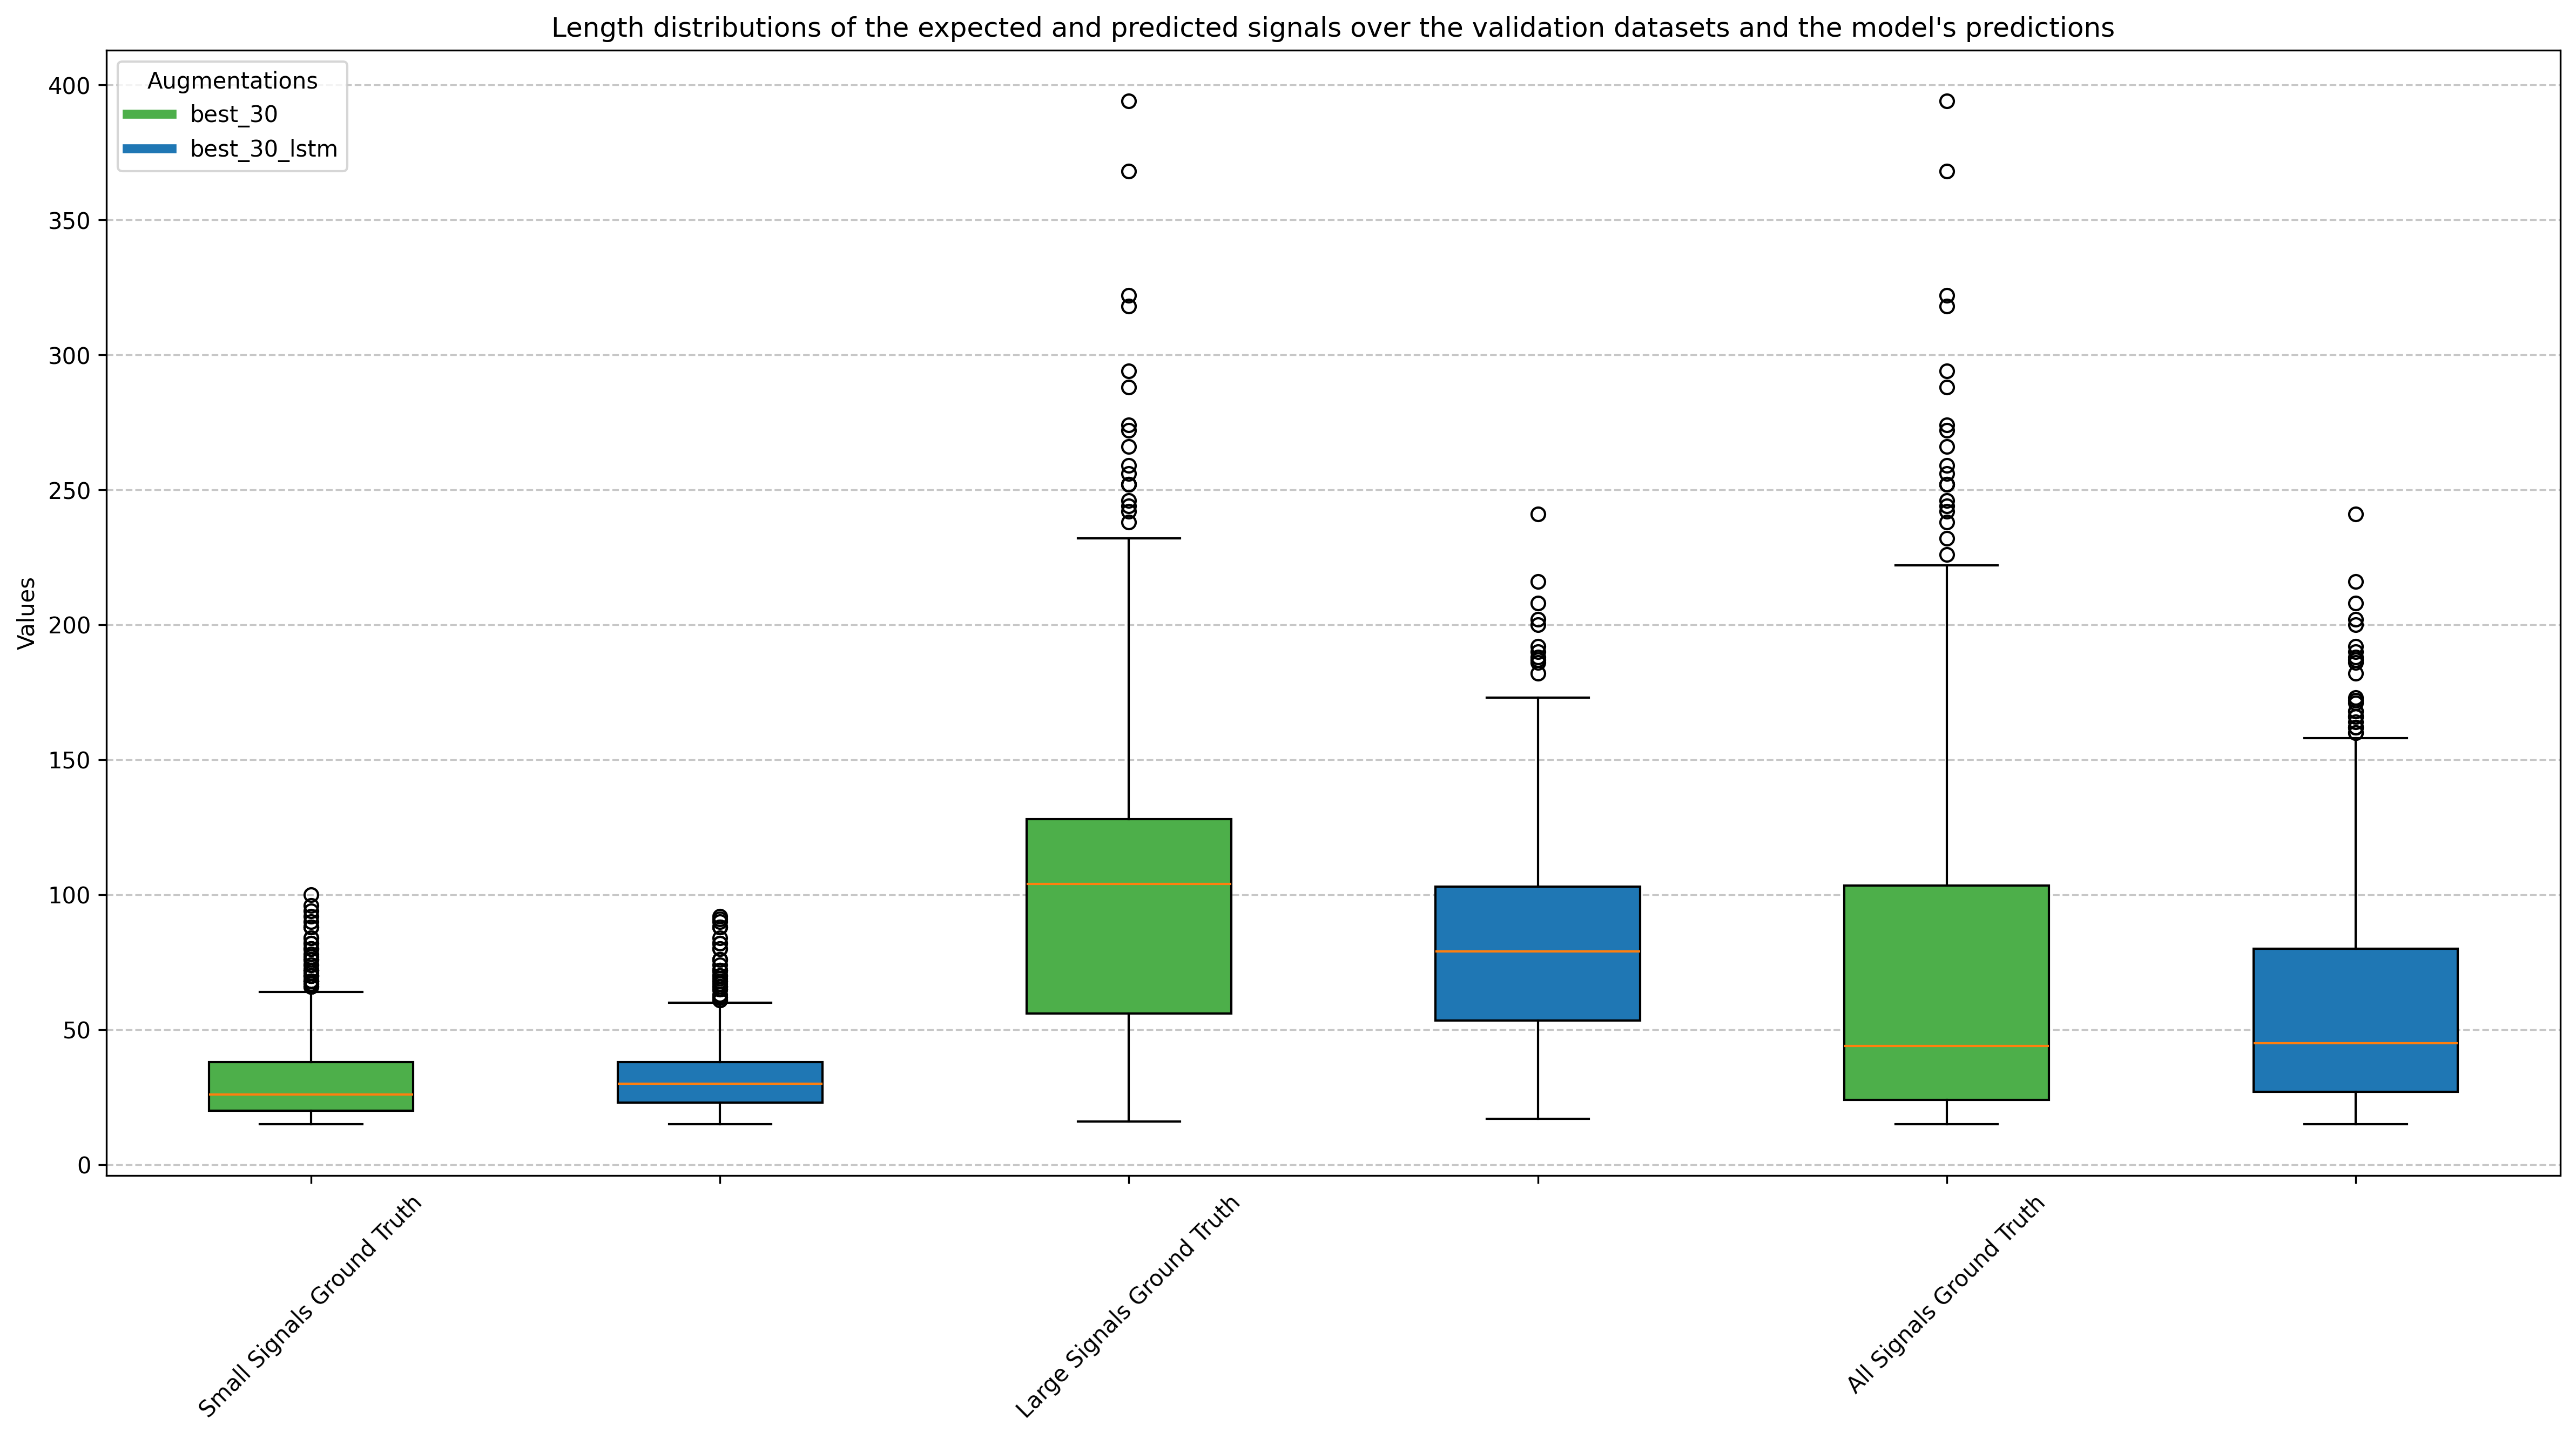
\includegraphics[scale=0.3]{images/Experiments/lstm_ablation/length_distribution.png}
    \caption{Length distribution comparison of a model trained on 30 epochs with and without a guiding LSTM}
    \label{fig:a1}
\end{figure}

\begin{figure}[h!]
    \centering
    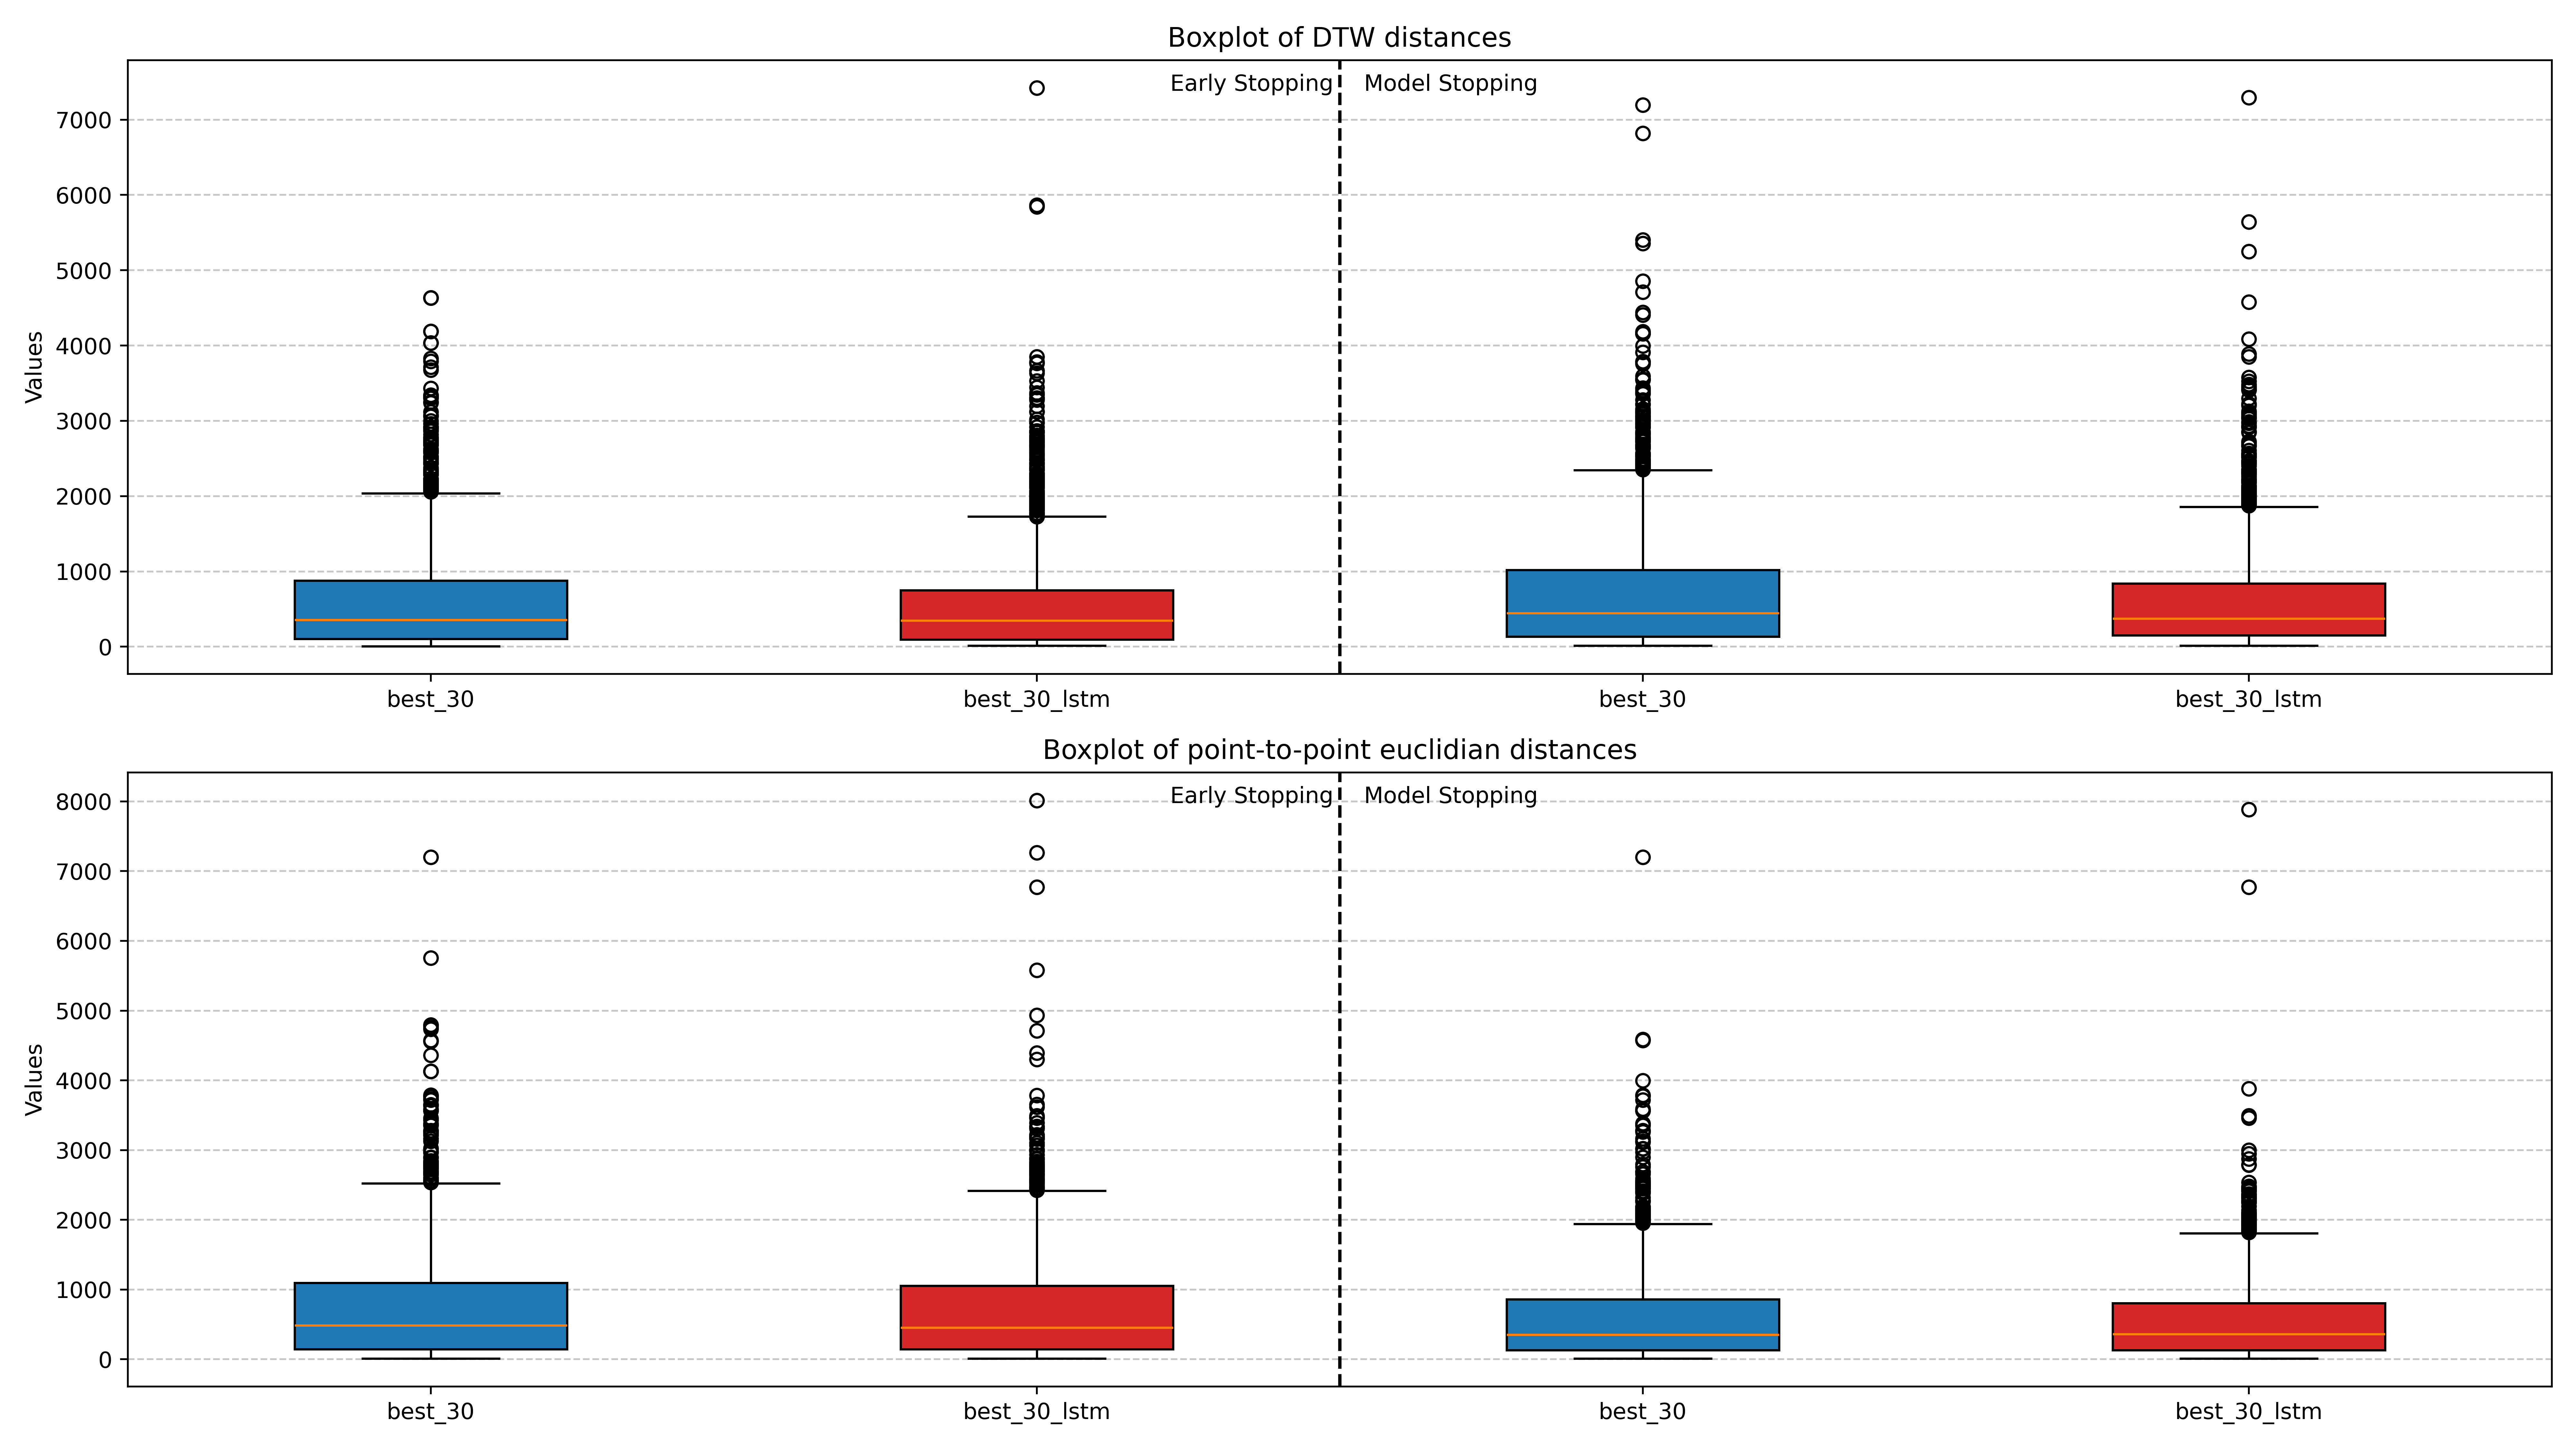
\includegraphics[scale=0.3]{images/Experiments/lstm_ablation/distances_list_all_models_all_signals.png}
    \caption{Predicted signals distance comparison of a model trained on 30 epochs with and without a guiding LSTM}
    \label{fig:a2}
\end{figure}

\begin{figure}[h!]
    \centering
    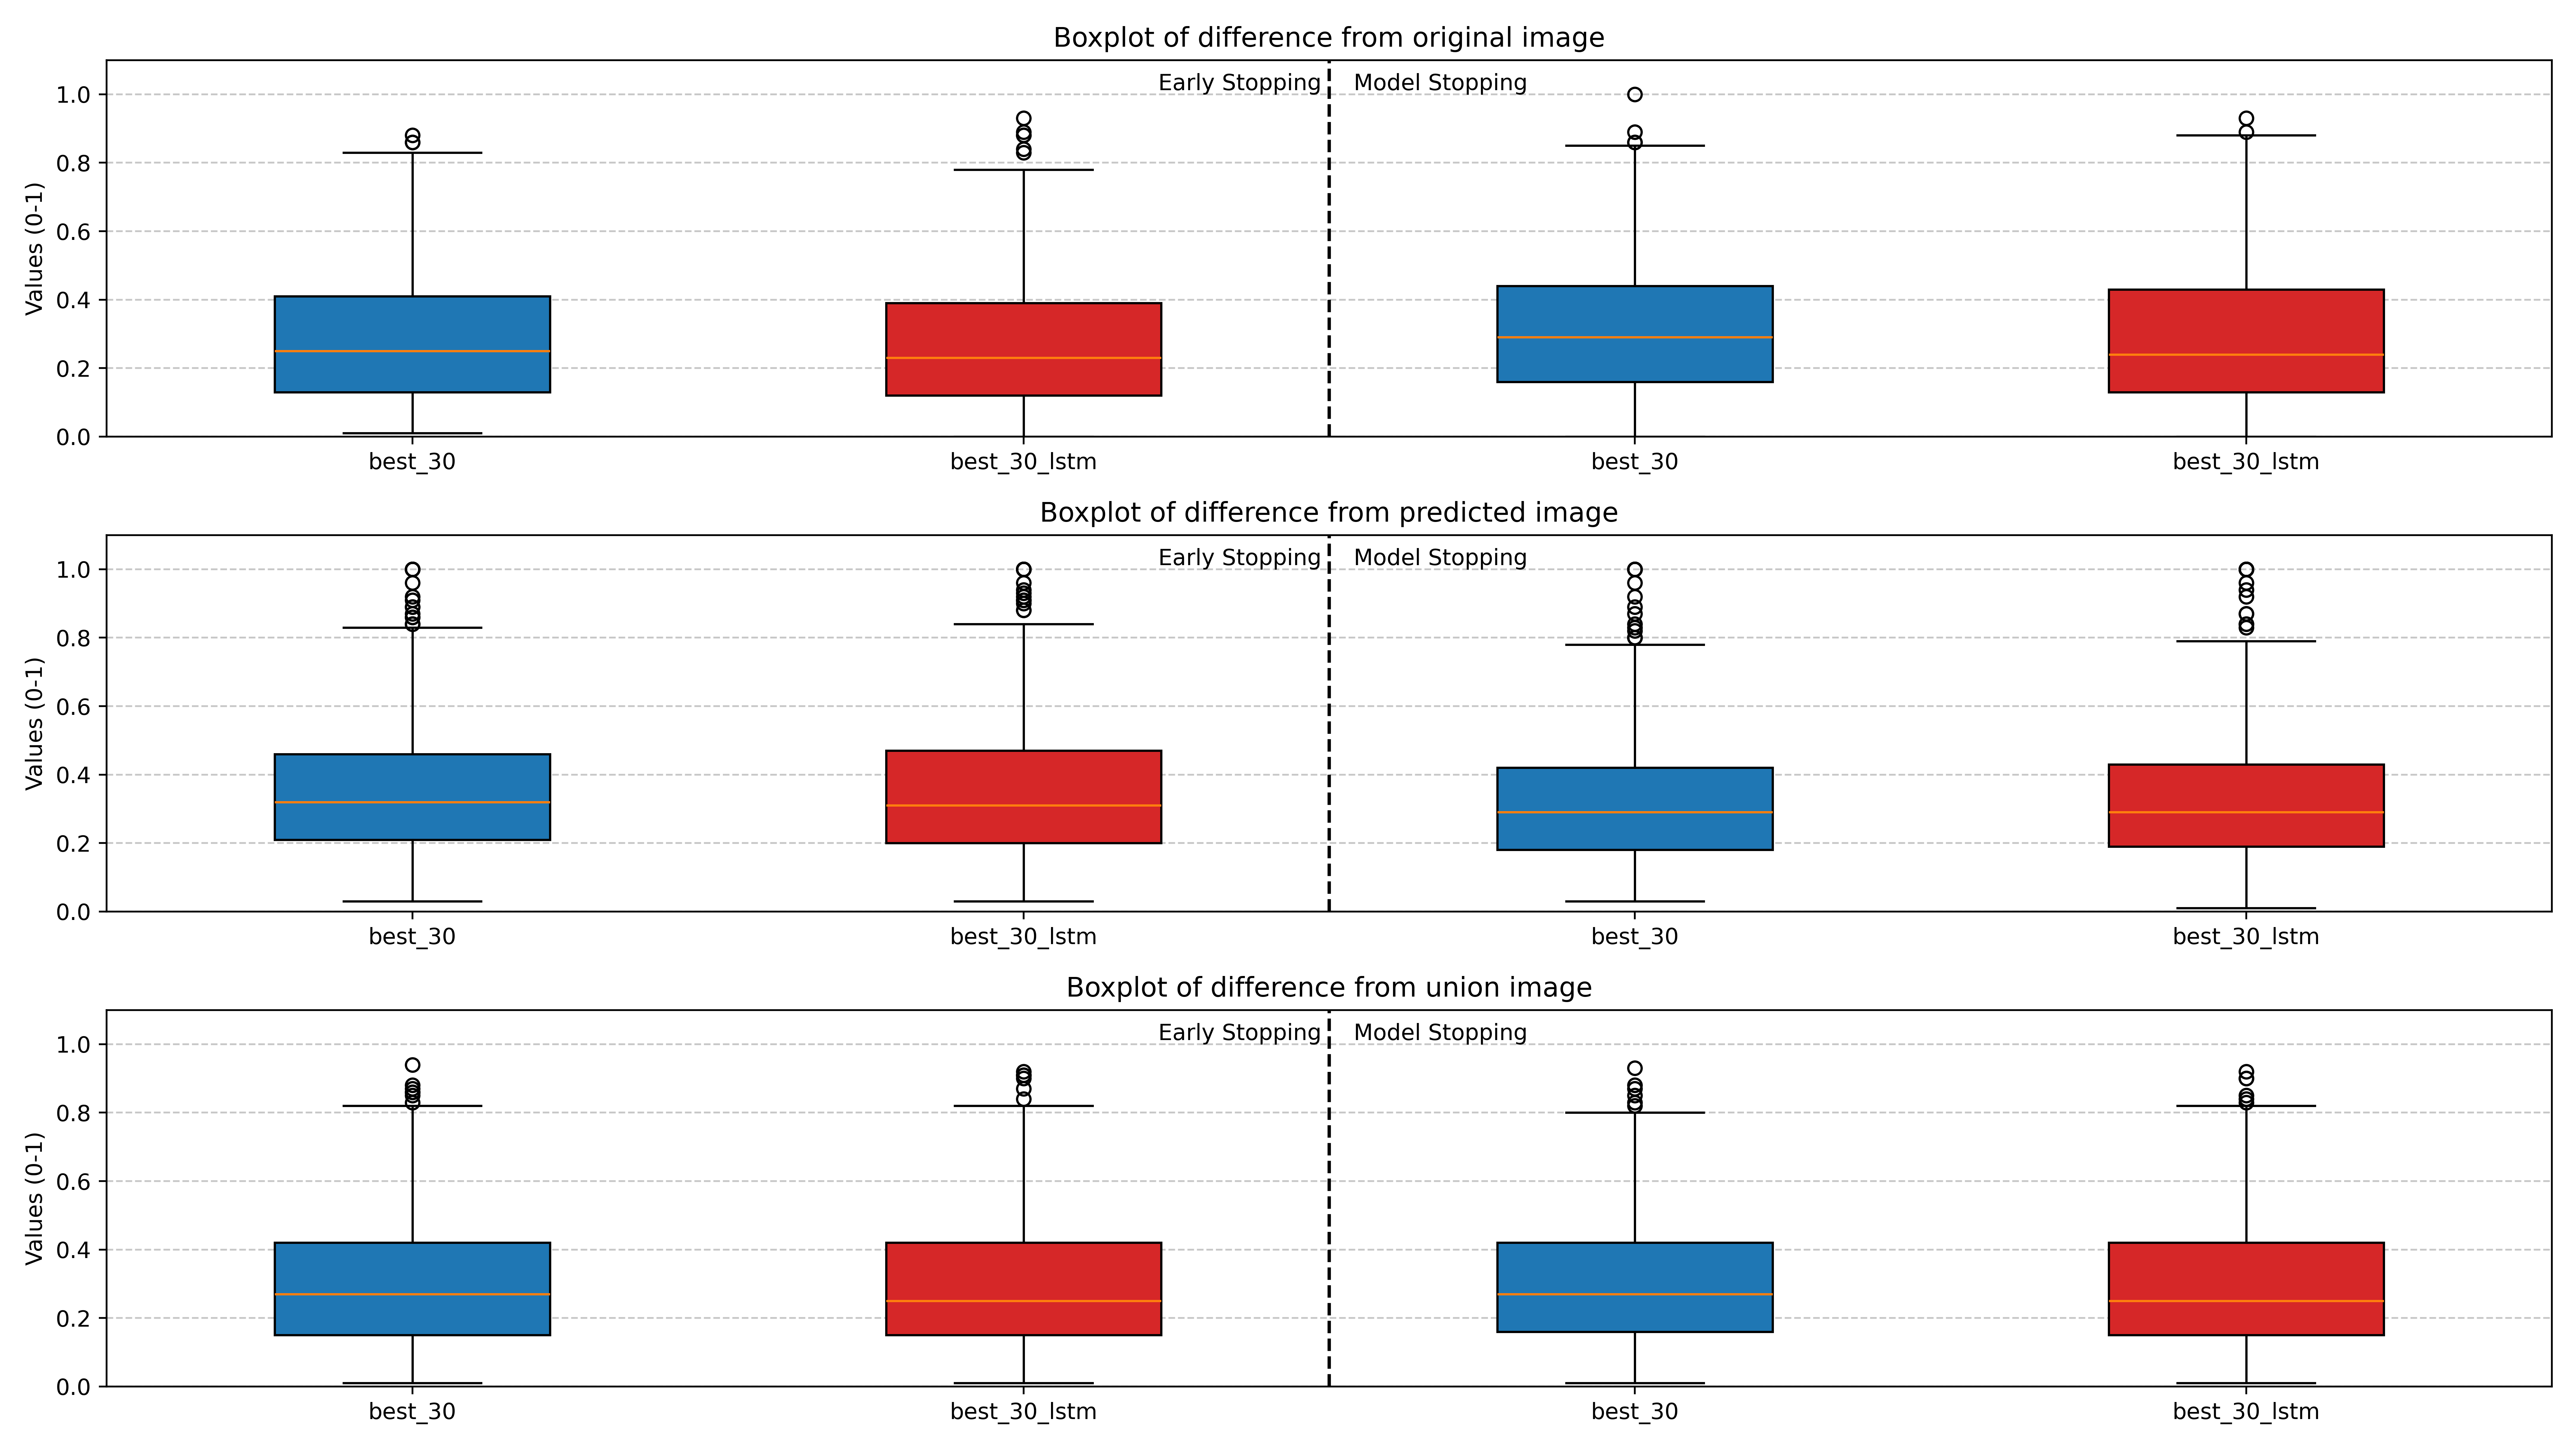
\includegraphics[scale=0.3]{images/Experiments/lstm_ablation/diff_list_all_models_all_signals.png}
    \caption{Predicted signals image difference comparison of a model trained on 30 epochs with and without a guiding LSTM}
    \label{fig:a3}
\end{figure}

%END Doc
%-------------------------------------------------------

\bibliography{bibliography}
\bibliographystyle{plain}

\end{document}